%\documentclass[twoside]{pwrthesis}
\documentclass[twoside]{iisthesis}
% ---

\usepackage{polski}
\usepackage[utf8]{inputenc}
\usepackage{amsmath}
\usepackage{tocloft}
\usepackage{listings}
\usepackage{algorithm}
\usepackage{algorithmic}
\usepackage{subcaption}
\usepackage{mathtools}
\usepackage{graphicx}
\usepackage[colorinlistoftodos,prependcaption,textsize=tiny]{todonotes}
\usepackage{url}
\usepackage{pgfplots, pgfplotstable}
\pgfplotsset{compat=1.13}
\usepackage{array,tabularx}
\selectlanguage{polish}
% Dodane przeze mnie d
\usepackage{fancyvrb} % dla srodowiska Verbatim
\usepackage{color}
\usepackage{lscape}
\usepackage{longtable}
\usepackage[shortcuts]{extdash}

\let\lll\undefined
\usepackage{amssymb}

\hypersetup{
    colorlinks,
    linkcolor={black!50!black},
    citecolor={black!50!black},
    urlcolor={black!80!black}
}

\definecolor{gray}{rgb}{0.4,0.4,0.4}
\definecolor{darkblue}{rgb}{0.0,0.0,0.6}
\definecolor{cyan}{rgb}{0.0,0.6,0.6}

\lstset{
  basicstyle=\ttfamily,
  columns=fullflexible,
  showstringspaces=false,
  commentstyle=\color{gray}\upshape
}

\lstdefinelanguage{XML}
{
  morestring=[b]",
  morestring=[s]{>}{<},
  morecomment=[s]{<?}{?>},
  stringstyle=\color{black},
  identifierstyle=\color{darkblue},
  keywordstyle=\color{cyan},
  morekeywords={xmlns,version,type}% list your attributes here
}

\lstset{
  language=XML,
   literate={ć}{{\'c}}1
}
\renewcommand*{\lstlistingname}{Kod źródłowy}
% definicje kolorow
\definecolor{ciemnoSzary}{rgb}{0.15,0.15,0.15}
\definecolor{szary}{rgb}{0.5,0.5,0.5}
\definecolor{jasnoSzary}{rgb}{0.2,0.2,0.2}

% Konfiguracja verbatima
\fvset{
	frame=single,
	numbers=left,
	fontsize=\footnotesize,
	numbersep=12pt,
%	framerule=.5mm,
	rulecolor=\color{ciemnoSzary},
%	fillcolor=\color{jasnoSzary},
	framesep=4pt,
	stepnumber=1,
	numberblanklines=false,
	tabsize=2,
%	formatcom=\color{szary}
}
\newcommand{\listequationsname}{Spis wzorów}
\newcommand{\equationcaption}[1]{\begin{flushright}\emph{#1}\end{flushright}}
\newcommand{\rightcaption}[1]{\begin{flushright}\emph{#1}\end{flushright}}
\newlistof{myequations}{equ}{\listequationsname}
\newcommand{\myequations}[1]{%
\addcontentsline{equ}{myequations}{\protect\numberline{\theequation}#1}\par}

\newcommand{\listofmyalgorithmsname}{Spis algorytmów}
\newlistof{myalgorithm}{algo}{\listofmyalgorithmsname}
\newcommand{\myalgorithm}[1]{%
\addcontentsline{algo}{myalgorithm}{\protect\numberline{\thealgorithm}#1}\par}


\newcommand{\listofmyfiguresname}{Spis rysunków}
\newlistof{myfigure}{figu}{\listofmyfiguresname}
\newcommand{\myfigure}[1]{%
\addcontentsline{figu}{myfigure}{\protect\numberline{\thefigure}#1}\par}

\floatname{algorithm}{Algorytm}

\newtheorem{mydef}{Definicja}

%tables
\setlength{\tabcolsep}{0.5em} % for the horizontal padding
{\renewcommand{\arraystretch}{1.25}% for the vertical padding

\newcolumntype{R}[1]{>{\raggedleft\let\newline\\\arraybackslash\hspace{0pt}}m{#1}}

\begin{document}


\newcommand{\resultChart}[7][140]{
\def\dataS{{#2}}
	\begin{figure}[H]
	
\centering

\begin{center}
\begin{tikzpicture}
 
\begin{axis}[
ybar,
bar width=20,
legend style={at={(0.5,-0.25)},
anchor=north,legend columns=-1},
ylabel={Wartość miary},
symbolic x coords={\dataS},
xtick=data,
height=  {#1},
width=0.8\textwidth,
ymin=0, ytick={0,0.5,1},
ymax=1.5,
nodes near coords,
nodes near coords align={vertical},
]
\addplot coordinates { (\dataS,{#3}) };
\addplot coordinates {(\dataS,{#4}) };
\addplot coordinates { (\dataS,{#5}) };
\legend{Recall,Precission,F1-Score}
\end{axis}
\end{tikzpicture}
\end{center}
\caption{{#6}}
\myfigure{{#6}}
\label{{#7}}
\end{figure}
}


\pgfkeys{/pgf/number format/use comma}
\pgfkeys{/pgf/number format/.cd, set thousands separator={}}%
\nocite{*}
\title{ Hybrydowy algorytm rekomendacji wykorzystujący metody filtrowania z~analizą zawartości i~filtrowania kolaboratywnego }
\titleEN{ Hybrid recommender algorithm based on content-based filtering and collaborative filtering}
\shortTitle{SHORT TITLE}
\author{Katarzyna Biernat }
\advisor{dr inż. Bernadetta Maleszka}
\instituteLogo{logos/pwr}
\slowaKluczowe{KEYWORDS}

\date{\number\the\year}

% Wstawienie abstractu pracy
	%\input {abstract}

\abstractSH{SHORT ABSTRACT}

\abstractPL{
ABSTRACT PL
}
\abstractEN{
ABSTRACT EN
}

\maketitle
\textpages


\graphicspath{ {img/} }
\DeclareGraphicsExtensions{.pdf,.png,.jpg,.svg}

 \chapter{Wstęp}
 \shortTitle{Wstęp}
	 Wraz z~rozwojem Internetu zmienił się sposób dostępu do informacji. Kiedyś to użytkownik musiał walczyć pozyskanie wiedzy; dzisiaj to twórcy informacji walczą o~ uwagę użytkowników. W~świecie pełnym wiadomości koniecznym wydaje się być zastosowanie filtra, który odsieje interesującą  i~wartościową zawartość od niechcianej. Pomocne okazują się zautomatyzowane mechanizmy rekomendacji.
	 
	 Idea rekomendacji nie jest jednak niczym nowym. Co więcej, zjawisko to możemy zaobserwować w~naturze -- na przykład wśród mrówek, które podążają wyznaczoną (rekomendowaną) ścieżką feromonową w~poszukiwaniu pożywienia.
	 
	 Ludzie od niepamiętnych czasów posiłkowali się opiniami innych, aby ułatwić sobie dokonanie wyboru, od najbliższego grona znajomych do ekspertów i~autorytetów.
	 
	 Wraz z~rozwojem nauk informatycznych problem rekomendacji stał się problemem interesującym badaczy. Za pierwszy system rekomendacji uznaje się ,,Tapestry'' stworzony w~laboratoriach Xerox Palo Alto Research Center w~1992 roku. Motywacją było odfiltrowanie rosnącej liczby niechcianej poczty elektronicznej \cite{id:FromTapestryToSVD}.
	 
	 Wkrótce później idea ta została rozszerzona przez takich graczy jak Amazon, Google, Pandora, Netflix, Youtube, Yahoo etc. Aż do formy, jaką znamy dzisiaj: systemu, który sugeruje użytkownikom produkty, filmy, muzykę, strony internetowe na podstawie ich aktywności w~sieci \cite{id:EvolutionOfRecommenderSystems}. 
	 
	 Wielkie koncerny internetowe stale poprawiają jakość swoich algorytmów rekomendacji. Dobrym przykładem jest Netflix, który w~październiku 2006 zorganizował ogólnodostępny konkurs na najlepszy algorytm rekomendacji. Zadaniem uczestników było ulepszenie algorytmu Cinematch. Już po siedmiu dniach od ogłoszenia konkursu trzy zespoły zdołały poprawić wynik Cinematch o~1.06\% \cite{id:NetflixPrize,id:NetflixPrizeRankings}. 18 września 2009 Netflix ogłosił, że zespół BellKor's Pragmatic Chaos poprawił Cinematch o~10,06\% osiągając wynik $RMSE = 0.8567$. Tym samym wygrał nagrodę w~wysokości \$1,000,000 i~zakończył konkurs \cite{id:NetflixPrize2,id:NetflixPrizeRules}.
	 
	 Systemy rekomendacji ulepszane są nieustannie, o~czym świadczy chociażby organizowana rokrocznie konferencja\textit{ ACM International Conference on Recommender Systems}. Tematyka ta poruszana jest także na konferencjach \textit{European Conference on Information Retrieval}, \textit{European Conference on Machine Learning and Principles and Practice of Knowledge Discovery in Databases} i~wielu innych. Mimo dużego stopnia zaawansowania, wciąż istnieje pole manewru do ulepszania algorytmów rekomendacji i~co za tym idzie zwiększanie zadowolenia użytkowników, które z~kolei prowadzi do osiągania korzyści biznesowych.
	 
	 Celem niniejszej pracy jest opracowanie i~zbudowanie hybrydowego algorytmu rekomendacji wykorzystującego metodę filtrowania kolaboratywnego i~uwzględniającego model elementu rekomendowanego. Składowymi docelowego algorytmu będą metody filtrowania kolaboratywnego i~filtrowania z~analizą zawartości. Ponadto, założeniem proponowanego systemu jest uniwersalność. Ma on osiągać lepsze wyniki niż algorytmy składowe niezależnie od podpiętego zbioru danych pod warunkiem, że zawiera on oceny elementów i~ich charakterystykę wyrażoną zbiorem cech. Dodatkową motywacją jest fakt, że większość prac tego typu testuje nowe proponowane rozwiązania tylko na jednej bazie danych. Niniejsza praca ma proponować rozwiązanie, które działa niezależnie od domeny z~której pochodzą dane.
	 
	 W~kolejnych rozdziałach przedstawione są istniejące oraz proponowane ulepszenia, które pozwalają na jeszcze lepsze dopasowanie wyników rekomendacji do oczekiwań użytkowników. Rozdział drugi zawiera przegląd istniejących rozwiązań. Opisane są znane techniki wraz ze szczegółami implementacyjnymi. Przedstawione są platformy komercyjne, które wykorzystają mechanizmy rekomendacji. W~rozdziale trzecim zaprezentowane są propozycje nowych, ulepszonych algorytmów. Zaproponowany jest model uniwersalnego systemu, algorytm rekomendacji z~analizą zawartości bazujący na metodach sztucznej inteligencji oraz algorytm hybrydowy łączący zalety metod filtrowania kolaboratywnego i~z analizą zawartości. Rozdział czwarty zawiera wyniki eksperymentalnych badań nowych algorytmów. Badania przeprowadzone są niezależnie na dwóch różnych bazach danych zawierających dane z~różnych domen. Rozdział piąty zawiera podsumowanie pracy i~wnioski.
	 
 
 \chapter{Przegląd istniejących rozwiązań}
 \shortTitle{Przegląd istniejących rozwiązań}

	 W~przeciągu ostatnich lat algorytmy rekomendacji stały się nieodłącznym elementem wielu popularnych serwisów internetowych z~różnych domen. Są wykorzystywane m.in. na portalach muzycznych w~celu podpowiadania kolejnych piosenek oraz na witrynach poświęconych tematyce filmowej, w~celu sugerowania kolejnych interesujących produkcji kinowych. Odnalazły one szerokie zastosowanie w~branży e-commerce, gdzie poprzez podpowiadanie klientom kolejnych produktów zwiększana jest sprzedaż i~generowane są wyższe zyski. Dzięki tego typu rozwiązaniom możliwe jest indywidualne dopasowanie oferty sklepu do osobistych preferencji każdego użytkownika. 
	 
	 Poniżej zaprezentowany jest przegląd kilku wybranych popularnych serwisów, które korzystają z~algorytmów rekomendacji w~celu zwiększenia swojej atrakcyjności.
	  
	 \subsection{Rekomendacja muzyki}
	 
	 \begin{itemize}
	 	\item \textbf{YouTube} -- serwis powstały w~2005 roku, pozwalający na bezpłatne umieszczanie, odtwarzanie, ocenianie i~komentowanie filmów. Od 2006 roku przejęty przez Google. YouTube buduje profil użytkownika w~oparciu o~jego aktywność w~serwisie. Brane pod uwagę są polubienia, subskrypcje, udostępnianie a~także informacje czy użytkownik obejrzał film do końca czy tylko pewien jego procent. Techniki rekomendacji stosowane przez serwis to przede wszystkim wydobywanie reguł asocjacyjnych i~licznik wspólnych odwiedzin danego wideo w~czasie trwania pojedynczej sesji \cite{id:TheYouTubeVideoRecommendationSystem}. 
	 	\item \textbf{LastFM } -- internetowa radiostacja oferująca rozbudowany mechanizm rekomendacji piosenek ''Audioscrobbler''.   
	 	\item \textbf{Pandora}	-- spersonalizowane radio internetowe wykorzystujące projekt Music Genome Project. Każda piosenka przeanalizowana jest pod kątem maksymalnie 450 cech; na tej podstawie budowane są rekomendacje \cite{id:mgp}.
	 	
	 \end{itemize}
	 
	 \subsection{Rekomendacja filmów}
	 \begin{itemize}
	 	\item \textbf{Netflix} -- amerykańska platforma oferująca strumieniowanie filmów i~seriali. Działający od 2007 roku gigant oferuje rozbudowany system rekomendacji Cinematch \cite{id:aStreamOfMovies}. 
	 	\item \textbf{Filmweb} -- polski serwis poświęcony filmom i~jednocześnie druga największa baza filmowa na świecie. Oferuje system rekomendacji Gustomierz, który umożliwia poznawanie nowych filmów w~guście użytkownika \cite{id:filmwebfaq}.
	 	\item \textbf{Internet Movie Database (IMDb)} -- największa internetowa baza filmów. Baza zawiera $3,837,014$ pozycji, które są oceniane w~skali od 1 do 10 przez użytkowników \cite{id:imdbstats}.
	 \end{itemize}
	 
	 \subsection{Platformy typu e-commerce}
	 
	 \begin{itemize}
	 	\item \textbf{Allegro} -- polski portal aukcyjny. Swoim użytkownikom oferuje panel rekomendacji. Prezentowane produkty wybierane są w~oparciu o~to, co dotychczas kupował i~oglądał użytkownik \cite{id:allegrofaq}. 
	 	\item \textbf{Amazon} -- największy na świecie sklep internetowy typu B2C. Amazon w~swoich mechanizmach rekomendacji wykorzystuje algorytmy filtrowania kolaboratywnego typu element--element \cite{id:linden2003amazon}.
	 \end{itemize}	 
	 
	 
	 
	 \section{Techniki rekomendacji}
 
	 Tradycyjnie wyróżniamy następujące techniki rekomendacji: 
	 
	 \begin{itemize}
	 	\item \textbf{filtrowanie z~analizą zawartości} (ang. \textit{content--based filtering}), technika koncentrująca się na atrybutach elementów. Użytkownikowi rekomendowane są elementy, które podobne są do tych wybieranych przez niego w~przeszłości;
	 	\item \textbf{filtrowanie kolaboratywne} (ang. \textit{collaborative filtering}), technika polegająca na odnajdywaniu użytkowników o~podobnych gustach i~sugerowaniu lubianych przez nich elementów aktualnie aktywnemu użytkownikowi;
	 	\item \textbf{filtrowanie demograficzne} (ang. \textit{demographic filtering}), technika koncentrująca się na sugerowaniu aktywnemu użytkownikowi elementów popularnych pośród użytkowników z~tej samej okolicy bądź w~podobnym przedziale wiekowym;
	 	\item \textbf{filtrowanie z~analizą domeny wiedzy} (ang. \textit{knowledge-based filtering}), technika dobierająca kolejne elementy na podstawie określonej domeny wiedzy na temat tego, jak dany element spełnia potrzeby i~preferencje użytkownika;	
	 	\item \textbf{filtrowanie z~analizą społecznościową} (ang. \textit{community-based filtering}), technika dobierająca rekomendacje dla użytkownika w~zależności od preferencji innych użytkowników z~jego sieci społecznościowej. W~myśl zasady ,,powiedz mi kim są twoi przyjaciele a~powiem ci kim jesteś'';
	 	\item \textbf{hybrydowe systemy rekomendacji} to kombinacja dowolnych powyższych technik.
	 \end{itemize}
	 
	 Każda z~tych technik ma swoje pozytywne i~negatywne strony w~zależności od kontekstu, w~którym ma być stosowana \cite{id:IntroductionToRecommenderSystemsHandbook}. W~systemie prezentowanym w~tej pracy wykorzystane zostały algorytmy filtrowania kolaboratywnego, filtrowania z~analizą zawartości i~systemy hybrydowe. Omówienie koncepcji ich działania oraz ich zalet i~wad znajduje się kolejno w~sekcjach \ref{s:filtrowaniekolaboratywne}, \ref{s:filtrowaniezanalizazawartosci} i~\ref{s:algorytmyhybrydowe}. Dalsze rozdziały zawierają szczegóły dotyczące implementacji tych rozwiązań.
	 
	  \section{Filtrowanie kolaboratywne}
	  \label{s:filtrowaniekolaboratywne}
	  
	  Filtrowanie kolaboratywne opiera się na założeniu, że ludzie o~zbliżonym guście dokonują podobnych wyborów. Użytkownicy o~zbliżonym guście to osoby, które oceniły konkretne elementy w~podobny sposób \cite{id:IntroductionToRecommenderSystemsHandbook, id:CollaborativeFilteringRecommenderSystems, id:huynh2012modeling}. 
	  
	  w~przypadku filtrowania kolaboratywnego można wyróżnić dwa główne podejścia: oparte o~regułę sąsiedztwa (ang. \textit{neighborhood}) oraz oparte o~model (ang. \textit{model--based}), wykorzystujące modele ukrytych parametrów \cite{id:AdvancesInCollaborativeFiltering,koren2009matrix}. 
	  
	  \begin{figure}[!ht] 
	  	\centering
	  	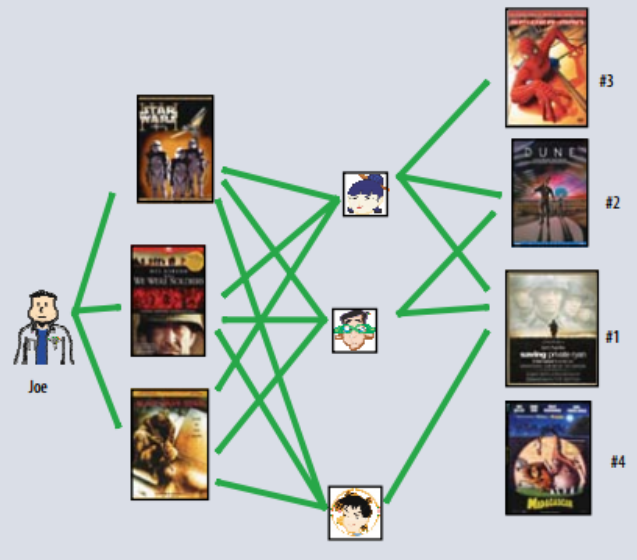
\includegraphics[width=0.7\textwidth]{cf}
	  	\caption{Filtrowanie kolaboratywne metodą sąsiedztwa,  zorientowane na użytkownika \protect\cite{koren2009matrix}.}
	  	\label{fig:cf}
	  \end{figure}
	  
	  Filtrowanie w~oparciu o~regułę sąsiedztwa koncentruje się na związkach element\-/element bądź użytkownik\-/użytkownik \cite{id:AdvancesInCollaborativeFiltering}.
	  Rysunek \ref{fig:cf} pokazuje regułę sąsiedztwa skoncentrowaną na relacji użytkownik-użytkownik. Joe ocenił trzy filmy. System odnajduje innych użytkowników, którzy ocenili te trzy pozycje podobnie jak Joe. Każdy z~nich pozytywnie ocenił film ,,Saving Private Ryan", zatem jest to pierwsza rekomendacja dla Joe. 
	  
	  \begin{figure}[!ht] 
	  	\centering
	  	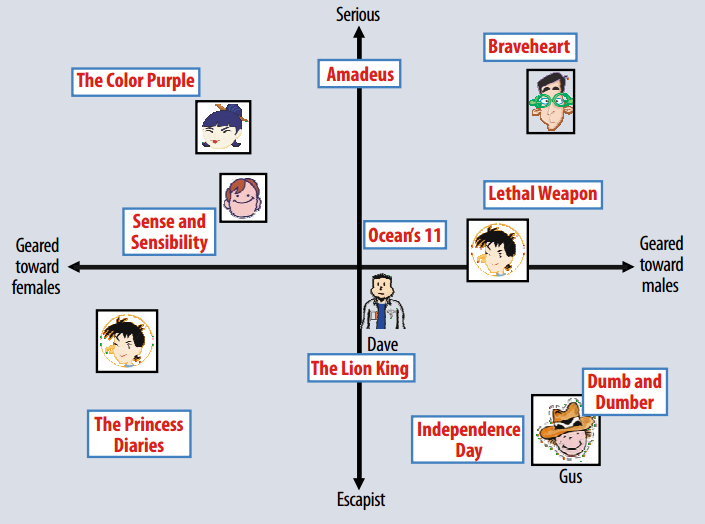
\includegraphics[width=0.7\textwidth]{cf2}
	  	\caption{Filtrowanie kolaboratywne z~wykorzystaniem modelu ukrytych parametrów \protect\cite{koren2009matrix}.}
	  	\label{fig:cf2}
	  \end{figure}
	  
	  Ideą podejścia w~oparciu o~model jest zbadanie i~modelowanie zależności element\-/użytkownik wraz z~czynnikami reprezentującymi ukryte własności elementów i~użytkowników. Taki model jest następnie uczony przy użyciu dostępnych danych. W~rezultacie można z~niego odczytać przewidywaną ocenę elementu dla konkretnego użytkownika \cite{id:ComprehensiveSurveyOfNeighborhoodBasedRecommendationMethods, id:AdvancesInCollaborativeFiltering}.
	  
	  Rysunek \ref{fig:cf2} pokazuje w~sposób uproszczony podejście oparte o~model. W~układzie współrzędnym oznaczeni są użytkownicy wedle swoich preferencji oraz konkretnych cech (np. płeć) a~także filmy, które stanowią odpowiedź na dany zestaw preferencji/cech \cite{koren2009matrix}. 
	  
	  \subsection{Zalety filtrowania kolaboratywnego}
	  
	  Filtrowanie kolaboratywne dobrze radzi sobie nawet w~wypadkach, gdzie elementy nie są dobrze opisane lub nie zawierają żadnych właściwości. Niektóre systemy zawierają treść trudną do przeanalizowania przez komputer, np. opinie, pomysły, komentarze. Mimo tego, dzięki filtrowaniu kolaboratywnemu można zbudować efektywny system rekomendacji \cite{melville2002content}.
	  
	  Dzięki zastosowaniu tej metody mniej prawdopodobne jest wystąpienia zjawiska zwanego ''bańką informacyjną'' (ang. \textit{filter bubble}). Polega ono na tym, że użytkownik otrzymując informacje wyselekcjonowane przez określony algorytm zostaje zamknięty w~pewnego rodzaju ,,bańce'', tzn. sugerowane mu elementy są do siebie podobne, gdyż dobierane są w~oparciu o~jego przeszłe zainteresowania \cite{pariser2011filter}. Dzięki filtrowaniu kolaboratywnemu użytkownik może otrzymać zaskakujące rekomendacje i~(w~zależności od domeny) odkryć nowy gatunek muzyczny, nowego reżysera lub nową kategorię produktów w~sklepie.	 
	  
	  \subsection{Wady filtrowania kolaboratywnego}
	  
	  Jednym z~problemów klasycznego podejścia do kolaboratywnego filtrowania jest brak uwzględnienia dynamiki zmian w~gustach użytkowników. Ten sam użytkownik na przestrzeni kilku lat lub miesięcy może zupełnie inaczej ocenić ten sam film bądź piosenkę. Rozwiązaniem jest dodanie czynnika czasu podczas obliczania wag kolejnych ocen. \cite{id:NewRecommentationAlgoritmBasedOnSocialNetwork,id:NextSongRecommendationWithTemporalDynamics,koren2009matrix}.
	  
	  Innym problemem jest tzw. zimny start (ang. \textit{cold start}). Polega on na tym, że nowi użytkownicy w~systemie ocenili zbyt mało elementów, aby można było zbudować dla nich dobre rekomendacje \cite{id:RubensRecSysHB2010,id:zhang2015hybrid}.
	  
	  Powszechnym zjawiskiem jest tzw. efekt długiego ogona. Rysunek \ref{fig:longtail} przedstawia jak rozkłada się procentowa ilość ocen danych elementów w~zależności od ich popularności. Jeżeli algorytm rekomendacji nie wspiera mniej popularnych elementów, to istnieje ryzyko, że użytkownicy nie otrzymają możliwości eksplorowania nowych, niszowych materiałów \cite{id:celma2010music,id:RubensRecSysHB2010}.
	  
	  \begin{figure}[!ht] 
	  	\centering
	  	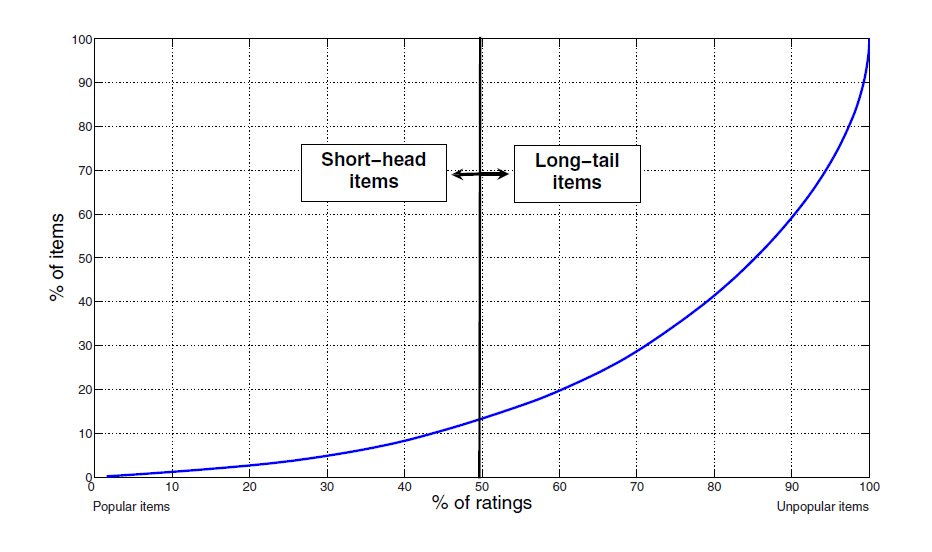
\includegraphics[width=0.7\textwidth]{longtail}
	  	\caption{Problem długiego ogona: 50\% ocen dotyczy 10-12\% najpopularniejszych elementów w~systemie \protect\cite{id:RubensRecSysHB2010}.}
	  	\label{fig:longtail}
	  \end{figure}
	  
	  Systemy rekomendacji wykorzystujące filtrowanie kolaboratywne nie są skalowalne. Złożoność rośnie proporcjonalnie do ilości użytkowników i~elementów. Wielkie koncerny internetowe takie jak Twitter wykorzystają klastry i~maszyny z~bardzo dużą pamięcią aby zachować płynność działania serwisu \cite{id:gupta2013wtf}.
	 
	 \subsection{Algorytmy filtrowania kolaboratywnego}
	 
	 Istnieje wiele implementacji algorytmów filtrowania kolaboratywnego. Jedną z~bibliotek, która takie algorytmy implementuje i~która została wykorzystana w~tym projekcie jako baza do algorytmów hybrydowych jest MyMediaLite \cite{mymedialite,gantner2011mymedialite}. Zawiera ona zestaw metod opartych zarówno o~model jak też o~regułę sąsiedztwa:
	 
	 \begin{itemize}
	 	\item SVD++ \cite{koren2008factorization}
	 	\item Biased Matrix Factorization \cite{salakhutdinov2011probabilistic,rendle2008online}
	 	\item Matrix Factorization
	 	\item Factor-Wise Matrix Factorization \cite{bell2007modeling}
	 	\item Slope One \cite{lemire2005slope}
	 	\item User-Item Baseline \cite{koren2010factor}
	 \end{itemize}
	 
	 \begin{figure}[!ht] 
	 	\centering
	 	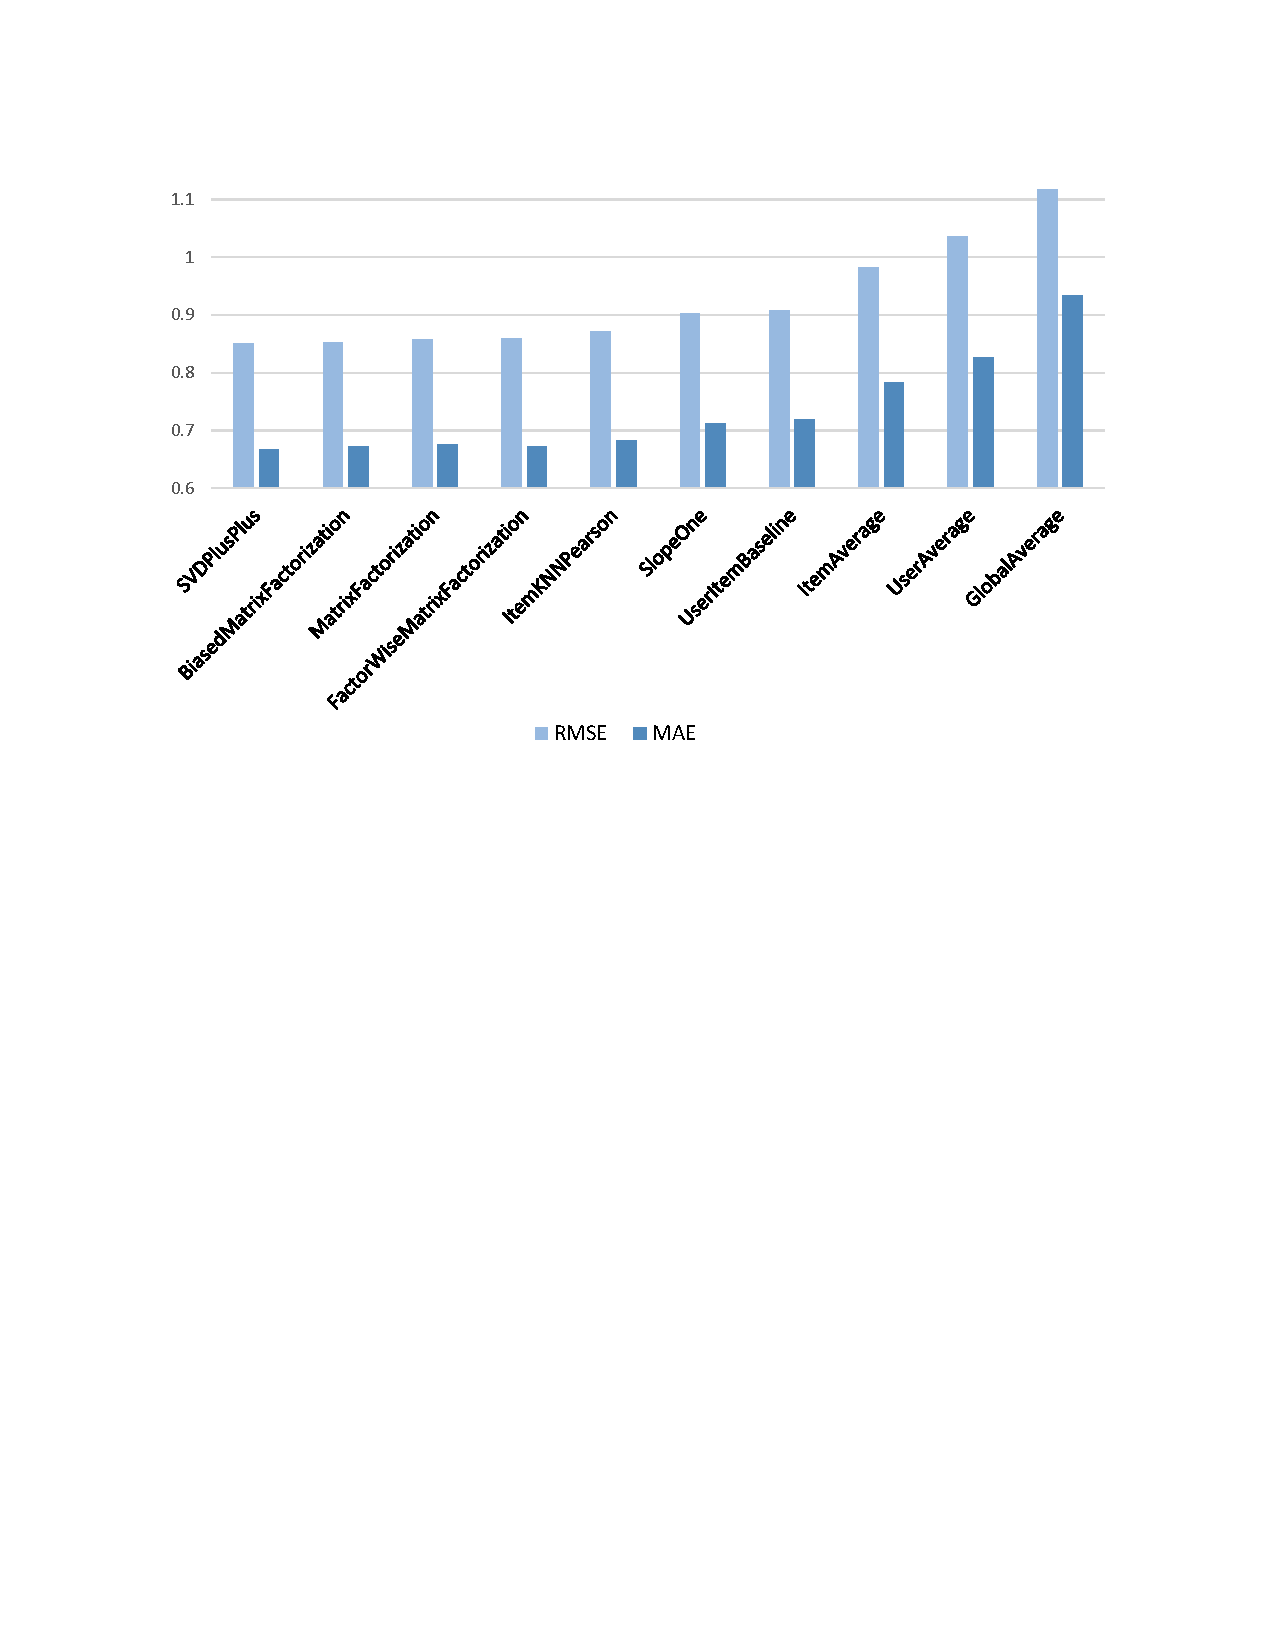
\includegraphics[width=0.7\textwidth]{cfcomparision}
	 	\caption{Test algorytmów filtrowania kolaboratywnego \protect\cite{mymedialitedatasets}}
	 	\label{fig:cfcomparision}
	 \end{figure}
	 
	 Rys. \ref{fig:cfcomparision} przedstawia wyniki działania wymienionych algorytmów (im mniejsza wartość RMSE i~MAE tym lepiej). Testy przeprowadzone zostały na bazie MovieLens M1 z~pięciokrotną walidacją krzyżową \cite{harper2016movielens}. Najefektywniejsze okazały się algorytmy SVD++, Biased Matrix Factorization i~Matrix Factorization działające w~oparciu o~model.
	 
	 \subsubsection{Matrix Factorization}	
	 
	 Algorytm \textit{Matrix Factorization} bazuje na matematycznej metodzie rozkładu macierzy na czynniki.
	 
	 
	 \begin{figure}[!ht] 
	 	\centering
	 	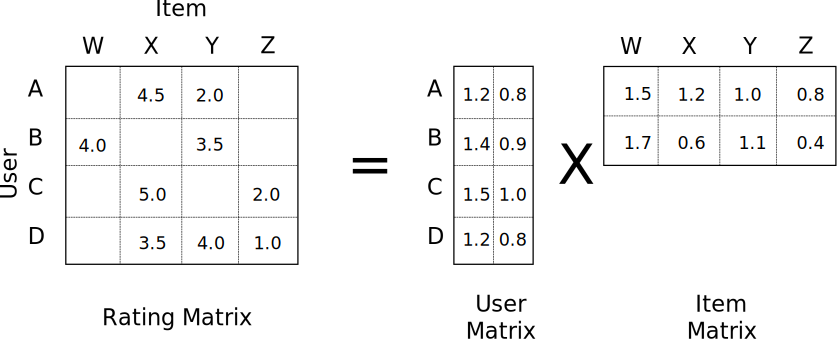
\includegraphics[width=1\textwidth]{factorization}
	 	\caption{Faktoryzacja macierzy \protect\cite{id:ComputingRecommendationsExtremeScaleApacheFlink}}
	 	\label{fig:factorization}
	 \end{figure}
	 
	 Początkowo dana jest niekompletna macierz zawierająca oceny, jakie użytkownicy wystawili konkretnym elementom (\textit{Rating Matrix}). Celem metody jest odnalezienie wartości, jakie można wstawić w~puste miejsca, czyli przewidzenie jaką ocenę dany użytkownik wystawi nieocenionemu jeszcze elementowi. 		
	 
	 w~tym celu tworzone są odrębne macierze dla użytkowników i~elementów zawierające ukryte własności. Każdy element powiązany jest z~wektorem $q_i \in \mathbb{R} ^f$ (wektory W, X, Y, z~na rys. \ref{fig:factorization}) a~każdy użytkownik z~wektorem $p_u \in \mathbb{R} ^f$ (wektory A, B, C, D na rys. \ref{fig:factorization}). Wartości czynników ukrytych determinują stopień zainteresowania daną cechą (w~przypadku macierzy użytkowników) bądź stopień, w~jakim dany element posiada tę cechę (w~przypadku macierzy elementów).		
	 
	 Iloczyn skalarny $q_i^T p_u$ przedstawia relację pomiędzy użytkownikiem a~elementem. Na tej podstawie można wnioskować ocenę $r_{ui}$, jaką użytkownik może wystawić elementowi: $r_{ui} = q_i^T p_u$ i~w konsekwencji estymować zainteresowanie użytkownika danym elementem \cite{koren2009matrix}.
	 
	 Głównym wyzwaniem jest odnalezienie wartości macierzy użytkownika i~elementu, które po przemnożeniu przez siebie dadzą kompletną macierz ocen. W~przypadku omawianych algorytmów stosowana jest metoda stochastycznego gradientu prostego. 
	 
	 \subsubsection{Stochastyczny gradient prosty}
	 
	 Stochastyczny gradient prosty (ang. \textit{stochastic gradient descent}, \textit{SGD}) jest iteracyjnym algorytmem optymalizacyjnym mającym za zadanie odnalezienie minimum bądź maksimum zadanej funkcji. Jest on uproszczeniem popularnej metody gradientu prostego \cite{bottou2012stochastic}.
	 
	 Dana jest funkcja celu w~postaci
	 
	 \begin{equation}
	 \label{eq:sgd1}
	 Q(w) = \sum_{i=1}^{n}Q_i(w)
	 \,.
	 \end{equation}			
	 Zadaniem algorytmu jest odnalezienie takiej wartości parametru $w$, dla którego $Q(w)$ będzie minimalne. Wykorzystując klasyczną metodę gradientu prostego poszukiwania można zapisać następującym wzorem:
	 
	 \begin{equation}
	 \label{eq:sgd2}
	 w:= w~- \eta \sum_{i=1}^{n} \nabla Q_i(w)
	 \,,
	 \end{equation}			
	 gdzie $\eta$ symbolizuje współczynnik uczenia (ang. \textit{learning rate}). W~przypadku algorytmu stochastycznego następuje uproszczenie. Zamiast obliczać dokładny gradient $Q(w)$, w~każdej iteracji jest  on aproksymowany na podstawie pojedynczego, losowo wybranego przypadku:
	 
	 \begin{equation}
	 \label{eq:sgd3}
	 w:= w~- \eta \nabla Q_i(w)
	 \,.
	 \end{equation}			
	 Algorytm przetwarza wszystkie elementy zbioru treningowego i~dla każdego przypadku wykonuje aktualizację wartości $w$. Przebieg algorytmu przedstawiony jest poniżej (algorytm \ref{aq:sgd}).
	 
	 \def\alghoritm5{Stochastyczny gradient prosty}
	 \begin{breakablealgorithm}
	 	\caption{\alghoritm5}
	 	\myalgorithm{\alghoritm5}
	 	\label{aq:sgd}
	 	\begin{algorithmic}
	 		\STATE $w \leftarrow \text{początkowy wektor } w$
	 		\STATE $\eta \leftarrow \text{współczynnik uczenia}$
	 		
	 		\WHILE{nie odnaleziono minimum}
	 		
	 		\STATE losowo mieszaj przykłady ze zbioru testowego
	 		\FOR {$i \in \{1, 2, \ldots, n\} $}
	 		\STATE $w:= w~- \eta \nabla Q_i(w)$
	 		\ENDFOR
	 		\ENDWHILE
	 	\end{algorithmic}
	 \end{breakablealgorithm}
	 
	 Stochastyczny gradient prosty wykonuje dużo więcej kroków niż jego klasyczny odpowiednik aby odnaleźć rozwiązanie optymalne. Mimo tego jest on szybszy, gdyż każdy pojedynczy krok jest mniej kosztowny niż w~oryginale. Różnicę w~działaniu przedstawia rys. \ref{fig:sgd}.  
	 
	 \begin{figure}[!ht] 	
	 	\centering	 		 	
	 	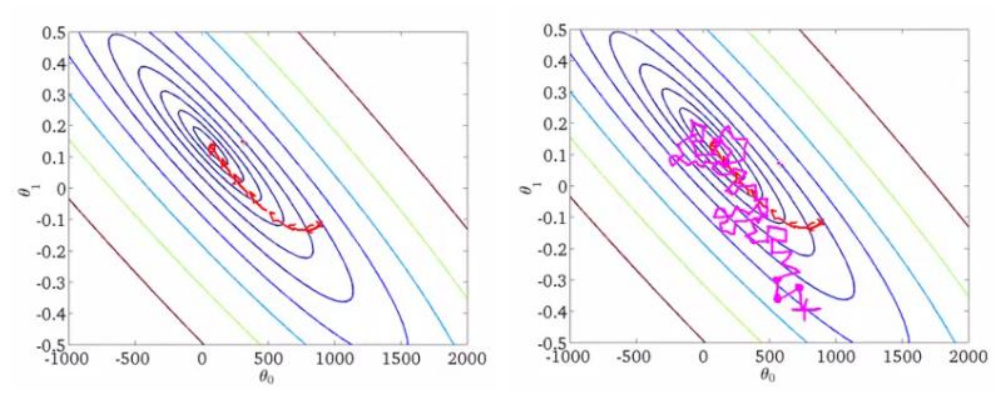
\includegraphics[width=0.5\textwidth]{sdg}
	 	\caption{Różnica pomiędzy klasycznym gradientem prostym (po lewej) a~jego stochastyczną wersją (po prawej) \protect\cite{effandpractstochsub}}
	 	\label{fig:sgd}
	 \end{figure}
	 
	 \newpage
	 \subsubsection{Przebieg algorytmu Matrix Factorization}
	 
	 Przebieg algorytmu składa się z~dwóch faz. W~pierwszej fazie inicjowany jest model (zob. algorytm \ref{aq:mf_init}). Daną wejściową jest macierz zawierająca dotychczasowe oceny  elementów przez użytkowników w~systemie. Na wyjściu otrzymywane są dwie nowe macierze reprezentujące ukryte własności użytkowników i~elementów. Na tym etapie są one wypełnione wartościami losowymi w~celu ułatwienia kolejnych obliczeń. W~następnych etapach algorytmu wartości te zostaną zamienione tak, że reprezentować będą rzeczywistą relację pomiędzy elementem i~użytkownikiem.
	 
	 
	 \def\alghoritm1{Matrix Factorization -- Inicjacja modelu}
	 \begin{breakablealgorithm}
	 	\caption{\alghoritm1}
	 	\myalgorithm{\alghoritm1}
	 	\label{aq:mf_init}
	 	\begin{algorithmic}
	 		\STATE $N \leftarrow $ liczba użytkowników
	 		\STATE $M \leftarrow $ liczba elementów
	 		\STATE $F \leftarrow $ liczba ukrytych własności
	 		\STATE $ratings \leftarrow $ Macierz NxM zawierająca dotychczasowe oceny wszystkich elementów
	 		\STATE przez wszystkich użytkowników
	 		\STATE $user\_factors \leftarrow $ Macierz NxF reprezentująca ukryte własności użytkowników
	 		\STATE $item\_factors \leftarrow $ Macierz MxF reprezentująca ukryte własności elementów
	 		
	 		\FOR{each $uf \in user\_factors$, $if \in item\_factors$ }
	 		\STATE wstaw losową wartość za pomocą transformacji Boxa--Mullera
	 		\ENDFOR
	 		
	 		\FOR{each $user, item \in ratings$ }			
	 		\IF {$ratings_{user,item} = NULL$}
	 		\STATE wstaw 0 do wiersza $user\_factors_{user}$ i~$item\_factors_{item}$
	 		\ENDIF				
	 		\ENDFOR
	 		\RETURN $user\_factors, item\_factors$
	 	\end{algorithmic}
	 \end{breakablealgorithm}
	 
	 
	 w~fazie drugiej następuje uczenie metodą stochastycznego gradientu prostego (zob. algorytm  \ref{aq:mf_learn}). Wynikiem tej fazy są macierze reprezentujące ukryte własności użytkowników i~elementów. Mnożąc je ze sobą uzyskiwana jest przewidywana ocena każdego z~elementów przez użytkowników. 
	 
	 Przed rozpoczęciem uczenia ustalane są parametry: parametr regulujący (ang. \textit{regularization}), współczynnik uczenia (ang. \textit{learning rate}), parametr zanikania (ang. \textit{decay}) i~liczba iteracji. 	
	 w~trakcie trwania głównej pętli parametr regulujący pozostaje niezmienny. Służy on zapobieganiu zjawisku nadmiernego dopasowania (ang. \textit{overfitting}). Tempo uczenia jest przy każdym przebiegu pętli mnożone przez parametr zanikania, dzięki czemu można kontrolować w~jakim stopniu kolejne przebiegi pętli wpływają na finalny wynik. 
	 
	 Ostatnim parametrem ustalanym przed główną pętlą jest skośność globalna (ang. \textit{global bias}), która jest średnią wszystkich znanych ocen. 
	 
	 w~pętli uczenia wykonywane są następujące operacje: dla każdej pary użytkownik\-/element budowana jest przewidywana ocena poprzez obliczenie iloczynu skalarnego odpowiednich wartości z~macierzy wartości ukrytych. Ocena ta jest modyfikowana poprzez dodanie globalnej skośności a~następnie porównywana z~faktyczną oceną elementu przez użytkownika. Tak uzyskany błąd służy do wyliczenia delty. Macierze wartości ukrytych uaktualniane są o~wyliczoną deltę. 
	 
	 Pod koniec każdej iteracji aktualizowany jest współczynnik uczenia.
	 
	 \def\alghoritm2{Matrix Factorization -- Faza uczenia}
	 \begin{breakablealgorithm}
	 	\caption{\alghoritm2}
	 	\myalgorithm{\alghoritm2}
	 	\label{aq:mf_learn}
	 	\begin{algorithmic}
	 		\STATE $global\_bias \leftarrow $ średnia wszystkich ocen
	 		\STATE $X \leftarrow $ liczba iteracji			
	 		\STATE $regularization \leftarrow $ parametr regulujący			
	 		\STATE $current\_learnrate \leftarrow $ współczynnik uczenia
	 		\STATE $decay \leftarrow $ parametr zanikania
	 		
	 		\FOR{each $x \in X$ }
	 		\FOR{each $user, item \in ratings$ }
	 		
	 		\STATE $predicion= global\_bias + IloczynSkalarny(user\_factors_{user}, item\_factors_{item}); $
	 		
	 		\STATE $error = ratings_{user,item} - prediction$
	 		
	 		\textbf{//dopasowanie własności ukrytych:}
	 		
	 		\FOR{each $f \in F$}
	 		\STATE $delta_u = error * item\_factors_{item, f} - regularization * user\_factors_{user, f}$
	 		\STATE $delta_i = error * user\_factors_{user, f} - regularization * item\_factors_{item, f}$
	 		
	 		\STATE $user\_factors_{user, f} \incr current\_learnrate * delta_u$
	 		\STATE $item\_factors_{item, f} \incr current\_learnrate * delta_i$
	 		\ENDFOR					
	 		\ENDFOR			
	 		\STATE $current\_learnrate \incrtimes decay$				
	 		\ENDFOR
	 		\RETURN $user\_factors, item\_factors$
	 	\end{algorithmic}
	 \end{breakablealgorithm}
	 
	 
	 \subsubsection{Biased Matrix Factorization}
	 
	 Algorytm \textit{Biased Matrix Factorization} jest modyfikacją wyżej opisanego algorytmu \textit{Matrix Factorization}. Podobnie jak jego pierwowzór składa się z~dwóch faz. W~pierwszej fazie dodatkowo inicjowane są dwa dodatkowe wektory: skośność użytkowników (ang. \textit{user bias}) i~skośność elementów (ang. \textit{item bias}). 
	 
	 Inaczej jest też obliczana skośność globalna: 
	 
	 \begin{equation}
	 \label{eq:global_bias}
	 global\_bias = 
	 \frac
	 { 
	 	\frac{ a - r_{min} }{ r_{max} - r_{min} }
	 }
	 {
	 	1 - \frac{ a - r_{min} }{ r_{max} - r_{min} }	
	 }
	 \,,
	 \end{equation} 		 		
	 gdzie
	 
	 \begin{conditions*}
	 	a & to średnia wszystkich ocen \\
	 	r_{min}  &  to minimalna ocena w~systemie  \\
	 	r_{max}  &  to maksymalna ocena w~systemie
	 \end{conditions*} 
	 
	 Faza druga wygląda podobnie jak w~przypadku algorytmu \textit{Matrix Factorization}, jednak są uwzględniane dodatkowe parametry i~wykonywane dodatkowe kroki.
	 
	 \def\alghoritm3{Biased Matrix Factorization -- Faza uczenia}
	 \begin{breakablealgorithm}
	 	\caption{\alghoritm3}
	 	\myalgorithm{\alghoritm3}
	 	\label{aq:bmf_learn}
	 	\begin{algorithmic}
	 		\STATE $global\_bias \leftarrow $ średnia wszystkich ocen
	 		\STATE $X \leftarrow $ liczba iteracji			
	 		\STATE $regU, regI, BiasReg \leftarrow $ parametry regulujące dla użytkownika, elementu i~ogólny 			
	 		\STATE $current\_learnrate \leftarrow $ współczynnik uczenia
	 		\STATE $BiasLearnRate \leftarrow $ współczynnik uczenia skośności
	 		\STATE $decay \leftarrow $ parametr zanikania
	 		
	 		\FOR{each $x \in X$ }
	 		\FOR{each $user, item \in ratings$ }			 		
	 		\STATE $score= global\_bias + user\_bias_{user} + item\_bias_{item} + IloczynSkalarny(user\_factors_{user}, item\_factors_{item})$
	 		
	 		\STATE $sig\_score = \frac{1}{1 + \exp(-score)}$
	 		
	 		\STATE $predicion= rating_{min} + sig\_score + (rating_{max} - rating_{min}) $
	 		
	 		\STATE $error = ratings_{user,item} - prediction$
	 		
	 		\STATE $gradient\_common = err * sig\_score * (1 - sig\_score) * (rating_{max} - rating_{min})$
	 		
	 		\textbf{//dopasowanie skośności:}
	 		
	 		\STATE $user\_bias_{user} \incr BiasLearnRate * current\_learnrate * (gradient\_common - BiasReg * RegU * user\_bias_{user})$
	 		
	 		\STATE $item\_bias_{item} \incr BiasLearnRate * current\_learnrate * (gradient\_common - BiasReg * RegI * item\_bias_{item})$
	 		
	 		\textbf{//dopasowanie własności ukrytych:}
	 		
	 		\FOR{each $f \in F$}
	 		\STATE $delta_u = gradient\_common * item\_factors_{item, f} - RegU * user\_factors_{user, f}$
	 		
	 		\STATE $delta_i = gradient\_common * user\_factors_{user, f} - RegI * item\_factors_{item, f}$
	 		
	 		\STATE $user\_factors_{user, f} \incr current\_learnrate * delta_u$
	 		\STATE $item\_factors_{item, f} \incr current\_learnrate * delta_i$
	 		\ENDFOR					
	 		\ENDFOR			
	 		\STATE $current\_learnrate \incrtimes decay$				
	 		\ENDFOR
	 		\RETURN $user\_factors, item\_factors$
	 	\end{algorithmic}
	 \end{breakablealgorithm}
	 
	 \subsubsection{SVD++}
	 
	 SVD++ jest rozszerzeniem metody SVD (dekompozycja głównych składowych, ang. \textit{singular value decomposition}). Od poprzednich omawianych algorytmów różni go przede wszystkim to, że korzysta nie tylko z~bezpośredniej informacji zwrotnej do tworzenia profilu użytkownika ale także z~pośredniej (zob. \ref{ss:metody_tworzenia_profilu_uzytkownika}).
	 
	 Model SVD++ opisywany jest równaniem:
	 
	 \begin{equation}
	 \label{eq:svd}
	 r_{ui} = \mu + b_u + b_i + q_i^T (p_u + \frac{1}{\sqrt{|N(u)|}} \sum_{j \in N(u)}^{} y_j) 
	 \,
	 \end{equation}		 		 
	 Użytkownik powiązany jest z~wektorem $p_u \in \mathbb{R} ^f$ reprezentującym zainteresowanie konkretnymi cechami. Taki model uzupełniany jest sumą  $\frac{1}{\sqrt{|N(u)|}} \sum_{j \in N(u)}^{} y_j$, która reprezentuje pośrednie informacje zwrotne. Przykładem informacji niejawnej jest fakt, że użytkownik w~ogóle zareagował na dany element (np. ocenił go), bez względu na wynik tej interakcji. 
	 
	 Zmienne $b_u$ i~$b_i$ reprezentują obserwowane odchylenie od średniej dla użytkowników i~elementów, natomiast $\mu$ to średnia wszystkich ocen \cite{koren2008factorization}. 
	 
	 \section{Filtrowanie z~analizą zawartości}
	 \label{s:filtrowaniezanalizazawartosci}
	 
	 Filtrowanie z~analizą zawartości opiera się na cechach elementów w~systemie. Rekomendowane są obiekty, które podobne są do tych pozytywnie ocenionych wcześniej przez użytkownika \cite{id:huynh2012modeling}. W~zależności od domeny pod uwagę mogą być brane słowa kluczowe, cechy takie jak rok wydania, reżyser, autor, kompozytor, gatunek itp.
	 
	 \subsection{Zalety filtrowania z~analizą zawartości}
	 
	 Do zalet filtrowania z~analizą zawartości należy niezależność użytkownika. Podczas budowania rekomendacji brany pod uwagę jest tylko jego profil, aktywność innych aktorów w~systemie nie wpływa na wynik końcowy. Nawet, gdy w~bazie będzie istniało niewielu użytkowników lub ocenią oni zupełnie inne elementy niż użytkownik aktywny, to rekomendacja w~dalszym ciągu może być miarodajna. 
	 
	 Inną przewagą jest przejrzystość -- każda propozycja jest w~pełni uzasadniona, gdyż opiera się na działaniach użytkownika w~przeszłości. Ponadto, tego typu algorytm ma możliwość zaproponowania elementu, który nie był nigdy wcześniej oceniany przez nikogo. Zapobiega to zjawisku długiego ogona \cite{id:ContentBasedRecommenderSystemsState}.
	 
	 \subsection{Wady filtrowania z~analizą zawartości}
	 Aby rekomendacja była skuteczna użytkownik powinien ocenić jak najwięcej elementów. Problematyczni są zatem użytkownicy, którzy dopiero co dołączyli do serwisu oraz tacy, którzy nie są aktywni i~rzadko zostawiają po sobie ślad \cite{id:MaleszkaMianowskaNguyenmethod}.
	 
	 Filtrowanie z~analizą zawartości jest podatne na pułapkę tzw. bańki informacyjnej. Jeżeli w~systemie rekomendującym produkcje kinowe użytkownik do tej pory oceniał jedynie filmy akcji, to mało prawdopodobne jest, że algorytm zaproponuje mu ciekawy dramat obyczajowy. Nowe propozycje nie są zaskakujące \cite{id:ContentBasedRecommenderSystemsState}.
	 	 
	 \subsection{Metody tworzenia profilu użytkownika}
	 \label{ss:metody_tworzenia_profilu_uzytkownika}
	 
	 Profil użytkownika może być tworzony na dwa sposoby. Jeżeli użytkownik jawnie pozostawia informacje można mówić bezpośredniej informacji zwrotnej (ang. \textit{explicit feedback}). Do takich informacji należą: ocena konkretnych elementów, przycisk lubienia lub nielubienia (tzw. ,,łapka'' w~górę lub w~dół), komentarz itp. 
	 
	 Gdy użytkownik nie zostawia po sobie tego typu śladów, to informacje na temat jego zachowań i~preferencji można uzyskać korzystając z~pośredniej informacji zwrotnej (ang. \textit{implicit feedback}). System bierze wówczas pod uwagę aktywność użytkownika taką jak: historia zakupów, historia przeglądarki a~nawet ruchy myszką. W~przypadku serwisu z~muzyką czy filmem pośrednią informacją zwrotną będzie fakt, czy użytkownik wysłuchał lub obejrzał dany materiał do końca czy też wyłączył go po paru sekundach \cite{id:AdvancesInCollaborativeFiltering,id:ContentBasedRecommenderSystemsState}.
	 
	 \subsection{Algorytmy wykorzystywane w~implementacji filtrowania z~analizą zawartości}
	 
	 Najprostszym sposobem implementacji filtrowania z~analizą zawartości jest wyciąganie średnich wartości cech z~wektora ocenianego elementu. Bardziej efektywne jest jednak wykorzystanie technik uczenia maszynowego takich jak naiwny klasyfikator bayesowski, klasteryzacja, drzewa decyzyjne lub sztuczne sieci neuronowe. W~niniejszej pracy wykorzystana została sztuczna sieć neuronowa uczona algorytmami opisanymi poniżej. 
	 
	 \subsubsection{Propagacja wsteczna}
	 \label{sss:backprop}
	 
	 Algorytm propagacji wstecznej jest jedną z~popularniejszych metod uczenia nadzorowanego jednokierunkowych sieci neuronowych. Zbiór uczący składa się z~danych wejściowych (wektory cech elementu) i~z informacji o~oczekiwanym wyniku (ocena elementu). Różnica między wynikiem zwróconym przez sieć a~wartością oczekiwaną stanowi miarę błędu sieci neuronowej. 
	 
	 \begin{figure}[!ht] 
			 	\centering
			 	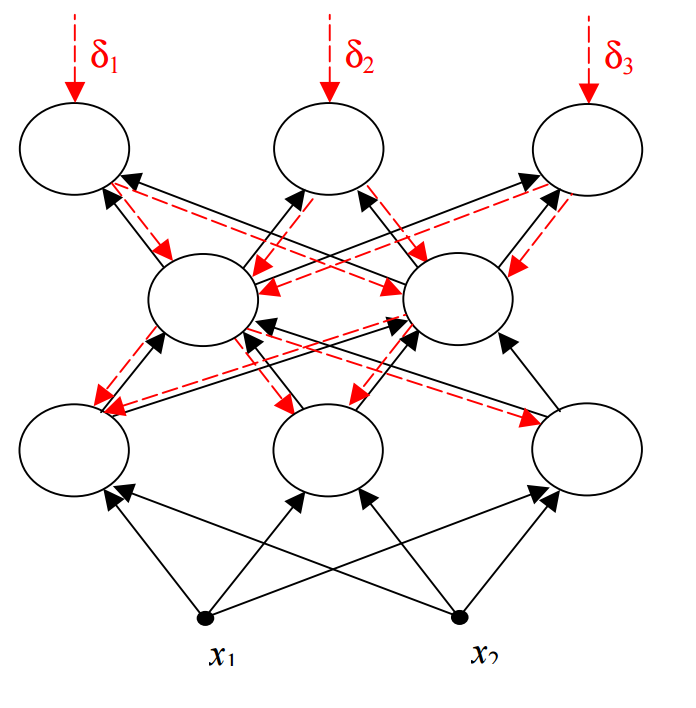
\includegraphics[width=0.5\textwidth]{ilustracjabackprop}
			 	\caption{Algorytm propagacji wstecznej w~sieci trójwarstwowej -- idea działania \protect\cite{kwateralgorytmy}}
			 	\label{fig:ilustracjabackprop}
	 \end{figure}
	 
	 Wiadomo, że funkcja celu jest funkcją ciągłą. Bazując na gradientowych metodach optymalizacji, wagi w~sieci neuronowej aktualizowane są w~następujący sposób:	 
	 
	 \begin{equation}
	 \label{eq:weightadaptation3}
	 W_{ij}(n+1) = W_{ij}(n) + \Delta W_{ij}(n) 
	 \,,
	 \end{equation}
	 
	 
	 \begin{equation}
	 \label{eq:weightadaptation2}
	 \Delta W_{ij}(n) = \eta p(W)
	 \,,
	 \end{equation}		 
	 gdzie
	 
	 \begin{conditions*}
			 	\eta & to współczynnik uczenia (ang. \textit{learning rate}) \\
			 	p(W) & to kierunek w~przestrzeni wielowymiarowej W~
	 \end{conditions*} 
	 
	 Aby wyznaczyć kierunek $p(W))$ dla wszystkich warstw sieci należy przejść przez kolejne etapy uczenia \cite{haykin1994neural,hertz1993wstkep,kwateralgorytmy,osowski1996sieci,timothy1996sieci}.
	 
	 \begin{enumerate}
			 	\item W~kroku pierwszym sieć neuronowa poddawana jest analizie o~zwykłym kierunku przepływu sygnałów. Wynikiem są wartości sygnałów wychodzących z~neuronów warstw wyjściowej i~ukrytych oraz pochodne funkcji aktywacji w~kolejnych warstwach. 
			 	
			 	\item W~kroku drugim kierunek przepływu sygnałów zostaje odwrócony (stąd nazwa propagacja wsteczna). Funkcje aktywacji zostają zastąpione przez swoje pochodne. Na oryginalne wyjście sieci (aktualnie wejście) podana zostaje wartość równa różnicy pomiędzy wynikiem oczekiwanym a~wynikiem zwróconym przez sieć. 
			 	
			 	\item Obliczana zostaje wartość różnic wstecznych.
			 	
			 	\item W~kolejnym kroku następuje wreszcie proces adaptacji wag. Odbywa się on zarówno dla sieci zwykłej jak i~dla sieci o~propagacji wstecznej. Reguła modyfikacji ma postać: 
			 	
			 	\begin{equation}
			 	\label{eq:weightadaptation4}
			 	\Delta W_{ij} = \eta \sum_\text{wzroce}^{} \delta_\text{wyjście} \cdot x_\text{wejście}
			 	\,,
			 	\end{equation}
			 	
			 	\item Powyższe kroki potarzane są dla każdej pary dane wejściowe -- oczekiwany wynik tak długo, aż poziom błędu spadnie poniżej akceptowalnej wartości bądź osiągnięta zostanie maksymalna liczba iteracji. 
			 	
	 \end{enumerate}
	 
	 Algorytm propagacji wstecznej obrazuje schemat blokowy \ref{fig:propagacjawsteczna}.
	 
	 \begin{figure}[!ht] 
			 	\centering
			 	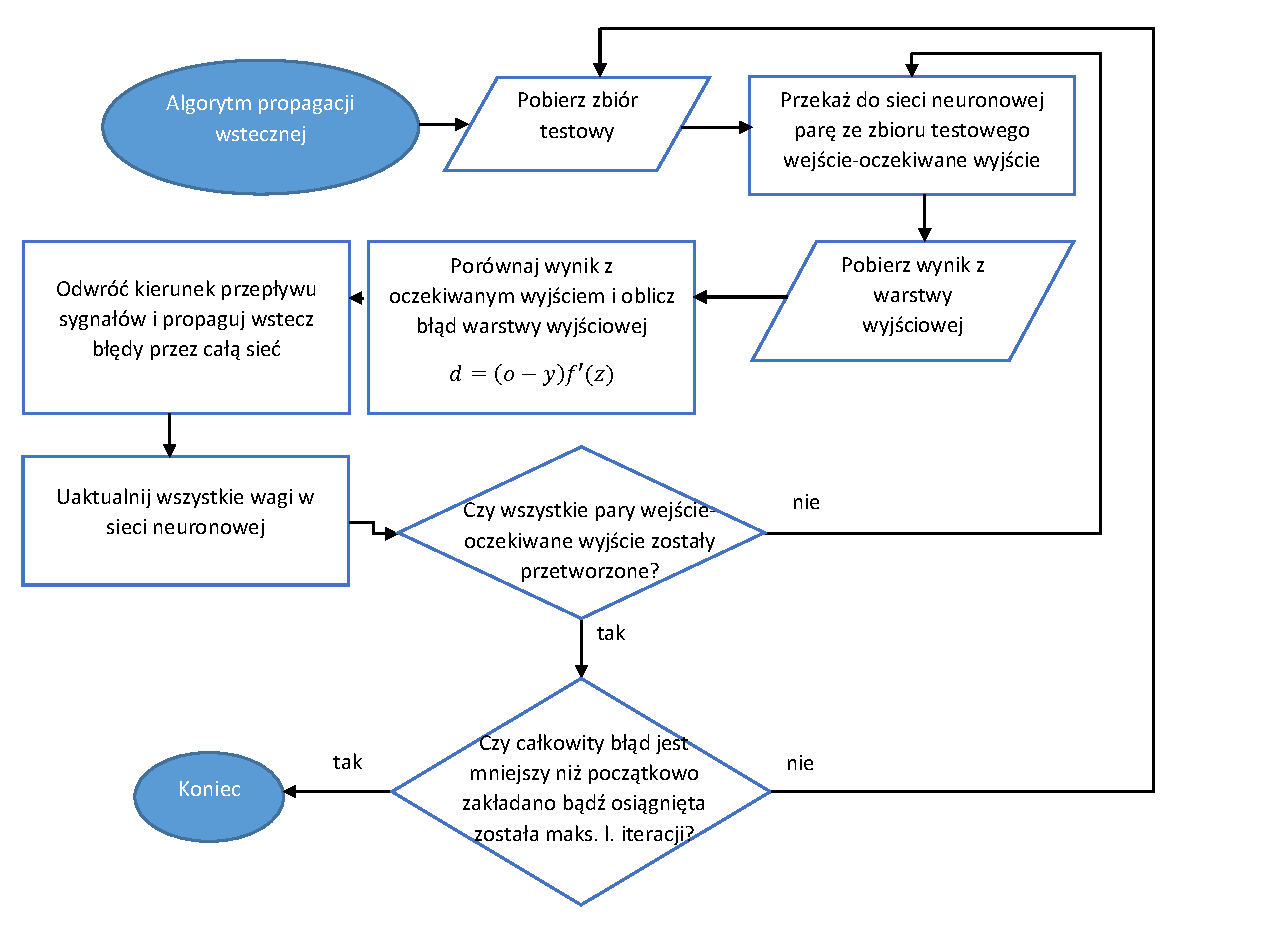
\includegraphics[width=1\textwidth]{propagacjawsteczna}
			 	\caption{Algorytm propagacji wstecznej}
			 	\label{fig:propagacjawsteczna}
	 \end{figure}
	 
	 \subsubsection{Współczynnik bezwładności}
	 \label{sss:metoda_momentum}
	 
	 W~celu zwiększenia efektywności działania algorytmu został on zmieniony poprzez dołączenie członu zwanego współczynnikiem bezwładności (momentum). Standardowy sposób aktualizacji wag sieci (równanie \ref{eq:weightadaptation3}) został zmodyfikowany w~następujący sposób:
	 
	 \begin{equation}
	 \label{eq:zasadamomentum1}
	 W_{ij}(n+1) = W_{ij}(n) + \Delta W_{ij}(n) 
	 \,,
	 \end{equation}
	 
	 \begin{equation}
	 \label{eq:zasadamomentum2}
	 \Delta W_{ij}(n) = \eta(n) \cdot p(n) + \alpha(W_{ij}(n)-W_{ij}(n-1)) 
	 \,,
	 \end{equation}		 
	 gdzie $\alpha$ jest współczynnikiem bezwładności z~zakresu $[0,1]$. Im wyższa wartość współczynnika tym większy jego wpływ na ostateczny kształt kolejnych wag. W~dalszej części pracy przeprowadzono eksperymenty mające na celu dobranie optymalnej wartości współczynnika bezwładności.
	 
	 \subsubsection{Algorytm RPROP}		 
	 
	 Pomimo dużej popularności algorytmu propagacji wstecznej nie jest on pozbawiony wad. Sporym problemem jest jego relatywnie niska szybkość działania, szczególnie w~przypadku bardzo dużych sieci neuronowych -- a~więc w~przypadku odpowiadającemu potrzebom systemów rekomendacji. W~odpowiedzi na te problemy Martin Riedmiller i~Heinrich Braun zaproponowali w~1992 roku alternatywny algorytm -- Resilient Backpropagation (RPROP).
	 
	 Główną różnicą jest wykorzystywanie jedynie informacji o~dodatniości lub ujemności każdej składowej gradientu zamiast o~ich wartości (jak to się odbywa w~oryginalnym algorytmie). Ponadto, współczynnik uczenia modyfikowany jest w~każdym kolejnym kroku. 
	 
	 Modyfikacja współczynników odbywa się zgodnie ze wzorem:
	 
	 \begin{equation}
	 \label{eq:rprop}		 
	 \eta(t) = 
	 \begin{cases}
	 min\{a \eta(t-1), \eta_{max}\}, & \quad \text{gdy } \frac{\partial E^2(t)}{\partial v(t)} \frac{\partial E^2(t-1)}{\partial v(t-1)} > 0 \\
	 max\{b \eta(t-1), \eta_{min}\}, & \quad \text{gdy } \frac{\partial E^2(t)}{\partial v(t)} \frac{\partial E^2(t-1)}{\partial v(t-1)} < 0 \\
	 \eta(n-1), & \quad \text{w każdym innym przypadku} 
	 \end{cases}		 
	 \,,
	 \end{equation}		 
	 gdzie $\frac{\partial E^2(t)}{\partial v(t)}$ jest dokładną wartością składowej $v$ gradientu. Ponadto stałe $a$, $b$, $\eta_{min}$ i~$\eta_{max}$ są zdefiniowane następująco:
	 
	 \begin{conditions*}
			 	a = 1.2 \\
			 	b = 0.5 \\
			 	\eta_{min} = 10^{-6} \\
			 	\eta_{max} = 50
	 \end{conditions*} 
	 
	 Algorytm RPROP jest efektywniejszy pod kątem prędkości działania względem tradycyjnej propagacji wstecznej, więc dobrze sprawdza się tam, gdzie szybkość jest ważniejsza od wysokiej poprawności wyników \cite{riedmiller1993direct,riedmiller1994rprop}.
	 
	 \subsubsection{Algorytm genetyczny}	
	 		 \label{ss:algorytm_genetyczny}
	 		 
	 		 Koncepcja algorytmów genetycznych została zaproponowana już 1960 roku przez Johna Hollanda. Należą one do klasy algorytmów ewolucyjnych, inspirowanych zasadą doboru naturalnego Darwina. Analogią do środowiska naturalnego jest pewien problem, dla którego poszukiwane jest optymalne rozwiązanie. Populacja składa się z~potencjalnych rozwiązań, które są oceniane funkcją przystosowania. Zgodnie z~zasadą Darwina zwycięża najsilniejszy, czyli najlepsze (chociaż nie zawsze optymalne) rozwiązanie \cite{pena2000evolutionary}. Schemat działania algorytmów genetycznych przedstawia rys. \ref{fig:algorytmgenetyczny}.	 
	 		 
	 		 
	 		 \begin{figure}[!ht] 
	 		 	\centering
	 		 	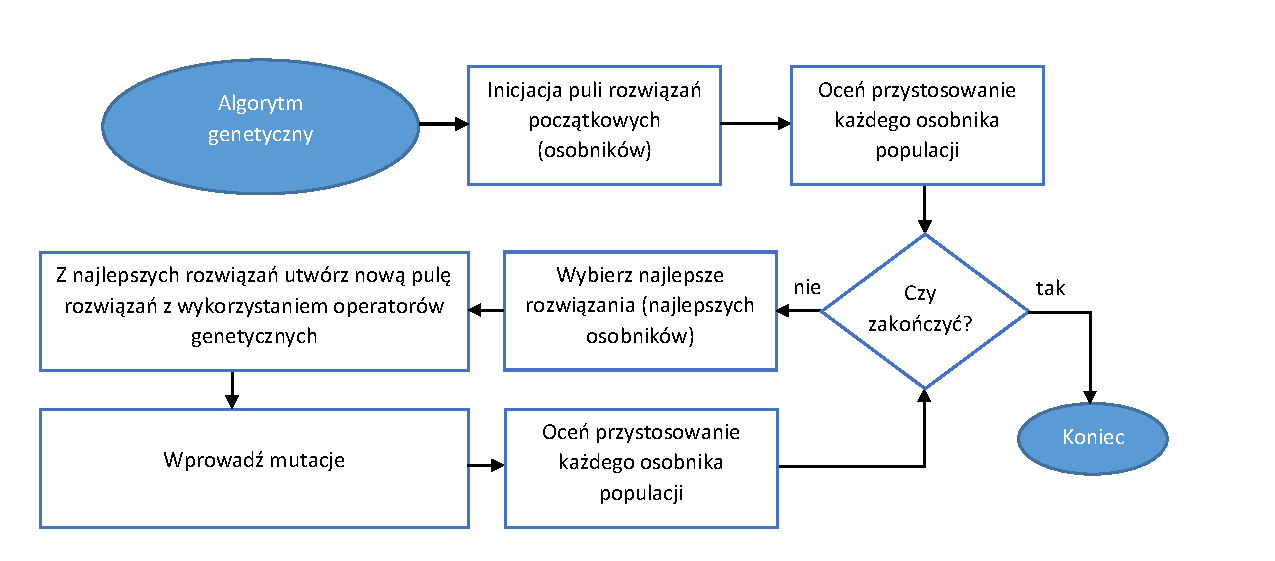
\includegraphics[width=1\textwidth]{algorytmgenetyczny}
	 		 	\caption{Ogólny schemat algorytmu genetycznego}
	 		 	\label{fig:algorytmgenetyczny}
	 		 \end{figure}
	 		 
	 		 Jako, że algorytmy genetyczne należą do grupy algorytmów optymalizacyjnych mogą zostać wykorzystane do uczenia sieci neuronowych. W~przypadku tej implementacji populację stanowią propozycje wag dla każdego perceptronu. Preferowane są takie zestawy wag, dla których sieć zwraca rezultaty obarczone najmniejszym błędem. Najlepsze zestawy są ze sobą krzyżowane oraz podlegają mutacji. W~wyniku takich mechanizmów ewolucyjnych powstaje rozwiązanie, dla których sieć neuronowa zwraca oczekiwane rezultaty \cite{aforgenetgenetic,montana1989training}.
	 		 
	 
	 \section{Algorytmy hybrydowe}
	 \label{s:algorytmyhybrydowe}

	 W~wielu przypadkach podejście hybrydowe okazuje się bardziej skuteczne niż samo filtrowanie z~analizą zawartości lub kolaboratywne. Algorytmy hybrydowe można budować na wiele różnych sposobów. Jednym z~nich jest odrębna implementacja filtrowania z~analizą zawartości i~filtrowania kolaboratywnego a~następnie łączenie ich wyników. Łączyć wyniki można poprzez liniową kombinację ocen bądź też schemat głosowania \cite{claypool1999combining}. Alternatywą jest wybór algorytmu decydującego na podstawie zadanych metryk jakości, na przykład ilości cech danego elementu bądź kompletności macierzy ocen użytkownik-element.
	 
	 Innym sposobem jest wykorzystanie charakterystyki filtrowania kolaboratywnego w~podejściu z~analizą zawartości. Pozwala ono na redukcję wymiarowości. Alternatywą jest podejście odwrotne, tzn wykorzystanie charakterystyki filtrowania z~analizą zawartości w~podejściu kolaboratywnym. Uwzględnienie profilu użytkownika i~charakterystyki elementów pozwala na pokonanie problemów związanych ze zbyt rzadkim wypełnieniem macierzy ocen użytkownik-element \cite{adomavicius2005toward}.
	 
	 Kolejnym spotykanym podejściem jest konstruowanie ogólnego, jednolitego modelu, który zawiera charakterystyki zarówno filtrowania z~analizą zawartości jak i~kolaboratywnego.
	 Przykładowo \cite{basu1998recommendation} proponuje wykorzystanie charakterystyki opartej o~zawartość i~kolaboratywnej w~pojedynczym klasyfikatorze regułowym.
	 

 \chapter{Algorytmy}
 \shortTitle{Algorytmy}


	W celu ulepszenia wyników dostarczanych przez algorytmy filtrowania kolaboratywnego: Matrix Factorization, Biased Matrix Factorization i~SVD++ stworzony został nowy algorytm filtrowania z~analizą zawartości. W~wyniku połączenia obu tych metod powstał algorytm hybrydowy. Ten rozdział zawiera model systemu, opis działania i~implementacji opracowanego algorytmu filtrowania z~analizą zawartości oraz opis sposobu działania zaproponowanego algorytmu hybrydowego.

	\section{Model systemu}
	\shortTitle{Model systemu}
	
	Głównym założeniem systemu zaproponowanego przez autorkę jest połączenie zalet kolaboratywnego filtrowania i~filtrowania w~oparciu zawartość minimalizując jednocześnie wady obu podejść. 
	
	Rys. \ref{fig:blackbox} przedstawia czarnoskrzynkowy model systemu. Danymi wejściowymi są numery identyfikacyjne użytkownika, dla którego ma być zbudowana rekomendacja oraz elementu, dla którego ma być przewidziana ocena. System pobiera model elementu a~także modele wszystkich innych elementów, które użytkownik ocenił w~przyszłości. Jednocześnie pobierane są informacje o~tym, jak użytkownicy systemu ocenili inne elementy. Wynikiem wyjściowym jest predykcja -- jak aktywny użytkownik oceni element.
	
	\begin{figure}[!ht] 
		\centering
		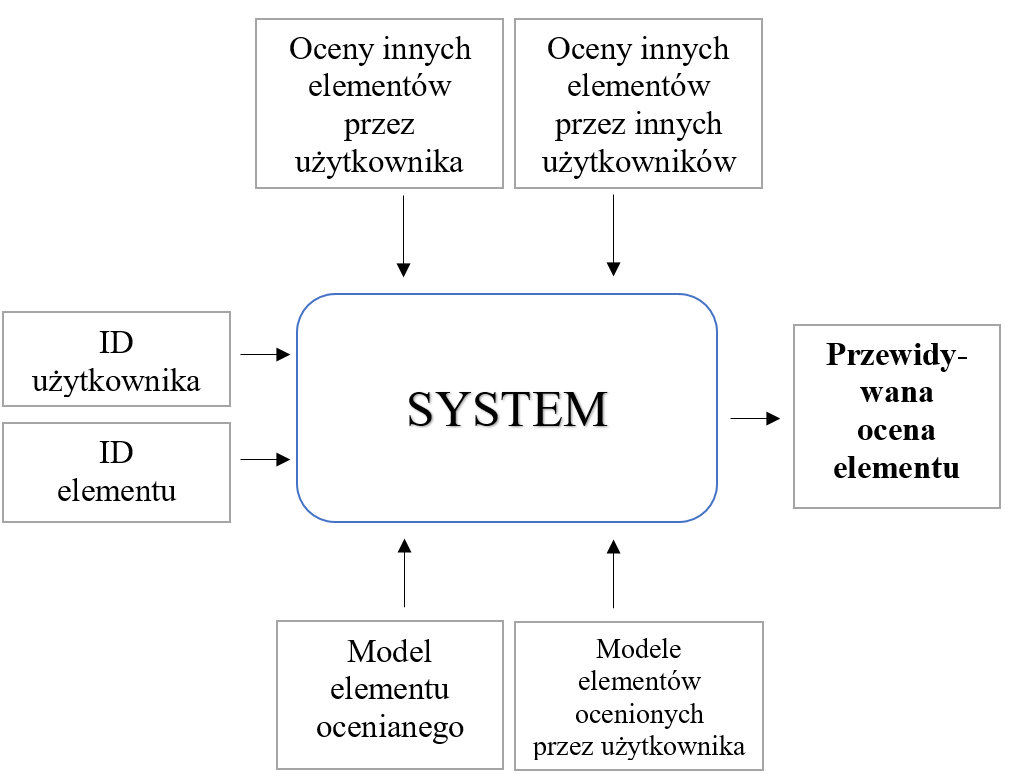
\includegraphics[width=0.7\textwidth]{blackbox}
		\caption{Model czarnoskrzynkowy}
		\label{fig:blackbox}
	\end{figure}
	
	Założeniem systemu jest uniwersalność, zatem model elementu jest uogólniony i~dostosowuje się w~zależności do domeny, w~której system jest wykorzystywany. Rys. \ref{fig:modelElementu} przedstawia reprezentację elementu w~systemie. W~zbiorze wartości mogą znaleźć się takie pozycje jak lista aktorów, reżyser (w~przypadku filmów), gatunek, wykonawca (w~przypadku muzyki), typ produktu lub cena (w~przypadku systemów typu e-commerce).
	
	\begin{figure}[!ht] 
		\centering
		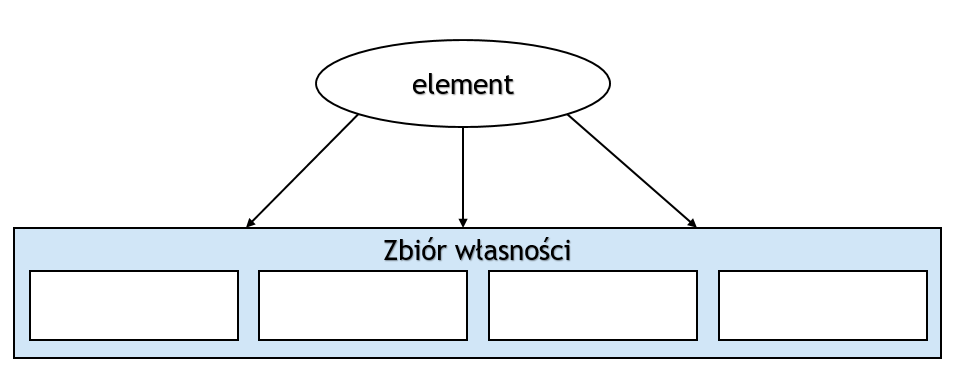
\includegraphics[width=0.7\textwidth]{modelElementu}
		\caption{Uogólniony model elementu}
		\label{fig:modelElementu}
	\end{figure}
	
	Każdy użytkownik systemu jest anonimowy. Nie jest znana jego płeć, wiek, pochodzenie itp. System nie przechowuje także informacji właściwych mediom społecznościowym, takich jak relacje między użytkownikami (przyjaźnie, śledzenie). Wiadomym jest jedynie, jakie elementy zostały ocenione i~jak zostały ocenione. Rys. \ref{fig:modelUsera} przedstawia reprezentację użytkownika w~systemie.
	
	\begin{figure}[!ht] 
		\centering
		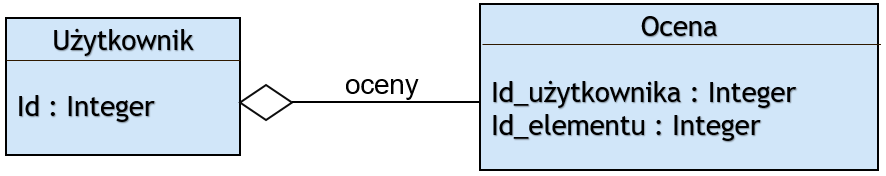
\includegraphics[width=0.7\textwidth]{modelUsera}
		\caption{Uogólniony model elementu}
		\label{fig:modelUsera}
	\end{figure}
		 
 	\section{Propozycja algorytmu filtrowania z~analizą zawartości}
	\label{s:propozycjaalgorytmucbf}
	 
	Algorytmy filtrowania z~analizą zawartości budują rekomendację na podstawie ocen, jakie zostały dotychczas wystawione przez użytkownika. Analizowane są cechy elementów i~ich wartości oraz określana jest ich siła wpływu na finalną ocenę. 
	
	W tym celu dla każdego użytkownika tworzona jest sieć neuronowa, która uczy się jego preferencji. W~projekcie wykorzystana została implementacja sieci neuronowych z~biblioteki AForge.NET Framework \cite{aforgenet}.
	 
	 \subsection{Struktura perceptronów i~funkcja aktywacji}
	 \label{sss:strukturaperceptronow}
	 
	 Wykorzystywana sieć neuronowa składa się z~trzech warstw neuronów (perceptronów). W~każdej warstwie wszystkie neurony mają konstrukcję na jak rys. \ref{fig:schematneuronu}
	 
	 \begin{figure}[!ht] 		 		 	
	 	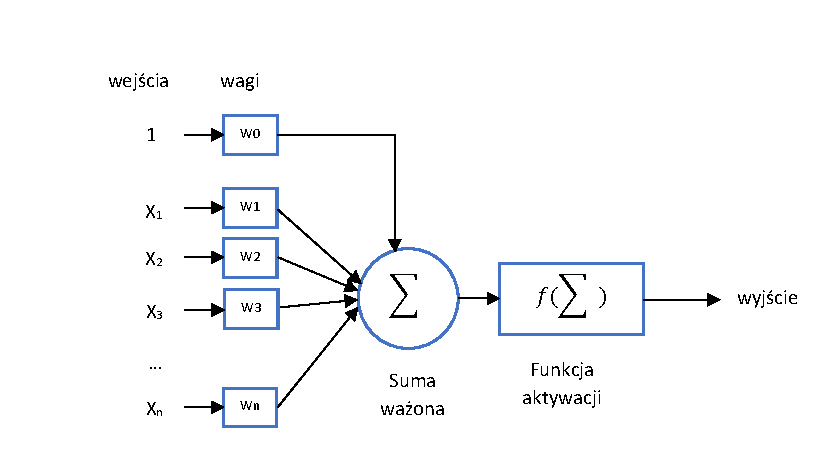
\includegraphics[width=0.9\textwidth]{schematneuron}
	 	\caption{Schemat perceptronu}
	 	\label{fig:schematneuronu}
	 \end{figure}
	 
	 Do neuronu przekazywany jest zestaw wartości w~postaci wektora $x$. Następnie obliczana jest suma ważona tych wartości w~zależności od nadanych wag $w$. Proces dobierania odpowiednich wag jest nazywany uczeniem (zob. \ref{ss:uczeniesiecineuronowej}). W~następnym kroku suma ważona przekazywana jest do funkcji aktywacji neuronu. Jeżeli funkcja przyjmie wartość wyższą lub równą niż określony próg aktywacji, to perceptron zostanie pobudzony (zwróci wartość 1). Proces ten obrazuje równanie \ref{eq:neuroneq}.
	 
	 \begin{equation}
	 \label{eq:neuroneq}
	 N(x_1, x_2, x_3, \ldots, x_n) = 
	 \begin{cases}
	 1       & \quad \text{jeśli } f(w_0 + \sum_{i=1}^{n}w_ix_i) \geq \eta\\
	 0		 & \quad \text{jeśli } f(w_0 + \sum_{i=1}^{n}w_ix_i) < \eta\\
	 \end{cases}
	 \,,
	 \end{equation}		 
	 gdzie
	 
	 \begin{conditions*}
	 	w & to wagi kolejnych wejść \\
	 	x & to wartości przekazywane do wejść \\
	 	f(u) & to funkcja aktywacji neuronu \\
	 	\eta & to próg aktywacji neuronu
	 \end{conditions*} 
	 
	 Na potrzeby algorytmu rekomendacji zdecydowano się przyjąć sigmoidalną unipolarną funkcję aktywacji neuronu (równanie \ref{eq:sigmoidal}). Funkcja przyjmuje wartości z~zakresu $[0,1]$.
	 
	 \begin{equation}
	 \label{eq:sigmoidal}
	 f(x) = \frac{1}{1 + \exp(-\alpha x)}
	 \,.
	 \end{equation}
	 Wykres funkcji wygląda jak na rys. \ref{fig:sigmoid}.
	 
	 \begin{figure}[!ht] 
	 	\centering
	 	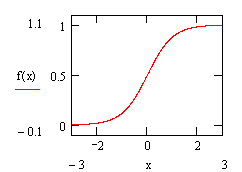
\includegraphics{sigmoid}
	 	\caption{Wykres sigmoidalnej funkcji aktywacji perceptronu \protect\cite{aforgenet}}
	 	\label{fig:sigmoid}
	 \end{figure}
	 
	 \subsection{Struktura sieci i~przebieg algorytmu}
	 \label{ss:strukturasiecineuronowej}		 
		 Pierwszym etapem algorytmu jest analiza cech elementów ocenionych przez użytkownika. Tworzona jest lista wszystkich występujących cech które powtarzają się minimum tyle razy, ile wynosi wartość  parametru \textit{minimumRepeatingFeatures}. 
		 
		 Następnie inicjowana jest sieć neuronowa. Ilość neuronów warstwy wejściowej jest równa ilości wyodrębnionych cech. Warstwa ukryta zawiera tyle neuronów ile jest to określone parametrem \textit{hiddenLayerNeurons}. Warstwa wyjściowa składa się z~tylko jednego neuronu (rys. \ref{fig:siecneuronowa}). 
		 
		 \begin{figure}%[H] %!ht 
		 	\centering
		 	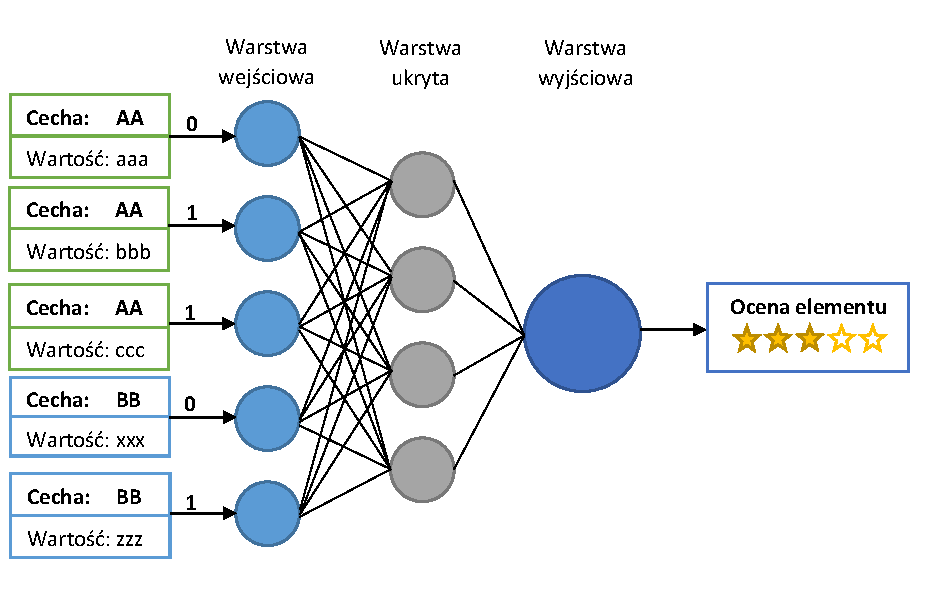
\includegraphics[width=1\textwidth]{siecneuronowa}
		 	\caption{Schemat sieci neuronowej}
		 	\label{fig:siecneuronowa}
		 \end{figure}
		 
		 W~kolejnym etapie dla każdego elementu tworzona jest mapa cech. Jeżeli element zawiera daną cechę o~danej wartości przypisywana jest wartość $1$. W~przeciwnym razie wstawiane jest $0$. Rys. \ref{fig:mapacech} przedstawia przykładową mapę cech. Tak przygotowana lista przekazywana jest do sieci neuronowej. 
		 
		 \begin{figure}%[H]  %!ht
		 	\centering
		 	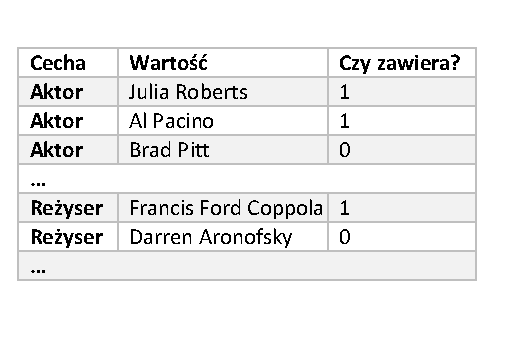
\includegraphics[width=0.7\textwidth]{mapacech}
		 	\caption{Mapa cech elementu. Wiadomo, że element X zawiera cechę ,,Aktor'' o~wartościach ,,Julia Roberts, Al Pacino'' oraz cechę ,,Reżyser'' o~wartości ,,Francis Ford Coppola''. Element nie zawiera cechy ,,Aktor'' o~wartości ,,Brad Pitt'' ani cechy ,,Reżyser'' o~wartości ,,Darren Aronofsky'' więc w~te miejsca wstawiane jest $0$.}
		 	\label{fig:mapacech}
		 \end{figure}
		 
		 Na wyjściu sieć zwraca przewidywaną ocenę elementu.
		 		 
		 
	 \subsection{Uczenie sieci neuronowej}
		 \label{ss:uczeniesiecineuronowej}
		 
		 Aby sieć zwracała jak najlepsze wyniki musi wcześniej zostać nauczona preferencji użytkownika. Uczenie sieci polega na odnalezieniu odpowiednich wag dla każdego wejścia każdego perceptronu sieci (budowa perceptronu zob. \ref{sss:strukturaperceptronow}). Proces ten można zapisać w~postaci
		 
		 \begin{equation}
		 \label{eq:weightadaptation}
		 W_{ij}(n+1) = W_{ij}(n) + \Delta W_{ij}(n) 
		 \,,
		 \end{equation}		 		 
		 gdzie
		 
		 \begin{conditions*}
		 	W_{ij}(n) & to poprzednie wagi wejść \\
		 	W_{ij}(n+1) & to nowe wagi wejść \\
		 	n & numer cyklu uczącego 
		 \end{conditions*} 
		 
		 Dostrajanie wartości wag można wykonać na wiele sposobów. Można wyróżnić uczenie nadzorowane (z~nauczycielem), uczenie z~krytykiem (ang. \textit{reinforcement learning}) i~uczenie samoorganizujące się (bez nadzoru) \cite{osowski1996sieci}.
		 
		 Na potrzeby systemu rekomendacji z~analizą zawartości opisywanego w~tej pracy wykorzystane zostały trzy metody uczenia: algorytm propagacji wstecznej, algorytm RPROP i~algorytm genetyczny (zob. \ref{sss:backprop}). Wymienione metody należą do kategorii uczenia nadzorowanego. 

	 \section{Propozycja nowych algorytmów hybrydowych}
		 
		 Zaproponowane nowe algorytmy są hybrydą filtrowania kolaboratywnego i~filtrowania z~analizą zawartości. Obie te metody uruchamiane są osobno, w~efekcie dla każdej pary użytkownik\-/element uzyskiwane są dwie  predykowane oceny z~obu metod:  $r_{content-based_{ui}}$ i~$r_{collaborative_{ui}}$. Ponadto, znany jest błąd $d \geq 0$, z~jakim zakończyło się uczenie sieci neuronowej dla użytkownika $u$. Przewidywana ocena obliczana jest wzorem:
		 
		 \begin{equation}
		 	\label{eq:hybrid}		 	
		 	 r_{ui} = (\frac{1}{k})^d \cdot r_{content-based_{ui}} + (1-(\frac{1}{k})^d) \cdot r_{collaborative_{ui}}
		 	\,,
		 \end{equation}		 
		 gdzie $k$ jest parametrem konfigurowalnym (domyślnie $k = 2$), który determinuje stopień nachylenia funkcji wykładniczej. Parametr musi spełniać warunek $k>1$. Im wyższa wartość $k$, tym większy wpływ na rezultat ma wynik algorytmu kolaboratywnego. Zależność tę obrazuje rys. \ref{fig:hybridfunction}.
		 
		 \begin{figure}[!ht] 
		 	\centering
		 	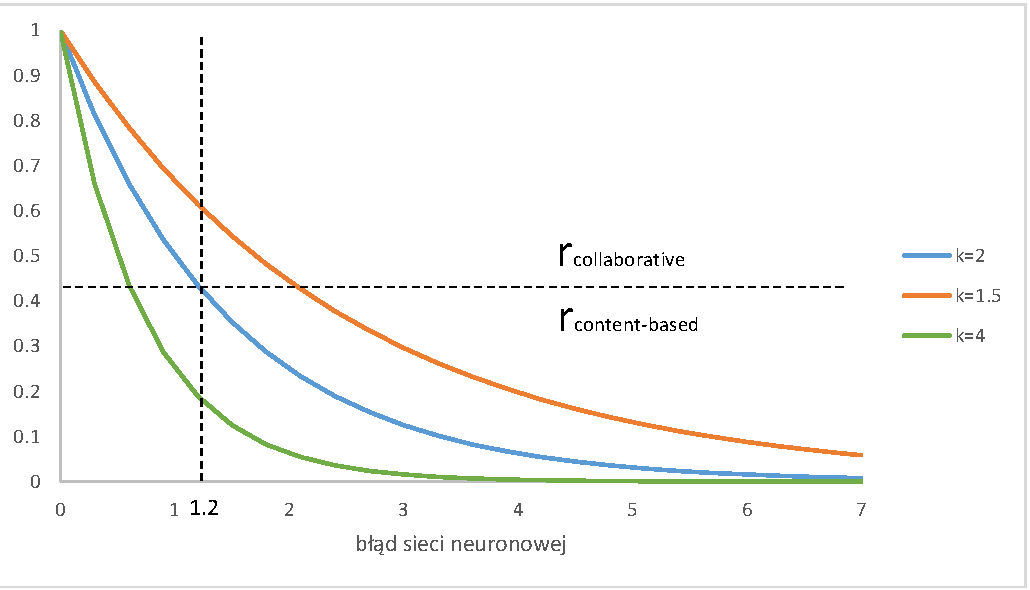
\includegraphics[width=0.7\textwidth]{hybridfunction}
		 	\caption{Wpływ parametru $k$ na wynik algorytmu. Jeżeli parametr $k=2$ a~uczenie sieci neuronowej zakończyło się z~błędem równym $d=1,2$, to końcowy stosunek wag wyniku filtrowania z~analizą zawartości do wyniku filtrowania kolaboratywnego wyniesie ok. 43,5\% do 56,5\%.}
		 	\label{fig:hybridfunction}
		 \end{figure}
		 
		 Zaimplementowanych zostało 9 algorytmów łączących różne metody filtrowania kolaboratywnego i~filtrowania z~analizą zawartości:
		 
		 \begin{enumerate}
		 	\item \textbf{Matrix Factorization i~sieć neuronowa uczona metodą propagacji wstecznej} -- ten wariant łączy ze sobą szybki, ale najmniej efektywny ze wszystkich wykorzystywanych metod kolaboratywnych algorytm z~dość dokładnym, lecz nie najszybszym sposobem uczenia sieci neuronowej. Spodziewanym efektem jest dość stosunkowo wysoki wpływ algorytmu z~analizą zawartości na końcowy wynik. 
		 	\item \textbf{Matrix Factorization i~sieć neuronowa uczona metodą RPROP} -- jako, że zarówno metoda RPROP jak i~Matrix Factorization są najszybszymi algorytmami wśród innych zaprezentowanych propozycji, to takie połączenie dostarcza najszybsze, lecz najmniej efektywne rozwiązanie.
		 	\item \textbf{Matrix Factorization i~sieć neuronowa uczona algorytmem genetycznym} -- sieć neuronowa uczona algorytmem genetycznym cechuje się dość wysoką efektywnością, jednakże czas uczenia jest dużo większy w~porównaniu do innych metod. Spodziewanym efektem jest stosunkowo wysoki wpływ algorytmu z~analizą zawartości na końcowy wynik przy dość wolnym czasie wykonania.
		 	\item \textbf{Biased Matrix Factorization i~sieć neuronowa uczona metodą propagacji wstecznej} -- algorytm Biased Matrix Factorization cechuje się wyższą skutecznością niż Matrix Factorization ale też dłuższym czasem wykonania. W~związku z~tym taki wariant będzie wolniejszy ale bardziej efektywny niż wariant nr 1.
		 	\item \textbf{Biased Matrix Factorization i~sieć neuronowa uczona metodą RPROP} -- analogicznie jak powyżej, taki wariant powinien cechować się wyższą skuteczności i~niższą prędkością niż wariant 2. Z~drugiej strony będzie on szybszy i~mniej skuteczny niż wariant 4.
		 	\item \textbf{Biased Matrix Factorization i~sieć neuronowa uczona algorytmem genetycznym} -- z~powodu wykorzystania algorytmu genetycznego będzie to jeden z~wolniejszych wariantów, ale cechować się będzie dobrą efektywnością.	 	
		 	\item \textbf{SVD++ i~sieć neuronowa uczona metodą propagacji wstecznej} -- algorytm SVD++ jest najwolniejszą metodą filtrowania kolaboratywnego ale jednocześnie najefektywniejszą. Połączenie z~siecią neuronową uczoną metodą propagacji wstecznej może dać najlepsze wyniki ze wszystkich wariantów.
		 	\item \textbf{SVD++ i~sieć neuronowa uczona metodą RPROP} -- w~tym wypadku długi czas wykonania algorytmu SVD++ może zbilansować szybki czas algorytmu RPROP. Uzyskany wynik możenie być tak dobry jak w~wariancie 7 z~powodu niższej efektywności RPROP niż klasycznej propagacji wstecznej.
		 	\item \textbf{SVD++ i~sieć neuronowa uczona algorytmem genetycznym} -- jest to najwolniejszy wariant ze wszystkich lecz może konkurować efektywnością z~wariantem 7 (zależnie od konfiguracji algorytmu genetycznego).
		 \end{enumerate}
	 
		 \subsection{Zalety zaproponowanych metod}
		 
		 Największą przewagą zaproponowanych algorytmów jest to, że łączą on zalety filtrowania z~analizą zawartości i~filtrowania kolaboratywnego minimalizując jednocześnie ich wady poprzez dynamiczne dobieranie proporcji ich wpływu na końcowy wynik. Nowa metoda cechuje się uniwersalnością, gdyż model elementu zawierający jego własności budowany jest automatycznie. Jednocześnie nie są wymagane informacje o~użytkowniku inne, niż to jakie elementy ocenił i~jak je ocenił. 
		 
		 Im więcej zostanie dostarczonych informacji na temat elementów, tym lepsze będą wyniki. Jednakże w~przypadku braku takowych informacji metoda ciągle będzie działać,  wówczas wynik będzie opierał się głównie na rezultatach filtrowania kolaboratywnego.
		 
		 Analogicznie, w~przypadku małej liczby powiązań z~innymi użytkownikami, zaproponowany algorytm hybrydowy ulepszy wynik filtrowania kolaboratywnego dzięki czynnikowi filtrowania z~analizą zawartości. 
		 
		 W~zależności od tego, czy bardziej istotna jest dokładność czy czas wykonania, można dobrać odpowiedni wariant nowej metody. 
		 
		 W~zależności od konstrukcji danych można tak dopasować parametr $k$, aby wynik był dokładniejszy. W~przypadku takiej konfiguracji danych, gdzie macierz użytkownik\-/element jest wypełniona w~małym stopniu, istnieje możliwość takiego dostrojenia parametru, żeby większy wpływ na wynik końcowy miało filtrowanie z~analizą zawartości. W~przypadku odwrotnym preferowanym jest aby większy wpływ na wynik końcowy miał algorytm filtrowania kolaboratywnego.
		 
		 \subsection{Wady zaproponowanych metod}
		 
		 Największą wadą nowej metody jest wyższa złożoność. Czas budowania modelu jest sumą czasów budowania modelu kolaboratywnego i~modelu filtrowania z~analizą zawartości. 
		 
		 Istnieje też ryzyko, że w~momencie gdy wynik filtrowania kolaboratywnego będzie bardzo zły, to rezultat osiągnięty przez nową metodę będzie gorszy niż z~samego filtrowania z~analizą zawartości. 
		 
		 Niebezpieczeństwem może też być złe dopasowanie parametru $k$ do przetwarzanych danych.
 
\chapter{Ocena eksperymentalna}
\shortTitle{Ocena eksperymentalna}
	\section{Opis metody badawczej}
	
		W celu zbadania jakości algorytmów zaprojektowany został eksperyment. W~pierwszej kolejności definiowane są wartości parametrów, zgodnie z~którymi ma zostać wykonany kod algorytmów. 
		Dla parametru podlegającemu testom definiowany jest zakres wartości. 
		
		Następnie do pamięci ładowany jest zestaw danych zawierający oceny elementów przez użytkowników oraz dodatkowe własności elementów (jeżeli testowanym algorytmem jest filtrowanie z~analizą zawartości lub filtrowanie hybrydowe). W~celu przeprowadzenia walidacji krzyżowej zbiór dzielony jest $k$ części. Z~nich konstruowanych jest następnie $k$ par: zbiór testowy-zbiór treningowy. Rozmiar każdego zbioru testowego jest równy rozmiarowi jednej części ($\frac{1}{k}$ liczby wszystkich ocen) a~rozmiar zbioru treningowego to $k-1*$rozmiar części. W~czasie przeprowadzanych eksperymentów przyjęto $k=5$.
		
		Dla każdej pary zbiorów treningowego i~testowego przeprowadzana jest nauka i~sprawdzanie algorytmu. Z~każdego przebiegu błędy są sumowane a~na końcu wyciągana jest średnia.
		
		Przebieg algorytmu wygląda następująco:
		
		\def\alghoritm6{Przebieg eksperymentu}
		\begin{breakablealgorithm}
			\caption{\alghoritm6}
			\myalgorithm{\alghoritm6}
			\label{aq:experiment}
			\begin{algorithmic}	
				\STATE $recommenderType \leftarrow$ silnik rekomendacji: filtrowanie kolaboratywne, filtrowanie z~analizą zawartości bądź filtrowanie hybrydowe 			
				\STATE $parameters[] \leftarrow $ ustaw parametry wybranego algorytmu rekomendacji
				\STATE $pt[] \leftarrow $ zdefiniuj wartości parametru testowanego				
				\STATE $cbUsersCount \leftarrow$ liczba użytkowników do pobrania do filtrowania z~analizą zawartości
				\STATE $cfUsersCount \leftarrow$ liczba użytkowników do pobrania do filtrowania kolaboratywnego
				\STATE $minimumRepeatingFeatures \leftarrow $ minimalna ilość powtórzeń danej cechy 
				\STATE $pt[] \leftarrow $ zdefiniuj wartości parametru testowanego
				\STATE $k \leftarrow $ parametr podziału dla do sprawdzianu krzyżowego 
				
				\FOR {$i \in pt $}
					\STATE $parameters[parametrZmienny]:= i$					
					\textbf{//Faza pobierania danych}			
					\IF {$recommenderType == $ filtrowanie kolaboratywne \textbf{or} filtrowanie hybrydowe}					
					\STATE $cfUsers \leftarrow$ załaduj oceny $cfUsersCount$ użytkowników;
					\ELSIF {$recommenderType == $ filtrowanie z~analizą zawartości \textbf{or} filtrowanie hybrydowe}
					\STATE $cbUsers \leftarrow$ załaduj oceny $cbUsersCount$ użytkowników wraz z~własnościami elementów;
					\ENDIF
					
					\STATE {podziel zbiory na k~części}
					
					\textbf{//Faza nauki}
					
					\FOR {$i \in k $}
					
					\STATE wybierz testowy $i$ a~z pozostałych danych utwórz zbiór treningowy
					
					\IF {$recommenderType == $ filtrowanie kolaboratywne}					
					\STATE $cfRecommender \leftarrow$ ucz filtrowaniem kolaboratywnym wykorzystując zbiór treningowy $cfUsers$;
					\ELSIF {$recommenderType == $ filtrowanie z~analizą zawartości}
					\STATE $cbRecommender \leftarrow$ ucz filtrowaniem z~analizą zawartości wykorzystując zbiór treningowy $cbUsers$;
					\ELSIF {$recommenderType == $ filtrowanie hybrydowe}
					\STATE $hybridRecommender \leftarrow$ ucz filtrowaniem hybrydowym wykorzystując zbiory treningowe $cbUsers$ i~$cfUsers$;
					\ENDIF
					
					\STATE{Wykonaj test silnika rekomendacji wykorzystując zbiór testowy}
					\STATE{Oblicz błąd RMSE i~MAE}	
					
					\ENDFOR
					
					\STATE{Oblicz średnią błędów RMSE i~MAE ze wszystkich iteracji}
					\STATE Wyświetl wyniki 
				\ENDFOR

			\end{algorithmic}
		\end{breakablealgorithm}
			
		\subsection{Miara oceny}
		
		W celu zbadania jakości algorytmów zostały zastosowane miary oceny: średnia kwadratowa błędów (RMSE) i~średni błąd bezwzględny (MAE).
		
		\subsubsection{Średnia kwadratowa błędów}
	
		Średnia kwadratowa błędów (ang. RMSE -- \textit{root mean square error}) jest często wykorzystywaną miarą służącą zmierzeniu różnicy pomiędzy wartościami przewidywanymi a~rzeczywistymi (obserwowanymi). 
		
		RMSE jest stosunkowo dobrą miarą dokładności ale tylko w~celu porównania  różnych modeli dla tego samego zestawu danych. RMSE jest zależne od skali, zatem nie sprawdza się najlepiej w~przypadku porównywania ze sobą różnych zmiennych \cite{hyndman2006another}.
		
		Średnią kwadratową błędów wylicza się ze wzoru:
		
		\begin{equation}
			\label{eq:rmse}
			RMSE = \sqrt{ \frac{1}{n} \sum_{i=1}^{n} (\hat{y}_i - y_i)^2 }
			\,,
		\end{equation}	
		gdzie
		
		\begin{conditions*}
			\hat{y}_i & to wartość przewidywana \\
			y_i  &  to wartość rzeczywista
		\end{conditions*} 
		
		Im niższa wartość RMSE tym bardziej zbliżone są wartości przewidywane do rzeczywistych, zatem tym lepszy jakościowo jest model. 
		
		\subsubsection{Średni błąd bezwzględny}
		
		Inną miarą mierzenia jakości modeli predykcyjnych jest MAE (ang. \textit{mean absolute error}). Podobnie jak RMSE miara ta jest zależna od skali, zatem najlepiej sprawdza się w~działaniu na tym samym zestawie danych \cite{hyndman2006another}. 
		
		Średni błąd bezwzględny wylicza się ze wzoru:
		
		\begin{equation}
		\label{eq:mae}
		MAE = \frac{1}{n} \sum_{t=1}^{n} |\hat{y}_t - y_t|
		\,,
		\end{equation}		
		gdzie
		
		\begin{conditions*}
			\hat{y}_i & to wartość przewidywana \\
			y_i  &  to wartość rzeczywista
		\end{conditions*} 
	
	
		\subsection{Zbiory danych}
		
		W celu uzyskania obiektywnych wyników algorytmy zostały przetestowane na dwóch różnych bazach danych z~dwóch różnych domen. Eksperyment nie ma na celu porównania wyników między różnymi zestawami danych, lecz porównanie wyników testowanych algorytmów w~różnych warunkach. 
		
		\subsubsection{MovieLens}
		MovieLens \cite{harper2016movielens} to baza zawierająca oceny filmów przez użytkowników portalu movielens.org. Baza zawiera 3,706 filmów i~1,000,209 ocen wystawionych przez 6,040 unikalnych użytkowników pomiędzy 25 kwietnia 2000 a~28 lutym 2003, średnio 166 ocen na użytkownika i~270 ocen na film. Filmy oceniane są w~skali od 1 do 5, gdzie 1 jest oceną najgorszą a~5 najlepszą. 
		
		Baza zawiera tabelę łączącą numery identyfikacyjne filmów z~bazą IMDB.com. Wykorzystując te informacje baza filmów została rozszerzona o~informacje pobrane z~IMDB.com. Ostateczny kształt bazy widoczny jest na rys. \ref{fig:movielens_schema}.
		
			\begin{figure}[!ht] 
				\centering
				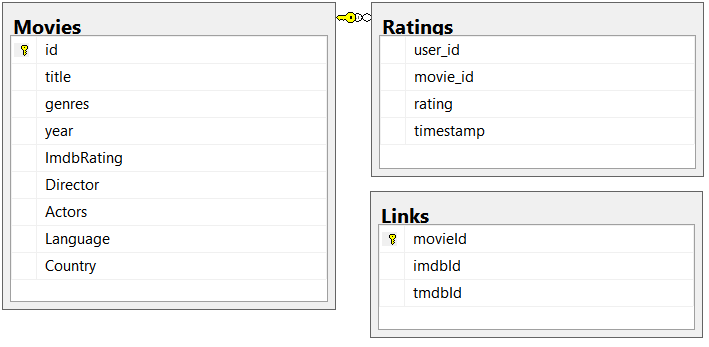
\includegraphics[width=1\textwidth]{movielens}
				\caption{Schemat bazy MovieLens}
				\label{fig:movielens_schema}
			\end{figure}
		
		\subsubsection{Amazon Meta}
		AmazonMeta to baza danych zawierająca informacje na temat zakupu produktów ze sklepu internetowego amazon.com. Dane zostały zgromadzone w~połowie roku 2006. Zawierają 548,552 produktów i~7,781,990 ocen produktów \cite{amazonmeta, leskovec2007dynamics}. Podobnie jak w~przypadku bazy MovieLens, produkty ocenione są w~skali od 1 do 5, gdzie 1 jest oceną najgorszą a~5 najlepszą. 
		
		Produkty opisane są takimi atrybutami jak nazwa, kategoria, ranking sprzedażowy, liczba produktów kupowanych jednocześnie, liczba recenzji i~średnia ocena.  
		
	\section{Środowisko symulacyjne}
	
		\subsection{Oprogramowanie}
	
		Rys. \ref{fig:program} przedstawia zrzut ekranu środowiska symulacyjnego opracowanego przez autorkę pracy na potrzeby przeprowadzenia badań algorytmów. Główny interfejs programu składa się z~trzech części: ustawienia podstawowe, okno z~wynikiem oraz panel sterujący ustawieniami zaawansowanymi. 
	
		\begin{figure}[!ht] 
			\centering
			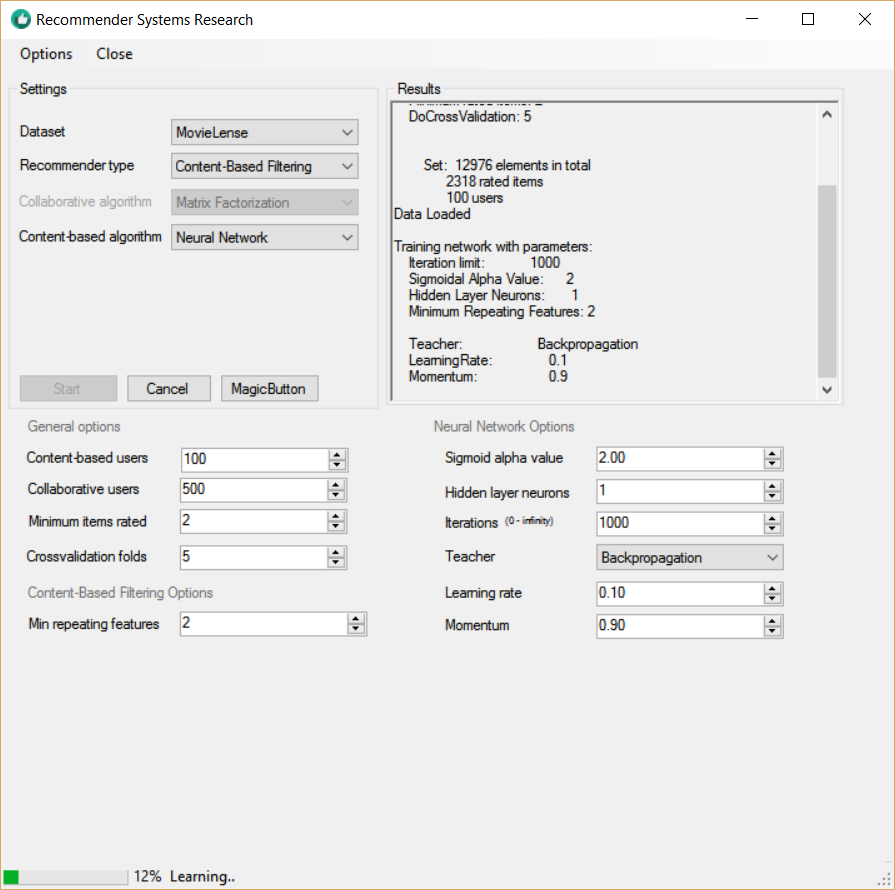
\includegraphics[width=1\textwidth]{program}
			\caption{Zrzut ekranu środowiska symulacyjnego}
			\label{fig:program}
		\end{figure}
	
		W sekcji z~ustawieniami podstawowymi możliwy jest wybór:
		\begin{itemize}
			\item bazy danych, która zostanie wykorzystana do pomiarów;
			\item typu algorytmu rekomendującego (filtrowanie z~analizą zawartości, filtrowanie kolaboratywne bądź algorytm hybrydowy)
			\item w~przypadku wyboru kolaboratywnego filtrowania lub filtrowania hybrydowego możliwy jest wybór typu algorytmu: Matrix Factorization, Biased Matrix Factorization lub SVD++.
			\item w~przypadku wyboru filtrowania z~analizą zawartości lub filtrowania hybrydowego automatycznie wybierany jest algorytm oparty na sieci neuronowej. 
		\end{itemize}
		 
		 Widok ustawień zaawansowanych zmienia się w~zależności od wybranego filtrowania. W~przypadku wyboru filtrowania z~analizą zawartości istnieje możliwość regulowania parametrów sieci neuronowej. W~każdym wariancie można regulować kryteria doboru zestawu danych.
		 
		 Kryteria doboru zestawu danych są następujące:
		 
		 \begin{itemize}
		 	\item \textbf{Liczba użytkowników CBF} (\textit{cbUsersCount}) -- liczba użytkowników uwzględnianych w~metodzie filtrowania z~analizą zawartości;
		 	\item \textbf{Liczba użytkowników CF} (\textit{cfUsersCount}) -- liczba użytkowników uwzględnianych w~metodzie filtrowania kolaboratywnego;
		 	\item \textbf{Minimum ocenionych elementów} (\textit{minimumItemsRated}) -- minimalna liczba elementów, które użytkownik ocenił aby zostać uwzględnionym w~czasie przebiegu algorytmu;
		 	\item \textbf{Minimum powtarzających się cech} (\textit{minimumRepeatingFeatures}) -- minimalna ilość powtórzeń danej cechy elementów, aby była brana pod uwagę w~trakcie budowania rekomendacji;
		 	\item \textbf{Parametr walidacji krzyżowej} (\textit{crossvalidationFolds}) -- ilość podzbiorów, na które dzielony jest główny zbiór w~trakcie walidacji krzyżowej. 
		 \end{itemize}
		 
		 Parametry sieci neuronowej podlegające strojeniu to:

		 \begin{itemize}
		 	\item \textbf{$\alpha$} -- parametr funkcji aktywacji sieci neuronowej;
		 	\item \textbf{Ilość neuronów w~warstwie ukrytej} (\textit{hiddenLayerNeurons}) -- liczba neuronów w~warstwie ukrytej;
		 	\item \textbf{Maksymalna ilość iteracji nauki} (\textit{iterationLimit}) -- maksymalna liczba iteracji uczenia sieci neuronowej;
		 	\item \textbf{Algorytm uczący} (\textit{teacherFunction}) -- algorytm uczący sieć neuronową: propagacja wsteczna, rprop (resilient backpropagation) lub algorytm genetyczny;
		 	\item \textbf{Rozmiar populacji} (\textit{populationSize}) -- w~przypadku wyboru algorytmu genetycznego -- rozmiar każdej kolejnej populacji.
		 	
		 \end{itemize}	 
		
		\subsection{Sprzęt}
		
		Wszystkie badania zostały przeprowadzone w~tych samych warunkach na komputerze klasy PC działającym pod kontrolą 64\-/bitowego systemu Windows 10 Pro. Konfiguracja sprzętowa wygląda następująco:
		
		\begin{center}
			\begin{tabular}{ r  l  }
				Procesor: & Intel Core i5\-/6200U 2.30GHz \\ 
				RAM: & 8 GB \\  
				Typ dysku twardego: & SSD     
			\end{tabular}
		\end{center}
	
	\section{Eksperymentalne dopasowanie parametrów sieci neuronowej}
	
		Pierwszy przeprowadzony eksperyment miał na celu dopasowanie optymalnych parametrów sieci neuronowej dla filtrowania z~analizą zawartości odrębnie dla baz MovieLens i~AmazonMeta.
		
		\subsection{Strojenie sieci dla bazy MovieLens}
		\label{ss:strojeniemovielens}
			\subsubsection{Dopasowanie maksymalnej liczby iteracji}
			\label{exp:expiterations}
			
				Uczenie sieci neuronowej odbywa się w~pętli tak długo, jak wartość błędu na wyjściu spadnie poniżej określonej wartości bądź przekroczona zostanie maksymalna ilość iteracji. Eksperyment miał na celu zbadanie wartości błędów w~zależności od liczby iteracji.
					
				\begin{center}
					\begin{longtable}{ | R{7cm}   m{8cm} |}
						\hline
						\multicolumn{2}{|c|}{\textbf{Konfiguracja parametrów podstawowych}} \\
						\hline
						Baza danych: & MovieLens \\
						Testowana metoda: & Filtrowanie z~analizą zawartości \\
						\hline
						\multicolumn{2}{|c|}{\textbf{Konfiguracja filtrowania z~analizą zawartości}} \\
						\hline
						Algorytm: & Sieć neuronowa uczona propagacją wsteczną, RPROP i~algorytmem genetycznym \\
						Maksymalna ilość iteracji nauki: & ? \\				
						Ilość neuronów w~warstwie ukrytej: & 1 \\
						Współczynnik bezwładności: & 0.9 \\
						Współczynnik uczenia: & 0.1 \\
						Parametr funkcji aktywacji $\alpha$: & 2.0 \\
						Rozmiar populacji: & 100 \\
						Minimum powtarzających się cech: & 10 \\
						Minimum ocenionych elementów przez użytkownika: & 10 \\
						Ilość testowanych użytkowników: & 10 \\				
						\hline
						\caption{Konfiguracja dla eksperymentu maksymalnej liczby iteracji}
					\end{longtable}
				\end{center}
				
				Wyniki eksperymentu przedstawiają wykresy \ref{fig:expiterations_rmse} i~\ref{fig:expiterations_time} oraz tabela \ref{tab:expiterations}.  
				
				\begin{longtable}[H]{r||rr|rr|rr}		
					\label{tab:expiterations}		
					\textbf{L. iter.} & \multicolumn{2}{c|}{\textbf{Propagacja wsteczna}}  & \multicolumn{2}{c|}{\textbf{RPROP}} & \multicolumn{2}{c}{\textbf{Algorytm genetyczny}}  \\
					\hline
					& \textbf{RMSE} & \textbf{czas} & \textbf{RMSE} & \textbf{czas} & \textbf{RMSE} & \textbf{czas} \\
					\hline
					100 & 1.03402 & 155 & 1.081065 & 139 & 1.042103 & 2824 \\
					1000  & 1.022469 & 564 & 1.055915 & 463 & 1.033005 & 24831  \\
					3000  & 1.035766 & 1770 & 1.054472 & 1581  & 1.038922 & 70579  \\
					10000 & 1.058892  & 5444 & 1.081511  & 4567  & 1.068489 & 239775 \\
					\caption{Zależność błędu algorytmu wyrażonego za pomocą RMSE i~czasu wykonania od maksymalnej liczy iteracji (baza MovieLens).}
				\end{longtable}
				
				\begin{figure}[!ht]
					\centering
					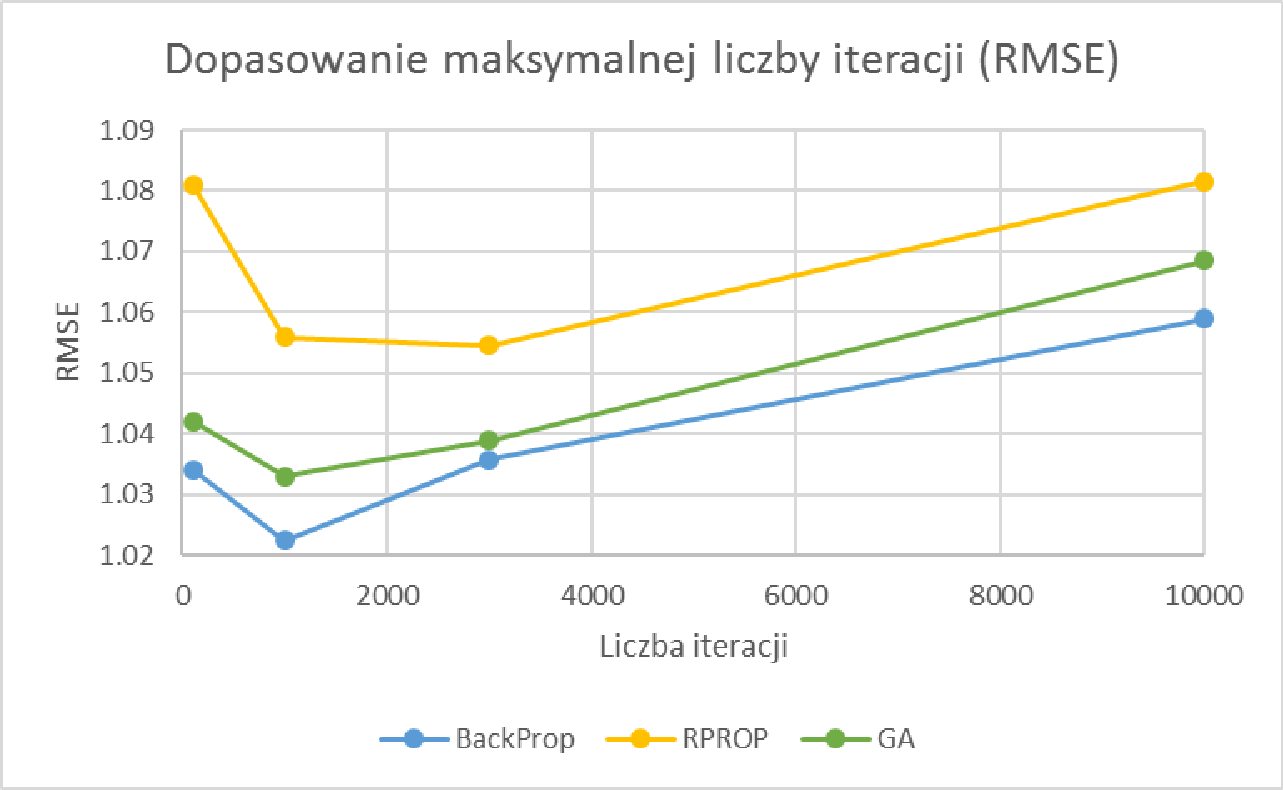
\includegraphics[width=0.7\textwidth]{expiterations_rmse}			
					\caption{Wyniki eksperymentu testującego parametr maksymalnej liczby iteracji na bazie MovieLens. Wykres przedstawia zależność pomiędzy liczbą iteracji a~błędem algorytmu wyrażonym za pomocą RMSE. Wraz ze wzrostem liczby iteracji wartość błędu maleje, jednakże po przekroczeniu pewnej wartości następuje ponowny wzrost. Wynika to z~występowania zjawiska nadmiernego dopasowania (ang. \textit{overfitting}). }
					\label{fig:expiterations_rmse}
				\end{figure}
			
				\begin{figure}[!ht]
					\centering
					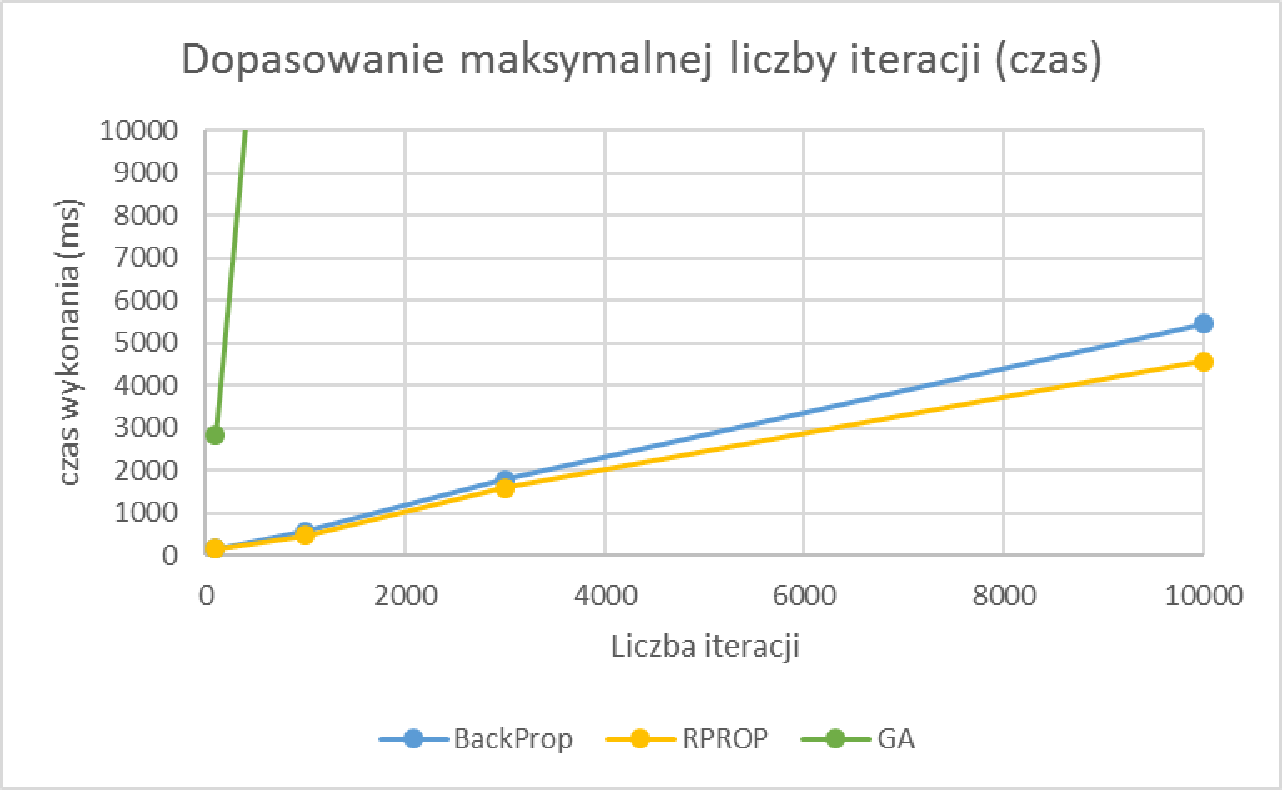
\includegraphics[width=0.7\textwidth]{expiterations_time}			
					\caption{Wyniki eksperymentu testującego parametr maksymalnej liczby iteracji na bazie MovieLens. Wykres przedstawia zależność pomiędzy liczbą iteracji a~czasem wykonania. Zgodnie z~oczekiwaniami, czas wykonania jest wprost proporcjonalny do liczby iteracji. W~trakcie tego eksperymentu potwierdzone zostały również przypuszczenia dotyczące prędkości działania algorytmów. Najszybszy okazał się RPROP, jednakże kosztem nieco większych błędów. Najgorzej wypadł algorytm genetyczny, który charakteryzował się bardzo szybko rosnącym czasem wykonania przy jednoczesnym nie najlepszym wynikiem RMSE. }
					\label{fig:expiterations_time}
				\end{figure}
					
			\subsubsection{Dopasowanie współczynnika bezwładności} 
			\label{exp:momentum}
				
			Współczynnik bezwładności jest dodatkowym współczynnikiem mającym na celu ulepszenie działania algorytmu propagacji wstecznej (zob. \ref{sss:metoda_momentum}). Eksperyment miał na celu zbadanie dla jakich wartości osiągany jest najniższy błąd.
			
			Wyniki eksperymentu przedstawia wykres \ref{fig:expmomentum} i~tabela \ref{tab:expmomentum}. 
				
			\begin{center}
				\begin{longtable}[H]{ | R{7cm}   m{8cm} |}
					\hline
					\multicolumn{2}{|c|}{\textbf{Konfiguracja parametrów podstawowych}} \\
					\hline
					Baza danych: & MovieLens \\
					Testowana metoda: & Filtrowanie z~analizą zawartości \\
					\hline
					\multicolumn{2}{|c|}{\textbf{Konfiguracja filtrowania z~analizą zawartości}} \\
					\hline
					Algorytm: & Sieć neuronowa uczona propagacją wsteczną \\
					Maksymalna ilość iteracji nauki: & 1000 \\				
					Ilość neuronów w~warstwie ukrytej: & 2 \\
					Współczynnik bezwładności: & ? \\
					Współczynnik uczenia: & 0.1 \\
					Parametr funkcji aktywacji $\alpha$: & 2.0 \\
					Minimum powtarzających się cech: & 10 \\
					Minimum ocenionych elementów przez użytkownika: & 100 \\
					Ilość testowanych użytkowników: & 5 \\				
					\hline
					\caption{Konfiguracja dla eksperymentu dopasowania wartości współczynnika bezwładności}
				\end{longtable}
			\end{center}
				
			\begin{figure}[H]
				\centering
				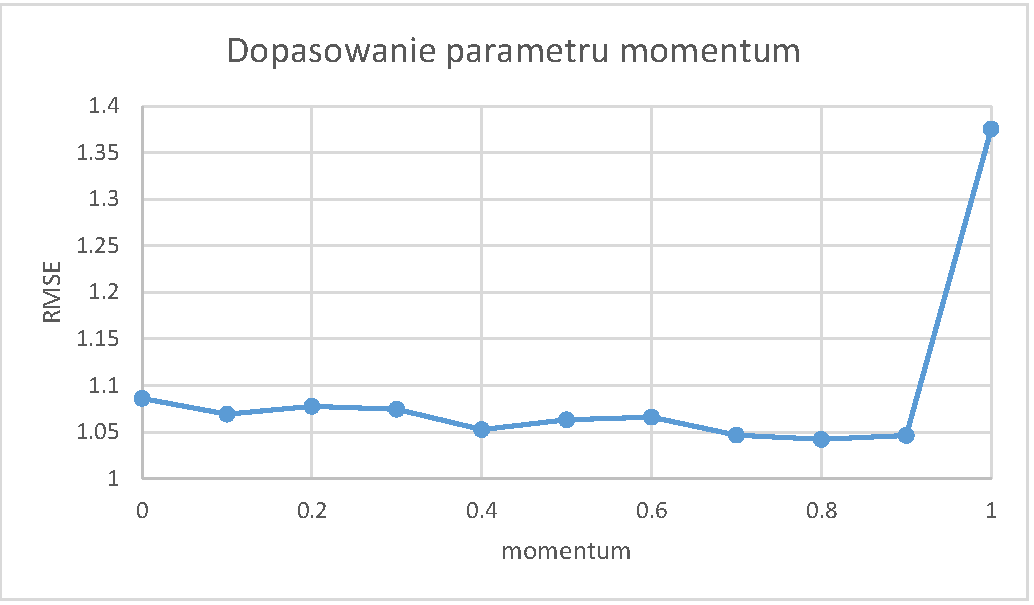
\includegraphics[width=0.7\textwidth]{expmomentum}			
				\caption{Wyniki eksperymentu testującego optymalną wartość współczynnika bezwładności na bazie MovieLens. Wykres przedstawia zależność pomiędzy wartością parametru a~błędem RMSE. W~zakresie wartości $[0,0.9]$ błąd oscyluje w~granicach podobnych wartości z~nieznaczną tendencją malejącą. Wyraźny skok na niekorzyść odnotowany jest dopiero przy momentum$=1$.}
				\label{fig:expmomentum}
			\end{figure}
					
			\begin{longtable}{r||rr}
				\label{tab:expmomentum}
				\textbf{Momentum} & \textbf{RMSE} & \textbf{MAE} \\
				\hline
				0        & 1.086007 & 0.855964 \\
				0.1      & 1.069125 & 0.851345 \\
				0.2      & 1.077596 & 0.860146 \\
				0.3      & 1.074588 & 0.851467 \\
				0.4      & 1.052529 & 0.8424   \\
				0.5      & 1.063205 & 0.846198 \\
				0.6      & 1.065994 & 0.856964 \\
				0.7      & 1.046752 & 0.83462  \\
				0.8      & 1.042235 & 0.842353 \\
				0.9      & 1.046243 & 0.840319 \\
				1        & 1.375336 & 1.071652 \\
				\caption{Zależność błędu algorytmu RMSE od wartości współczynnika bezwładności (baza MovieLens).}
			\end{longtable}
						
			\subsubsection{Dopasowanie rozmiaru populacji}
		
			Parametr rozmiaru populacji determinuje ilość osobników, jaka zostanie wygenerowana w~każdej epoce przebiegu algorytmu genetycznego (zob. \ref{ss:algorytm_genetyczny}). Eksperyment miał na celu zbadanie korelacji pomiędzy rozmiarem populacji a~błędem algorytmu rekomendacji. Mierzony jest również czas uczenia sieci neuronowej.
			
			\begin{center}
				\begin{longtable}{ | R{7cm}   m{8cm} |}
					\hline
					\multicolumn{2}{|c|}{\textbf{Konfiguracja parametrów podstawowych}} \\
					\hline
					Baza danych: & MovieLens \\
					Testowana metoda: & Filtrowanie z~analizą zawartości \\
					\hline
					\multicolumn{2}{|c|}{\textbf{Konfiguracja filtrowania z~analizą zawartości}} \\
					\hline
					Algorytm: & Sieć neuronowa uczona algorytmem genetycznym \\
					Maksymalna ilość iteracji nauki: & 1000 \\				
					Ilość neuronów w~warstwie ukrytej: & 1 \\
					Współczynnik bezwładności: & 0.9 \\
					Współczynnik uczenia: & 0.1 \\
					Parametr funkcji aktywacji $\alpha$: & 2.0 \\
					Rozmiar populacji: & ? \\
					Minimum powtarzających się cech: & 10 \\
					Minimum ocenionych elementów przez użytkownika: & 10 \\
					Ilość testowanych użytkowników: & 10 \\				
					\hline
					\caption{Konfiguracja dla eksperymentu dopasowania wielkości populacji}
				\end{longtable}
			\end{center}
			
			Wyniki eksperymentu przedstawia wykres \ref{fig:exppopulation} i~tabela \ref{tab:exppopulation}. 
			
			\begin{figure}[!ht]
				\centering
				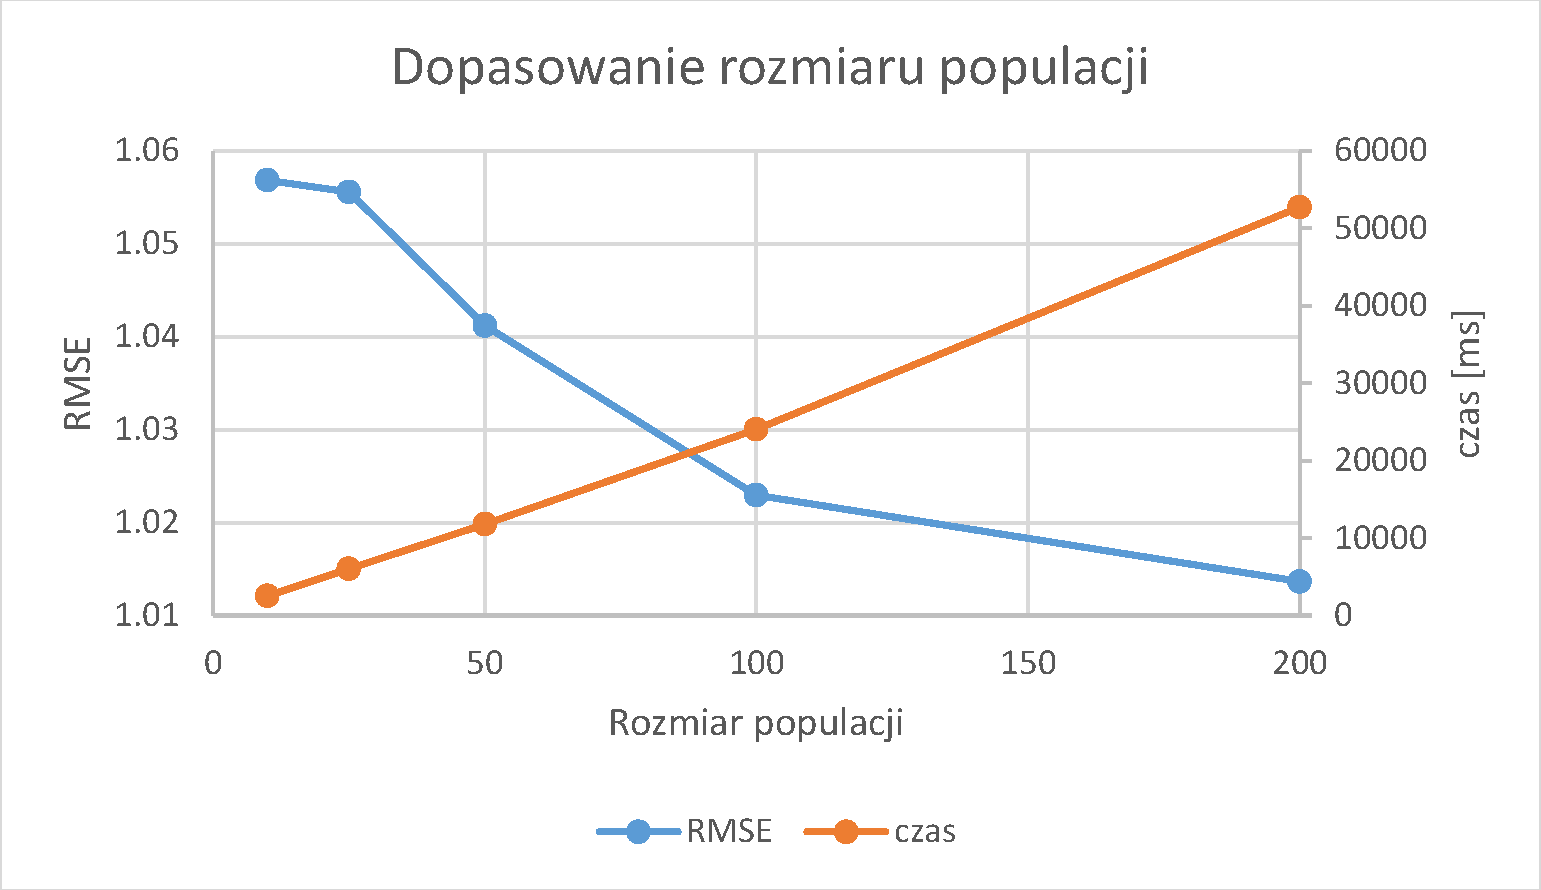
\includegraphics[width=0.7\textwidth]{exppopulation}
				\caption{Wyniki eksperymentu testującego optymalny rozmiar populacji na bazie MovieLens. Wykres przedstawia zależność pomiędzy rozmiarem a~błędem RMSE. 
				Zgodnie z~oczekiwaniami występuje dodatnia korelacja pomiędzy rozmiarem populacji a~czasem wykonania i~ujemna pomiędzy rozmiarem populacji a~błędem algorytmu rekomendacji. 
				Zależność pomiędzy rozmiarem populacji a~czasem wykonania  jest liniowa, natomiast błąd maleje wykładniczo gdy populacja osiąga większe rozmiary. Optymalnym zatem jest przyjęcie rozmiaru populacji równej $100$.}
				\label{fig:exppopulation}
			\end{figure}
			
			\begin{longtable}{r||rrr}
				\label{tab:exppopulation}
				\centering
				\textbf{Populacja} & \textbf{RMSE} & \textbf{czas} \\
				\hline
				10        & 0.861325 & 2519     \\
				25        & 0.859391 & 6015     \\
				50        & 0.850866 & 11804    \\
				100       & 0.825477 & 24062	\\
				200       & 0.816789 & 52751    \\
				\caption{Zależność błędu algorytmu RMSE od rozmiaru populacji (baza MovieLens).}
			\end{longtable}
			
			\subsubsection{Dopasowanie ilości neuronów w~warstwie ukrytej}
			
			Eksperyment miał na celu zbadanie dla jakiej liczby neuronów w~warstwie pośredniej algorytm osiąga optymalne rezultaty (zob. \ref{ss:strukturasiecineuronowej}). Wyniki eksperymentu przedstawia wykres \ref{fig:exphiddenneural} i~tabela \ref{tab:exphiddenneural}. 
		
			\begin{center}
				\begin{longtable}{ | R{7cm}   m{8cm} |}
					\hline
					\multicolumn{2}{|c|}{\textbf{Konfiguracja parametrów podstawowych}} \\
					\hline
					Baza danych: & MovieLens \\
					Testowana metoda: & Filtrowanie z~analizą zawartości \\
					\hline
					\multicolumn{2}{|c|}{\textbf{Konfiguracja filtrowania z~analizą zawartości}} \\
					\hline
					Algorytm: & Sieć neuronowa uczona propagacją wsteczną, RPROP i~algorytmem genetycznym \\
					Maksymalna ilość iteracji nauki: & 1000 \\				
					Ilość neuronów w~warstwie ukrytej: & ? \\
					Współczynnik bezwładności: & 0.9 \\
					Współczynnik uczenia: & 0.1 \\
					Parametr funkcji aktywacji $\alpha$: & 2.0 \\
					Minimum powtarzających się cech: & 10 \\
					Minimum ocenionych elementów przez użytkownika: & 10 \\
					Ilość testowanych użytkowników: & 20 \\				
					\hline
					\caption{Konfiguracja dla eksperymentu dopasowania rozmiaru ukrytej warstwy neuronów}
				\end{longtable}
			\end{center}
			
			\begin{figure}[H]
				\centering
				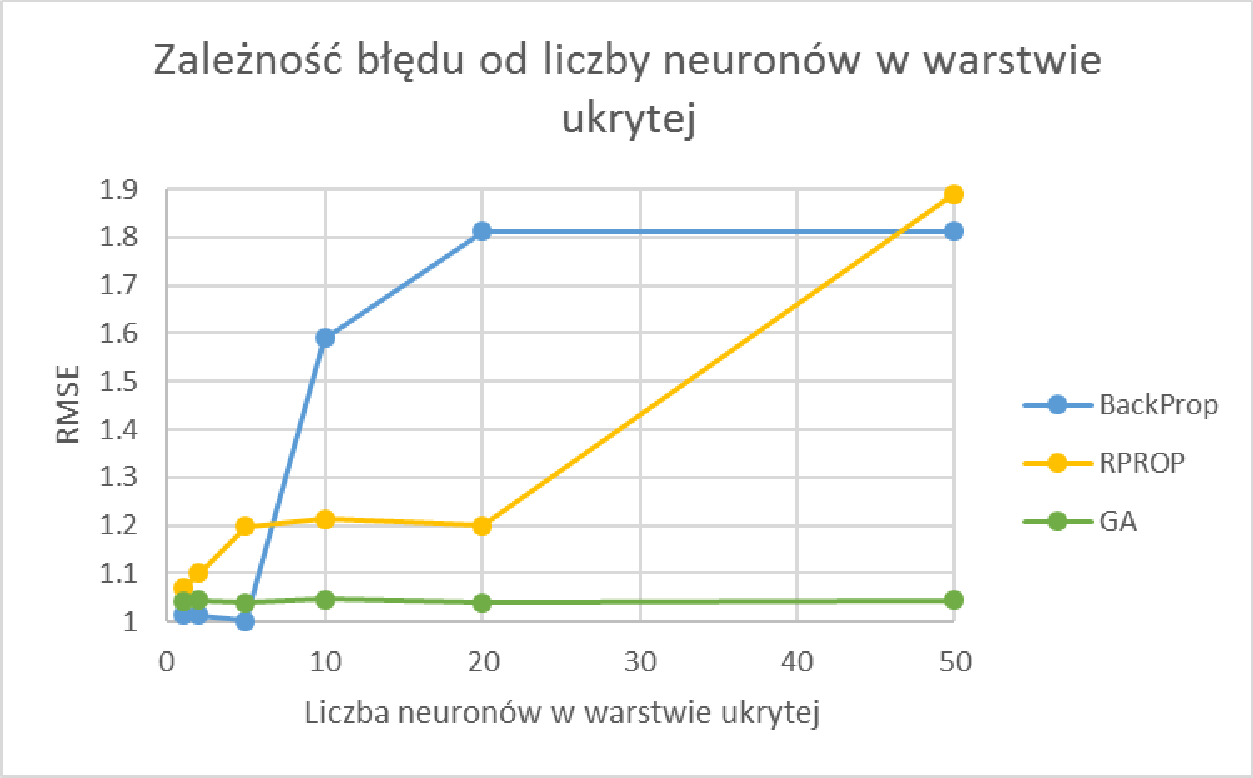
\includegraphics[width=0.7\textwidth]{exphiddenneural}
				\caption{Wyniki eksperymentu testującego optymalny rozmiar ukrytej warstwy neuronów na bazie MovieLens. Wykres przedstawia zależność pomiędzy ilością neuronów a~błędem RMSE. Wyniki prezentują się odmiennie w~zależności od typu algorytmu wykorzystanego do uczenia sieci. W~przypadku algorytmów propagacji wstecznej i~RPROP występuje dodatnia korelacja pomiędzy rozmiarem warstwy ukrytej a~błędem algorytmu rekomendacji. Dla algorytmu RPROP optymalny rezultat osiągnięty został dla zaledwie jednego neuronu w~warstwie ukrytej, dla algorytmu BackProp dla pięciu neuronów. W~tym ostatnim przypadku poprawa jest nieznaczna oscylująca w~granicach 0,01. W~przypadku algorytmu genetycznego, niezależnie od ilości neuronów wynik oscyluje na podobnym poziomie w~zakresie testowanych wartości.}
				\label{fig:exphiddenneural}
			\end{figure}
			
			\begin{longtable}{r||rr|rr|rr}
				\label{tab:exphiddenneural}
				\centering
				\textbf{L. neuronów} &  \multicolumn{2}{c|}{\textbf{Propagacja wsteczna}}  & \multicolumn{2}{c|}{\textbf{RPROP}} & \multicolumn{2}{c}{\textbf{Alg. genetyczny}}  \\
				\hline
				& \textbf{RMSE} & \textbf{MAE} & \textbf{RMSE} & \textbf{MAE} & \textbf{RMSE} & \textbf{MAE} \\
				\hline
				1                                   & 1.013503                          & 0.811766 & 1.068271 & 0.846588 & 1.042597 & 0.836481 \\
				2                                   & 1.013808                          & 0.816021 & 1.100579 & 0.862516 & 1.045096 & 0.836361 \\
				5                                   & 1.002053                          & 0.807083 & 1.197693 & 0.93349  & 1.038662 & 0.831887 \\
				10                                  & 1.589821                          & 1.232048 & 1.213635 & 0.9478   & 1.046554 & 0.835417 \\
				20                                  & 1.812912                          & 1.458733 & 1.199205 & 0.931307 & 1.039479 & 0.833191 \\
				50                                  & 1.812912                          & 1.458733 & 1.891729 & 1.562207 & 1.044693 & 0.837189\\		
				\caption{Zależność błędu algorytmu RMSE od rozmiaru ukrytej warstwy neuronowej (baza MovieLens).}
			\end{longtable}
		
			\subsubsection{Podsumowanie}
	
			Bazując na przeprowadzonych eksperymentach zostały zdefiniowane optymalne parametry algorytmu filtrowania z~analizą zawartości. Zostały one przedstawione w~tabeli \ref{tab:optimummovielens}.
		
			\begin{center}
				\begin{longtable}{ | R{7cm}   m{8cm} |}
					\hline				
					\multicolumn{2}{|c|}{\textbf{Optymalna konfiguracja filtrowania z~analizą zawartości dla bazy MovieLens}} \\
					\hline
					Maksymalna ilość iteracji nauki: & 1000 \\				
					Współczynnik bezwładności: & 0.9 \\
					Rozmiar populacji: & 100 \\
					Ilość neuronów w~warstwie ukrytej: & 1 \\
					Współczynnik uczenia: & 0.1 \\
					Parametr funkcji aktywacji $\alpha$: & 2.0 \\						
					\hline
					\caption{Konfiguracja dla eksperymentu dopasowania rozmiaru ukrytej warstwy neuronów (baza MovieLens).}
					\label{tab:optimummovielens}
				\end{longtable}
			\end{center}
		
		\subsection{Strojenie sieci dla bazy AmazonMeta}
		\label{ss:strojenieamazonmeta}
		
			W analogiczny sposób zostały przeprowadzone badania dla bazy AmazonMeta. Konfiguracja wstępna wszystkich eksperymentów była taka sama jak dla bazy MovieLens (zob. \ref{ss:strojeniemovielens}).
		
			\subsubsection{Dopasowanie maksymalnej liczby iteracji}
			
			Eksperyment miał na celu zbadanie wartości błędów w~zależności od liczby iteracji. Wyniki eksperymentu przedstawiają wykresy \ref{fig:am_expiterations_rmse} i~\ref{fig:am_expiterations_time} oraz tabela \ref{tab:am_expiterations}.  
			
			\begin{figure}[!ht]
				\centering
				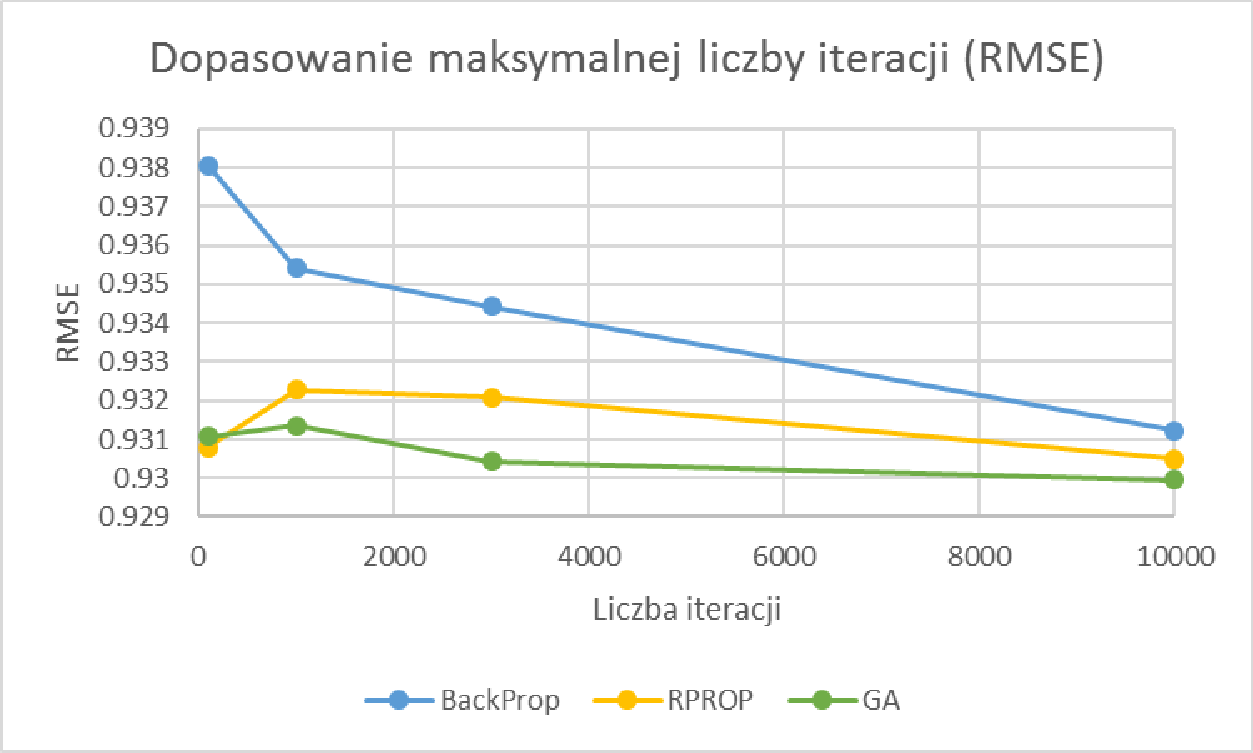
\includegraphics[width=0.7\textwidth]{am_expiterations_rmse}		
				\caption{Wyniki eksperymentu testującego parametr maksymalnej liczby iteracji na bazie AmazonMeta. Wykres przedstawia zależność pomiędzy liczbą iteracji a~błędem algorytmu wyrażonym za pomocą RMSE. Początkowo wartość błędu szybko maleje, jednakże wraz ze wzrostem liczby iteracji kąty nachylenia kolejnych odcinków krzywej ulegają zwiększeniu. Biorąc pod uwagę rosnący liniowo czas wykonania (zob. \ref{fig:am_expiterations_time}) w~pewnym momencie koszt w~postaci czasu wykonania przewyższa korzyść wynikającą z~niższego błędu RMSE. W~zakresach liczby iteracji od 100 do 2000 występują nieznaczne zachwiania, które znajdują się w~zakresie błędu statystycznego. }
				\label{fig:am_expiterations_rmse}
			\end{figure}
			
			\begin{figure}[!ht]
				\centering
				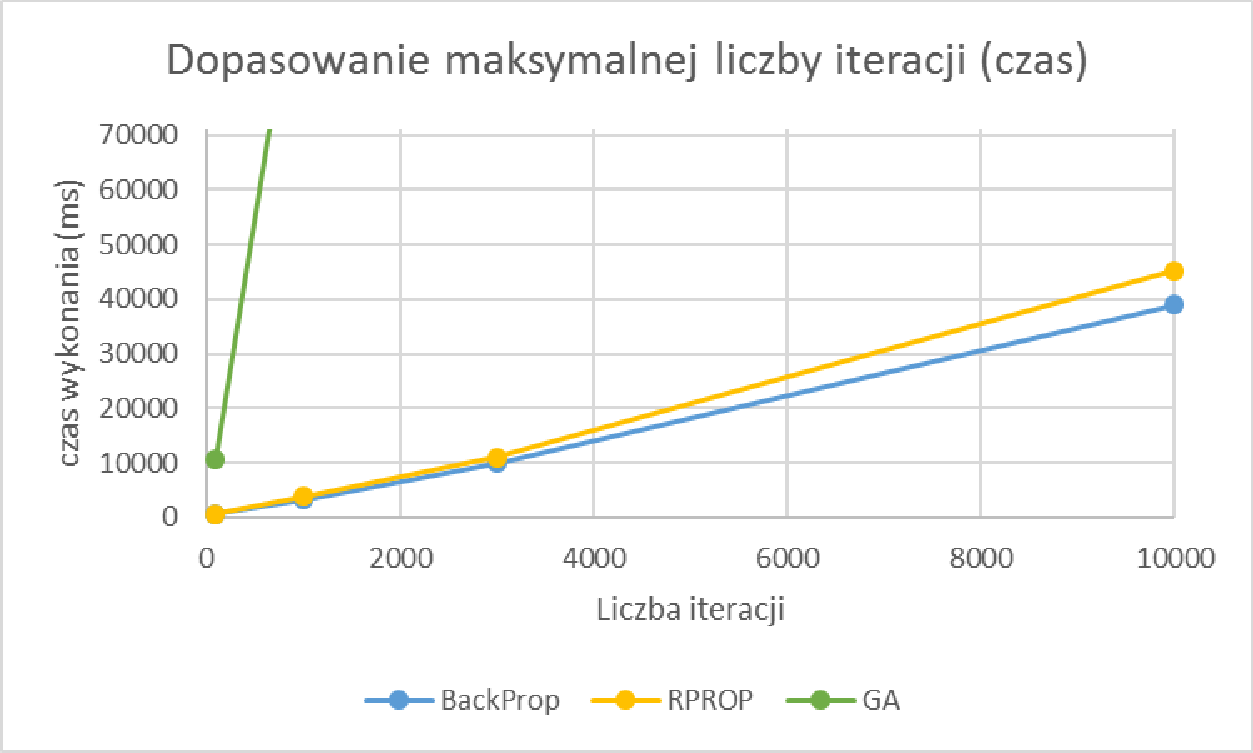
\includegraphics[width=0.7\textwidth]{am_expiterations_time}			
				\caption{Wyniki eksperymentu testującego parametr maksymalnej liczby iteracji na bazie AmazonMeta. Wykres przedstawia zależność pomiędzy liczbą iteracji a~czasem wykonania. Czas wykonania jest wprost proporcjonalny do liczby iteracji. }
				\label{fig:am_expiterations_time}
			\end{figure}
		
			\begin{longtable}[H]{r||rr|rr|rr}		
				\label{tab:am_expiterations}		
				\textbf{L. iter.} & \multicolumn{2}{c|}{\textbf{Propagacja wsteczna}}  & \multicolumn{2}{c|}{\textbf{RPROP}} & \multicolumn{2}{c}{\textbf{Algorytm genetyczny}}  \\
				\hline
				& \textbf{RMSE} & \textbf{czas} & \textbf{RMSE} & \textbf{czas} & \textbf{RMSE} & \textbf{czas} \\
				\hline
				100   & 0.938058 & 564   & 0.930788 & 585   & 0.931064 & 10641   \\
				1000  & 0.935423 & 3289  & 0.93228  & 3784  & 0.931359 & 108559  \\
				3000  & 0.934419 & 9915  & 0.932073 & 11052 & 0.930428 & 719324  \\
				10000 & 0.931222 & 38917 & 0.93049  & 45258 & 0.929965 & 3229148 \\
				\caption{Zależność błędu algorytmu wyrażonego za pomocą RMSE i~czasu wykonania od maksymalnej liczy iteracji (baza AmazonMeta).}
			\end{longtable}
			
			\subsubsection{Dopasowanie współczynnika bezwładności} 
			
			Eksperyment miał na celu zbadanie dla jakich wartości współczynnika bezwładności osiągany jest najniższy błąd. Wyniki eksperymentu przedstawia wykres \ref{fig:am_expmomentum} i~tabela \ref{tab:am_expmomentum}. 
			
			\begin{figure}[H]
				\centering
				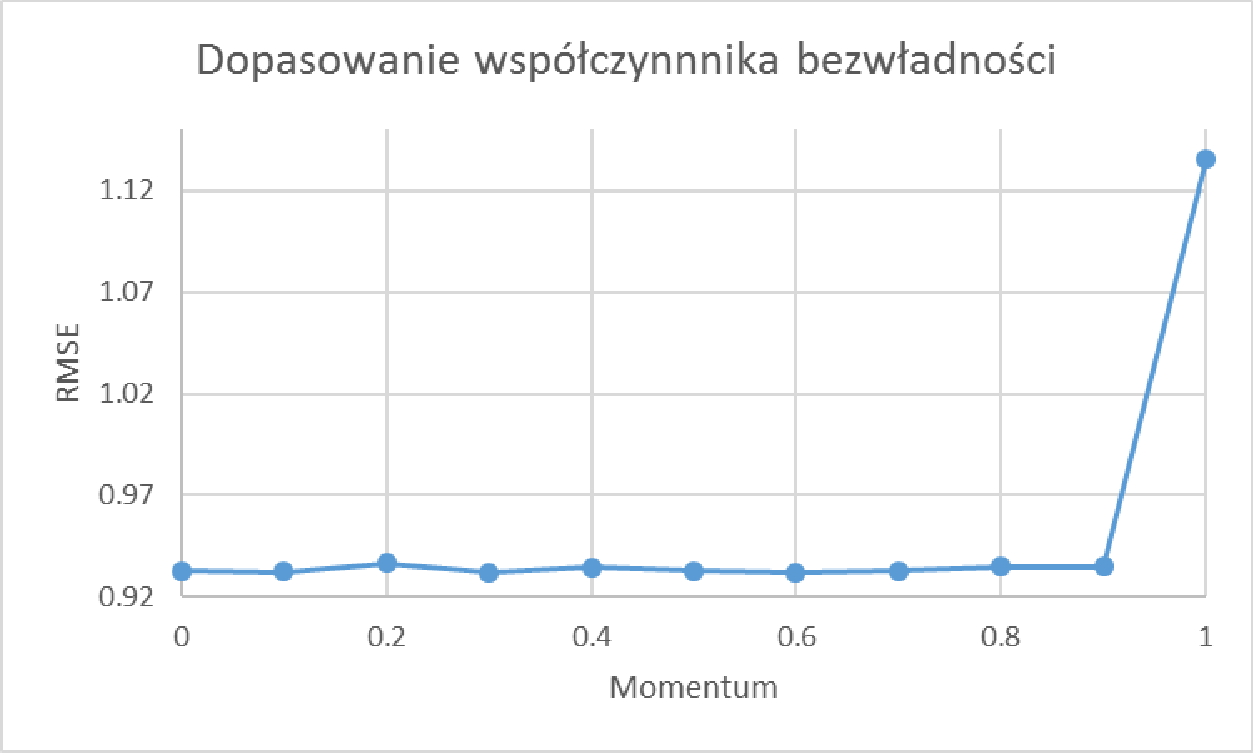
\includegraphics[width=0.7\textwidth]{am_expmomentum}			
				\caption{Wyniki eksperymentu testującego optymalną wartość współczynnika bezwładności na bazie AmazonMeta. Wykres przedstawia zależność pomiędzy wartością parametru a~błędem RMSE. W~zakresie wartości $[0,0.9]$ błąd oscyluje w~granicach podobnych wartości z~nieznaczną tendencją malejącą. Wyraźny skok na niekorzyść odnotowany jest dopiero przy momentum$=1$.}
				\label{fig:am_expmomentum}
			\end{figure}
			
			\begin{longtable}{r||rr}
				\label{tab:am_expmomentum}
				\textbf{Momentum} & \textbf{RMSE} & \textbf{MAE} \\
				\hline
				0   & 0.932621 & 0.712677 \\
				0.1 & 0.932369 & 0.711739 \\
				0.2 & 0.9366   & 0.71353  \\
				0.3 & 0.931794 & 0.718193 \\
				0.4 & 0.934477 & 0.716904 \\
				0.5 & 0.932799 & 0.717865 \\
				0.6 & 0.932026 & 0.709617 \\
				0.7 & 0.93268  & 0.714115 \\
				0.8 & 0.934683 & 0.714445 \\
				0.9 & 0.934906 & 0.716833 \\
				1   & 1.135473 & 0.8761   \\
				\caption{Zależność błędu algorytmu RMSE od wartości współczynnika bezwładności (baza AmazonMeta).}
			\end{longtable}
			
			\subsubsection{Dopasowanie rozmiaru populacji}
			
			 Eksperyment miał na celu zbadanie korelacji pomiędzy rozmiarem populacji a~błędem algorytmu rekomendacji. Wyniki eksperymentu przedstawia wykres \ref{fig:am_exppopulation} i~tabela \ref{tab:am_exppopulation}. 
			 
			 \begin{figure}[!ht]
			 	\centering
			 	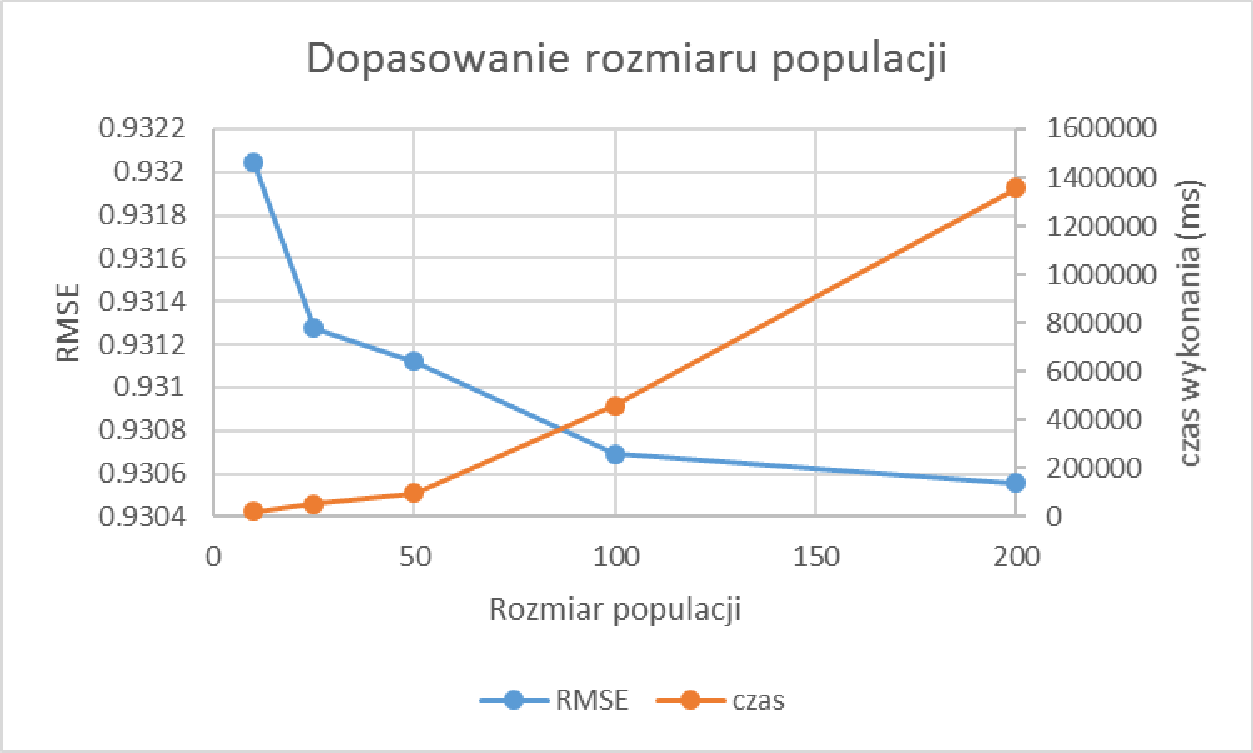
\includegraphics[width=0.7\textwidth]{am_exppopulation}
			 	\caption{Wyniki eksperymentu testującego optymalny rozmiar populacji na bazie AmazonMeta. Wykres przedstawia zależność pomiędzy rozmiarem a~błędem RMSE. 
		 		Zgodnie z~oczekiwaniami występuje dodatnia korelacja pomiędzy rozmiarem populacji a~czasem wykonania i~ujemna pomiędzy rozmiarem populacji a~błędem algorytmu rekomendacji. 
		 		Zależność pomiędzy rozmiarem populacji a~czasem wykonania  jest liniowa, natomiast błąd maleje wykładniczo gdy populacja osiąga większe rozmiary. Optymalnym zatem jest przyjęcie rozmiaru populacji równej $50$ tak, aby czas wykonania nie przekraczał 200000ms.}
			 	\label{fig:am_exppopulation}
			 \end{figure}
			
			\begin{longtable}{r||rrr}
				\label{tab:am_exppopulation}
				\centering
				\textbf{Populacja} & \textbf{RMSE} & \textbf{czas} \\
				\hline
				10        & 0.9320416  & 21277 \\
				25        & 0.9312775  & 52429 \\
				50        & 0.9311208  & 97631 \\
				100       & 0.9306905  & 460344 \\
				200       & 0.9305578  & 1356036 \\
				\caption{Zależność błędu algorytmu RMSE od rozmiaru populacji (baza AmazonMeta).}
			\end{longtable}
			
			\subsubsection{Dopasowanie ilości neuronów w~warstwie ukrytej}
			
				Eksperyment miał na celu zbadanie dla jakiej liczby neuronów w~warstwie pośredniej algorytm osiąga optymalne rezultaty. Wyniki eksperymentu przedstawiają wykresy \ref{fig:am_exphiddenneural_rmse} i~\ref{fig:am_exphiddenneural_time} oraz tabela \ref{tab:am_exphiddenneural}. 
			
				\begin{figure}[H]
					\centering
					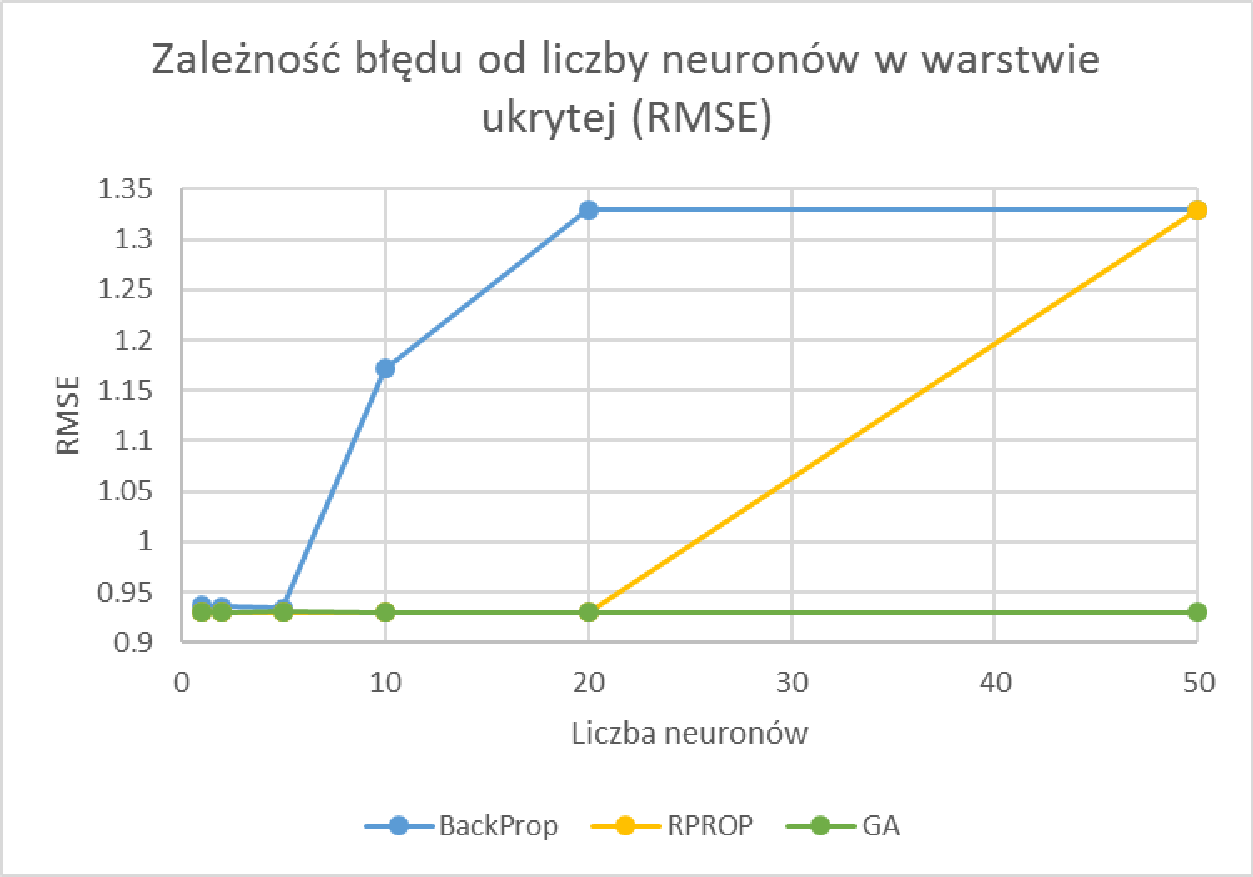
\includegraphics[width=0.7\textwidth]{am_exphiddenneural_rmse}
					\caption{Wyniki eksperymentu testującego optymalny rozmiar ukrytej warstwy neuronów na bazie AmazonMeta. Wykres przedstawia zależność pomiędzy ilością neuronów a~błędem RMSE. W~przypadku algorytmów propagacji wstecznej i~RPROP występuje dodatnia korelacja pomiędzy rozmiarem warstwy ukrytej a~błędem algorytmu rekomendacji. Dla algorytmu BackProp optymalne wyniki osiągnięte zostały dla zaledwie liczby neuronów w~warstwie ukrytej nie przekraczającej 5, dla algorytmu RPROP dla nie przekraczającej 20. W~przypadku algorytmu genetycznego, niezależnie od ilości neuronów wynik oscyluje na podobnym poziomie w~zakresie testowanych wartości.}
					\label{fig:am_exphiddenneural_rmse}
				\end{figure}
				
				\begin{figure}[H]
					\centering
					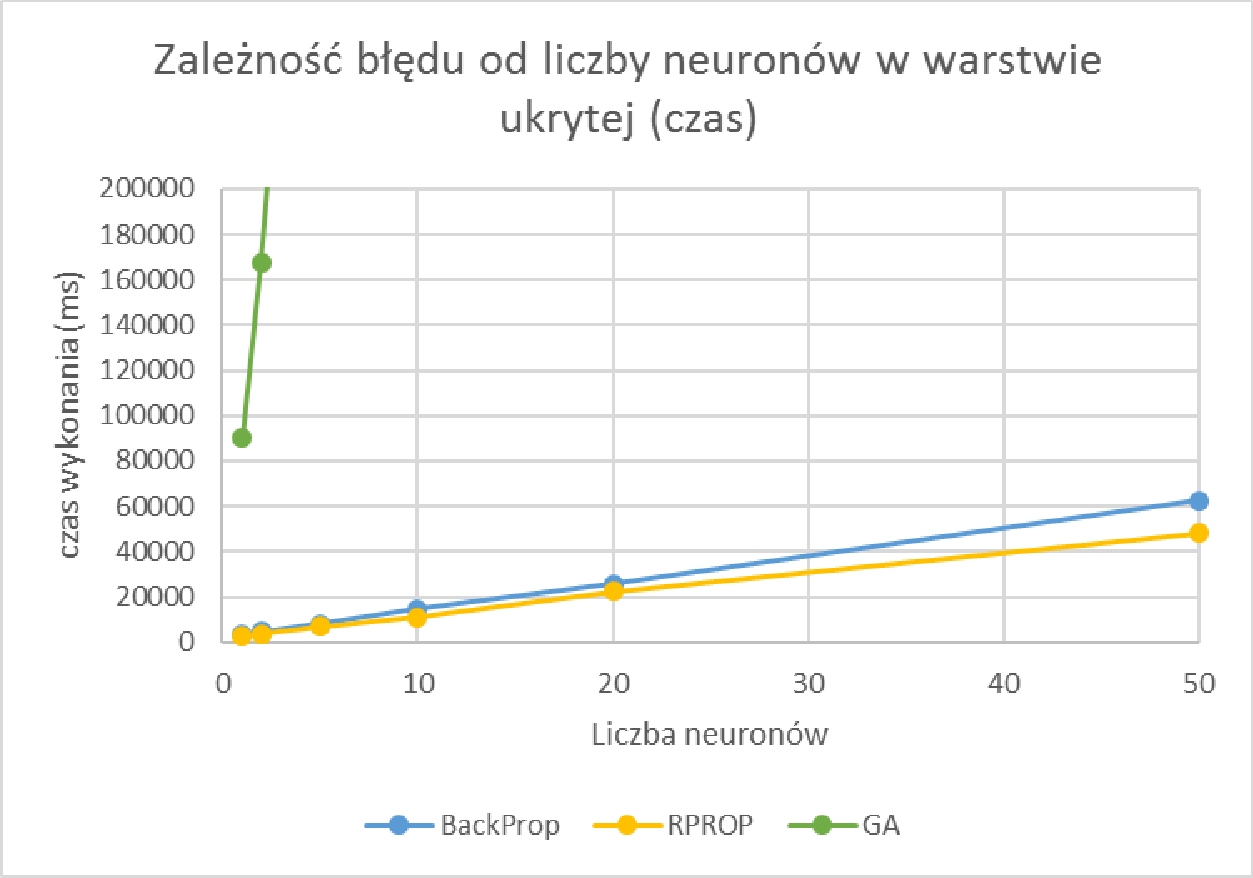
\includegraphics[width=0.7\textwidth]{am_exphiddenneural_time}
					\caption{Wyniki eksperymentu testującego optymalny rozmiar ukrytej warstwy neuronów na bazie AmazonMeta. Wykres przedstawia zależność pomiędzy ilością neuronów a~czasem wykonania. Czas wykonania rośnie liniowo proporcjonalnie do ilości neuronów. W~związku z~tym oraz biorąc pod uwagę wykres \ref{fig:am_exphiddenneural_rmse} optymalnym jest ustalenie liczby neuronów w~warstwie ukrytej na 1.}
					\label{fig:am_exphiddenneural_time}
				\end{figure}
	
				\begin{longtable}{r||rr|rr|rr}
					\label{tab:am_exphiddenneural}
					\centering
					\textbf{L. neuronów} &  \multicolumn{2}{c|}{\textbf{Propagacja wsteczna}}  & \multicolumn{2}{c|}{\textbf{RPROP}} & \multicolumn{2}{c}{\textbf{Alg. genetyczny}}  \\
					\hline
					& \textbf{RMSE} & \textbf{czas} & \textbf{RMSE} & \textbf{czas} & \textbf{RMSE} & \textbf{czas} \\
					\hline
					1  & 0.936219 & 3817  & 0.930452 & 2854  & 0.930968 & 89939   \\
					2  & 0.935587 & 4680  & 0.930152 & 3629  & 0.930092 & 167708  \\
					5  & 0.933983 & 7947  & 0.929796 & 6977  & 0.930443 & 471038  \\
					10 & 1.171907 & 14826 & 0.930305 & 11182 & 0.930253 & 651918  \\
					20 & 1.32946  & 25576 & 0.930192 & 22295 & 0.930148 & 937888  \\
					50 & 1.32946  & 62574 & 1.32946  & 48140 & 0.92978  & 2055270 \\	
					\caption{Zależność błędu algorytmu RMSE i~czasu wykonania od rozmiaru ukrytej warstwy neuronowej (baza AmazonMeta).}
				\end{longtable}
			
			\subsubsection{Podsumowanie}
		
			Bazując na przeprowadzonych eksperymentach zostały zdefiniowane optymalne parametry algorytmu filtrowania z~analizą zawartości. Zostały one przedstawione w~tabeli \ref{tab:am_optimummovielens}.
			
			\begin{center}
				\begin{longtable}{ | R{7cm}   m{8cm} |}
					\hline				
					\multicolumn{2}{|c|}{\textbf{Optymalna konfiguracja filtrowania z~analizą zawartości dla bazy AmazonMeta}} \\
					\hline
					Maksymalna ilość iteracji nauki: & 1000 \\				
					Współczynnik bezwładności: & 0 \\
					Rozmiar populacji: & 50 \\
					Ilość neuronów w~warstwie ukrytej: & 1 \\
					Współczynnik uczenia: & 0.1 \\
					Parametr funkcji aktywacji $\alpha$: & 2.0 \\						
					\hline
					\caption{Konfiguracja dla eksperymentu dopasowania rozmiaru ukrytej warstwy neuronów (baza AmazonMeta).}
					\label{tab:am_optimummovielens}
				\end{longtable}
			\end{center}
		
		\section{Eksperymentalne porównanie zaproponowanych algorytmów hybrydowych z~filtrowaniem z~analizą zawartości i~filtrowaniem kolaboratywnym}
		
		Eksperymenty miały na celu porównanie efektywności zaproponowanych algorytmów hybrydowych z~samym filtrowaniem kolaboratywnym i~z samym filtrowaniem z~analizą zawartości. Początkowo zostały przeprowadzone testy odrębnie dla filtrowania kolaboratywnego i~dla filtrowania z~analizą zawartości. Następnie dla takiej samej konfiguracji parametrów zostały uruchomione algorytmy hybrydowe. 
		
		Parametrami, które ulegały modyfikacji były parametr określający minimum powtarzających się cech ocenianych elementów i~liczba użytkowników brana pod uwagę przez filtrowanie kolaboratywne. Sieć neuronowa została skonfigurowana w~sposób wynikający z~eksperymentów przeprowadzonych w~rozdziałach \ref{ss:strojeniemovielens} i~\ref{ss:strojenieamazonmeta}.
		
		Dla każdego algorytmu hybrydowego wykonanych zostało 12 pomiarów. Parametr określający minimalną liczbę powtarzających się cech przyjmował wartości 1, 2 i~5. Parametr określający liczbę użytkowników braną pod uwagę podczas budowania macierzy użytkownik-element w~kolaboratywnej części składowej algorytmu przyjmował wartości 50, 100, 500, 1000. 
		
		Przyjęto następującą metodologię: algorytm hybrydowy zawsze porównywany był z~filtrowaniem z~analizą zawartości o~analogicznym sposobie uczenia sieci neuronowej. Tak też algorytm hybrydowy typu ,,matrix factorization i~sieć neuronowa uczona metodą propagacji wstecznej'' porównany jest z~algorytmem filtrowania z~analizą zawartości z~siecią neuronową uczoną metodą propagacji wstecznej.
		
		\subsection{Badania na bazie MovieLens}
				
		\subsubsection{Porównanie algorytmów hybrydowych z~filtrowaniem z~analizą zawartości}
		
		W pierwszej kolejności porównany został algorytm hybrydowy typu matrix  factorization i~sieć neuronowa uczona metodą propagacji wstecznej. Wyniki eksperymentu przedstawia rys. \ref{fig:ml_exphybrid1_1}. Zgodnie z~oczekiwaniami im większa macierz użytkownik-element tym lepsze były uzyskane rezultaty. W~przypadku uwzględnieniu 100 użytkowników otrzymane rezultaty były gorsze niż te uzyskane metodą filtrowania z~analizą zawartości. Jednakże przy uwzględnieniu 200 użytkowników i~więcej wynik był znacznie lepszy. 
		
		\begin{figure}
			\centering
			\includegraphics[width=0.7\textwidth]{ml_exphybrid1_1}			
			\caption{Wyniki eksperymentu porównującego działanie algorytmu hybrydowego ,,matrix factorization i~sieć neuronowa uczona metodą propagacji wstecznej'' z~filtrowaniem z~analizą zawartości z~siecią neuronową uczoną metodą propagacji wstecznej (baza MovieLens).}
			\label{fig:ml_exphybrid1_1}
		\end{figure}
	
		Kolejnym porównywanym algorytmem był algorytm hybrydowy ,,biased matrix factorization i~sieć neuronowa uczona metodą propagacji wstecznej''. Wyniki eksperymentu przedstawia rys. \ref{fig:ml_exphybrid1_2}. 
		W tym wypadku uwzględnienie tylko 100 użytkowników w~komponencie filtrowania kolaboratywnego powodowało osiąganie lepszego rezultatu. Pomiędzy RMSE a~liczbą użytkowników występuje tendencja spadkowa. W~tym eksperymencie nastąpiło niewielkie zaburzenie tej tendencji (na granicy błędu statystycznego) w~przypadku 2 i~5 powtarzających się cech dla 1000 i~2000 użytkowników. Ponadto, wyniki osiągnięte przez ten algorytm hybrydowy są nieco lepsze niż przez algorytm hybrydowy ,,matrix factorization i~sieć neuronowa uczona metodą propagacji wstecznej''.
	
		\begin{figure}
			\centering
			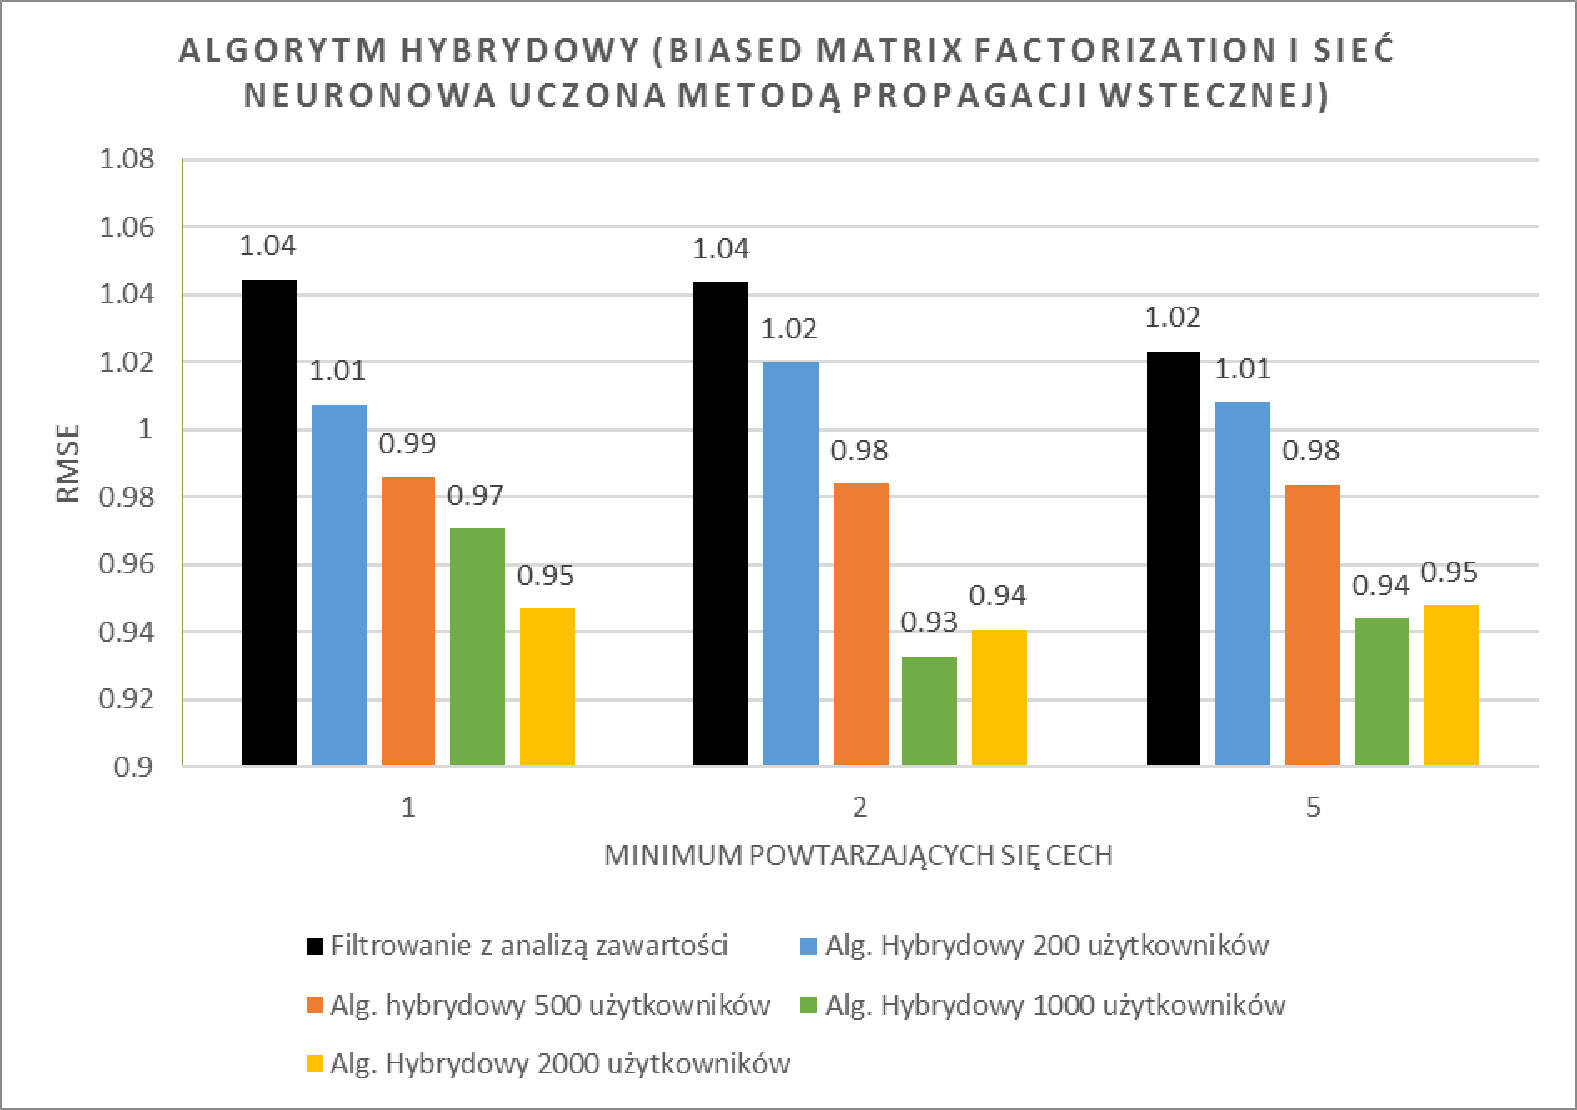
\includegraphics[width=0.7\textwidth]{ml_exphybrid1_2}			
			\caption{Wyniki eksperymentu porównującego działanie algorytmu hybrydowego ,,biased matrix factorization i~sieć neuronowa uczona metodą propagacji wstecznej'' z~filtrowaniem z~analizą zawartości z~siecią neuronową uczoną metodą propagacji wstecznej (baza MovieLens).}
			\label{fig:ml_exphybrid1_2}
		\end{figure}
		
		Rys. \ref{fig:ml_exphybrid1_3} przedstawia porównanie algorytmu hybrydowego ,,SVD++ i~sieć neuronowa uczona metodą propagacji wstecznej'' z~filtrowaniem z~analizą zawartości z~siecią neuronową uczoną metodą propagacji wstecznej. Warto zauważyć, że wyniki osiągnięte przez taki algorytm są niewiele gorsze lub identyczne z~wynikami osiągniętymi przez algorytm z~poprzedniego porównania. 

		\begin{figure}
			\centering
			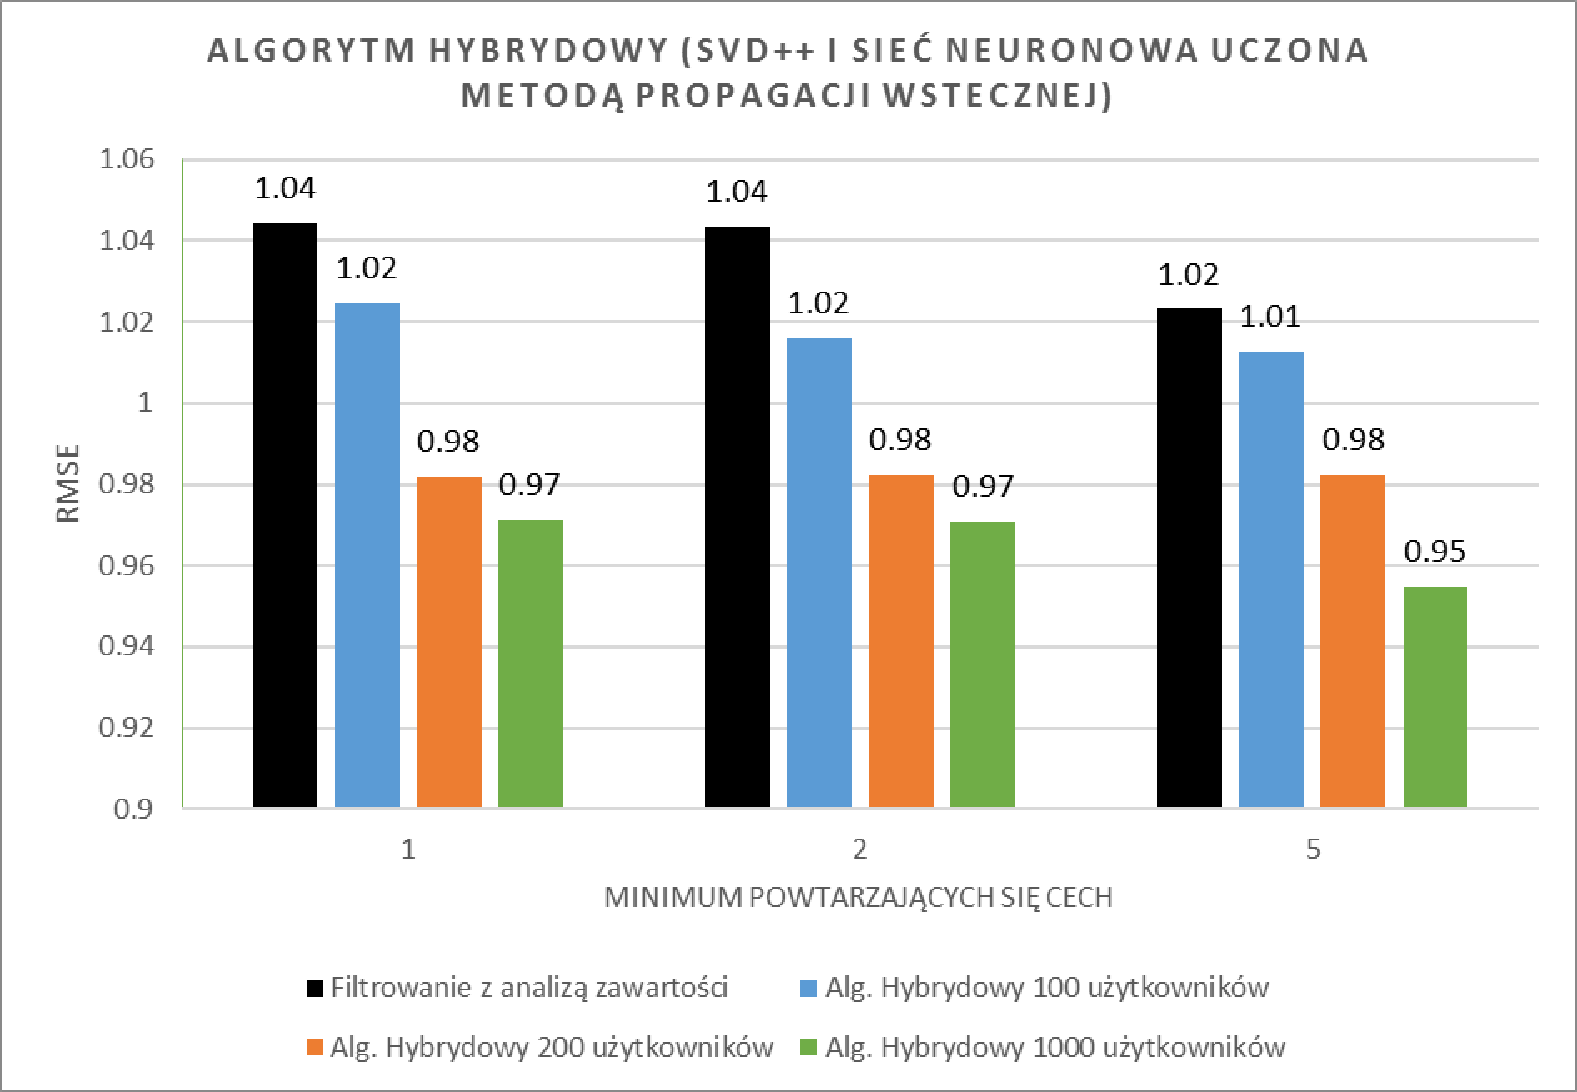
\includegraphics[width=0.7\textwidth]{ml_exphybrid1_3}			
			\caption{Wyniki eksperymentu porównującego działanie algorytmu hybrydowego ,,SVD++ i~sieć neuronowa uczona metodą propagacji wstecznej'' z~filtrowaniem z~analizą zawartości z~siecią neuronową uczoną metodą propagacji wstecznej (baza MovieLens).}
			\label{fig:ml_exphybrid1_3}
		\end{figure}
		
		Następne trzy wykresy: rys. \ref{fig:ml_exphybrid1_4}, rys. \ref{fig:ml_exphybrid1_5} i~rys. \ref{fig:ml_exphybrid1_6} przedstawiają porównanie kolejno algorytmów hybrydowych ,,matrix factorization i~sieć neuronowa uczona metodą RPROP'', ,,biased matrix factorization i~sieć neuronowa uczona metodą RPROP'' i~,,SVD++ i~sieć neuronowa uczona metodą RPROP'' z~filtrowaniem z~analizą zawartości z~siecią neuronową uczoną metodą RPROP. Tak jak w~poprzednich przypadkach można zauważyć, że rezultaty są za każdym razem lepsze a~skuteczność rośnie wraz ze wzrostem wielkości macierzy użytkownik-element.
		
		Największa niespodzianka występuje w~przypadku testu porównującego działanie algorytmu hybrydowego ,,SVD++ i~sieć neuronowa uczona metodą RPROP'' (rys. \ref{fig:ml_exphybrid1_6}). Dla 200 użytkowników został osiągnięty dużo lepszy wynik niż dla 1000 użytkowników. Takie zjawisko występuje jednak tylko w~przypadku 1 powtarzającej się cechy. Dla 2 i~5 osiągnięte wyniki są bardziej zbliżone do przewidywanych. Jako, że taka sytuacja wystąpiła tylko raz można założyć, że wynika to z~niefortunnie dobranych danych, dla których zbudowanie rekomendacji okazało się być trudniejsze niż zazwyczaj. 
		
		Warto też zauważyć, że zgodnie z~wcześniejszymi oczekiwaniami, algorytm filtrowania z~analizą zawartości z~siecią neuronową uczoną metodą RPROP zwraca sporo gorsze wyniki niż analogiczny algorytm uczony metodą propagacji wstecznej (odpowiednio $RMSE \in \{1,02; 1,02; 1,01\}$ i~$RMSE \in \{1,38; 1,18; 1,04\}$ dla 1, 2 i~5 powtarzających się cech). 
		
		\begin{figure}
			\centering
			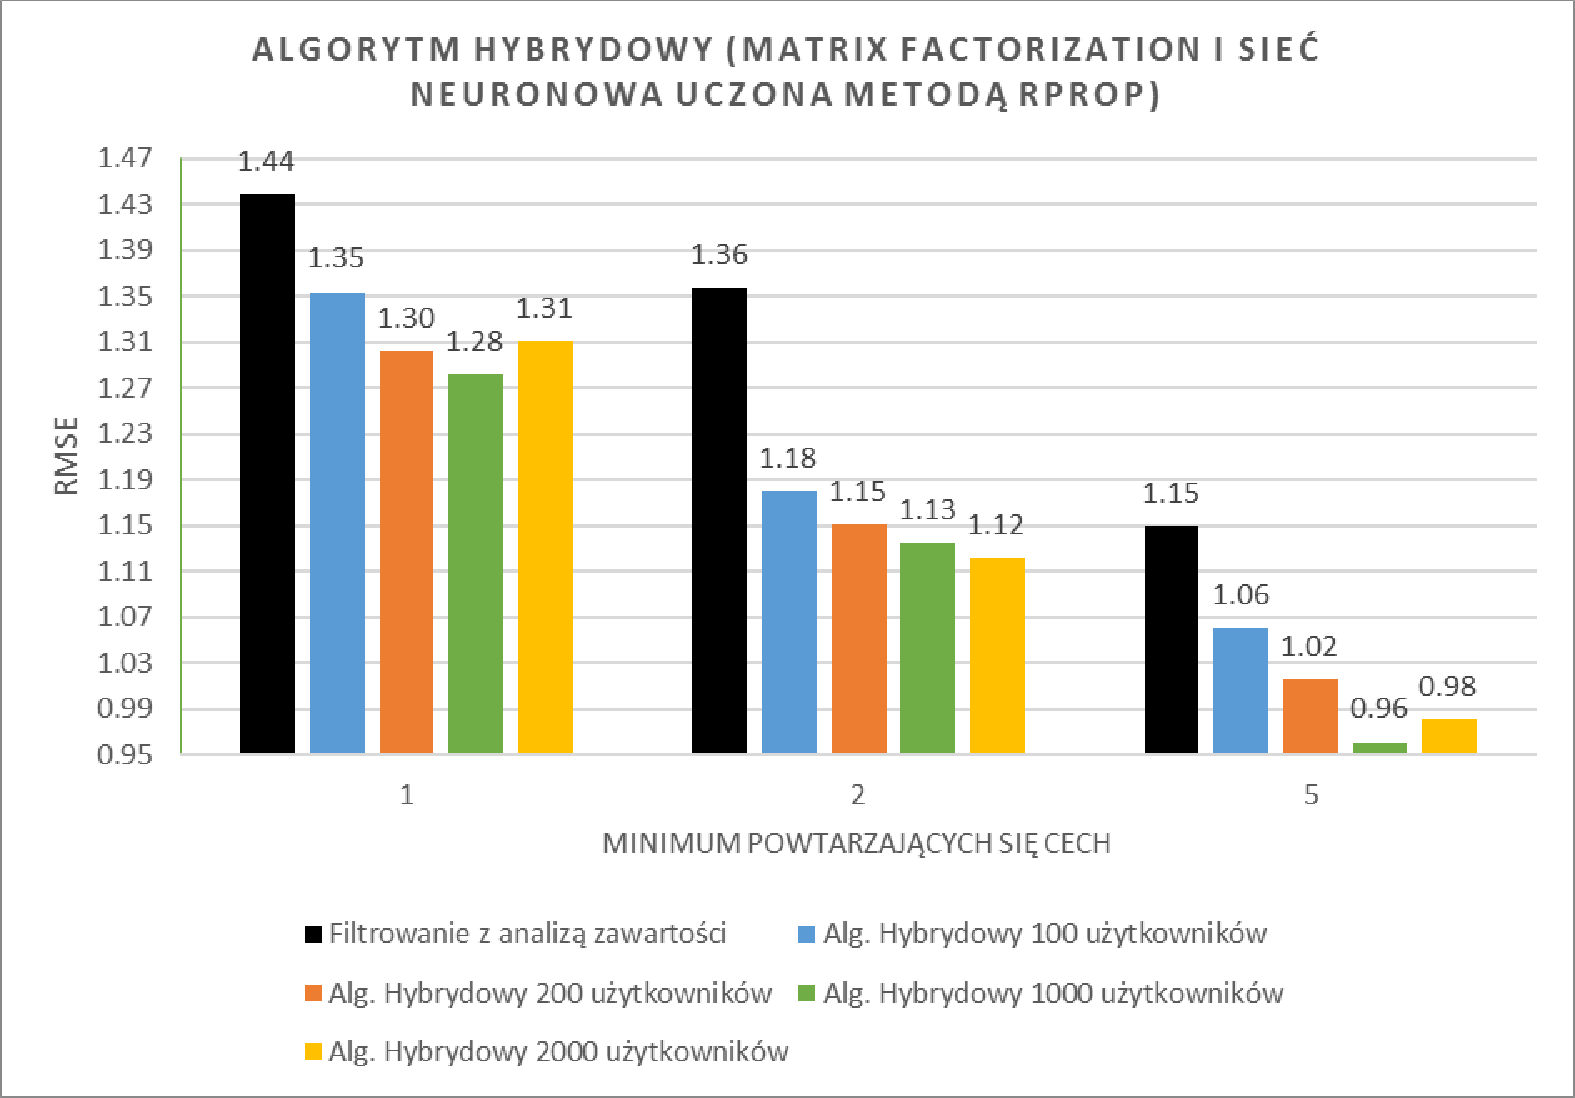
\includegraphics[width=0.7\textwidth]{ml_exphybrid1_4}			
			\caption{Wyniki eksperymentu porównującego działanie algorytmu hybrydowego ,,matrix factorization i~sieć neuronowa uczona metodą RPROP'' z~filtrowaniem z~analizą zawartości z~siecią neuronową uczoną metodą RPROP (baza MovieLens).}
			\label{fig:ml_exphybrid1_4}
		\end{figure}
	
		\begin{figure}
			\centering
			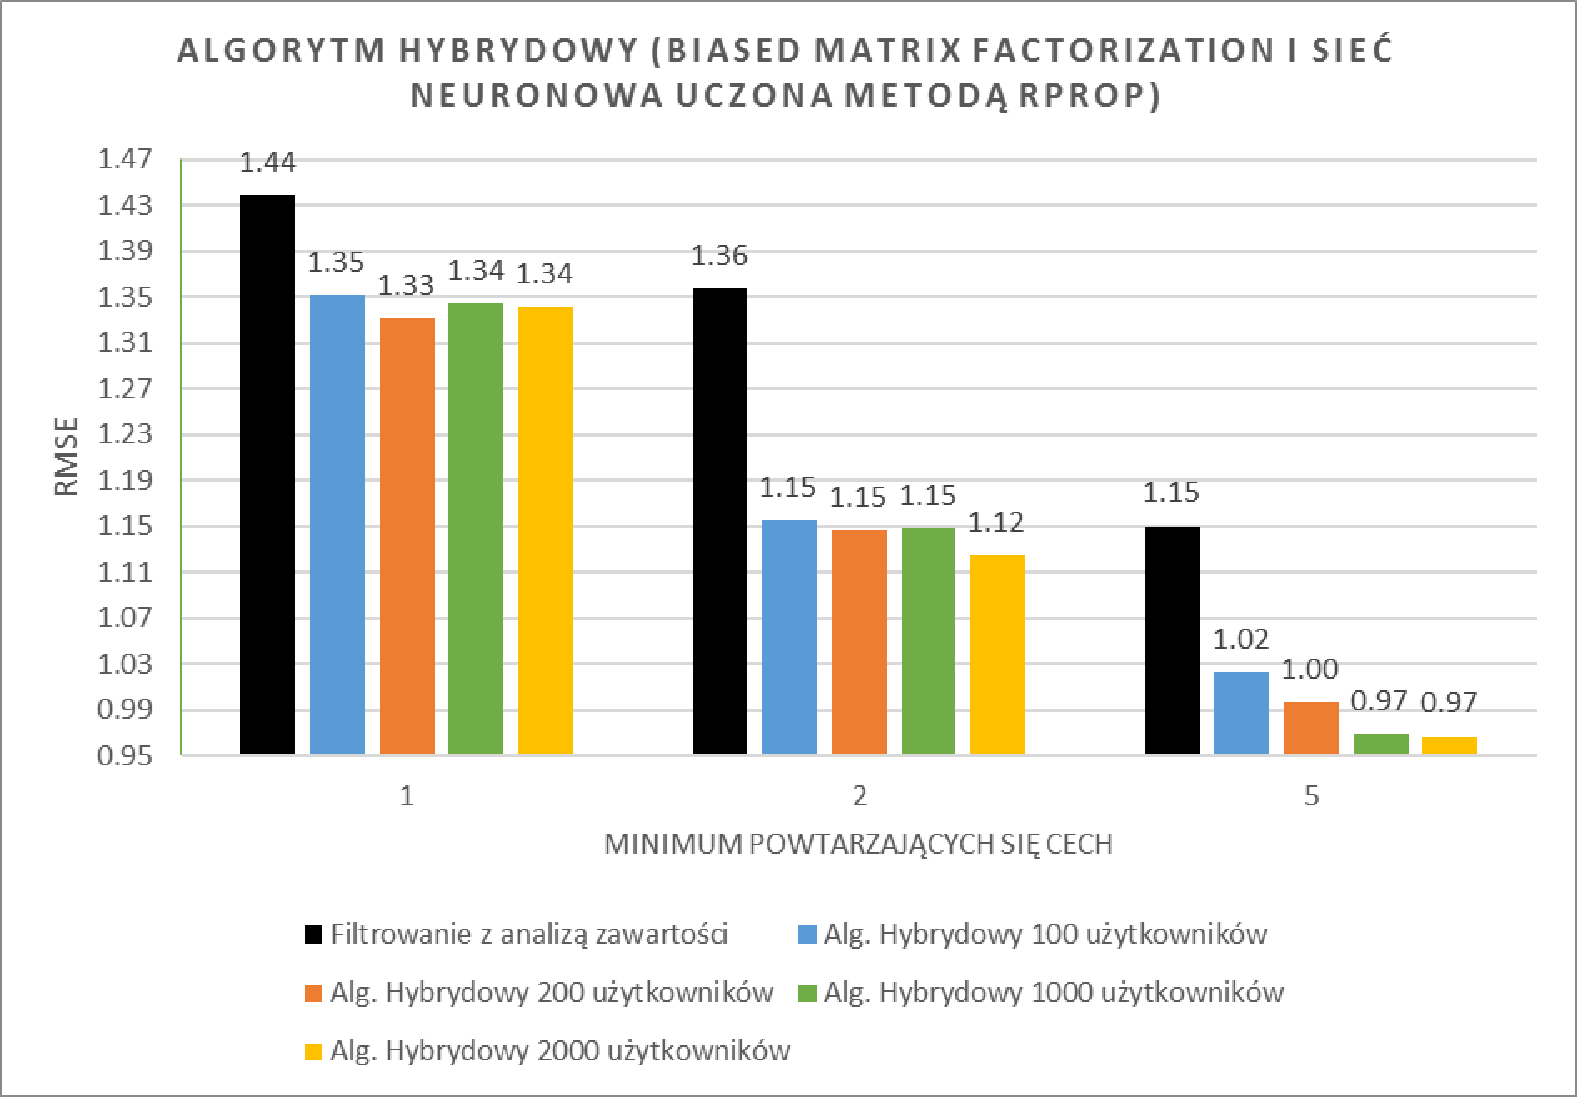
\includegraphics[width=0.7\textwidth]{ml_exphybrid1_5}			
			\caption{Wyniki eksperymentu porównującego działanie algorytmu hybrydowego ,,biased matrix factorization i~sieć neuronowa uczona metodą RPROP'' z~filtrowaniem z~analizą zawartości z~siecią neuronową uczoną metodą RPROP (baza MovieLens).}
			\label{fig:ml_exphybrid1_5}
		\end{figure}
		
		\begin{figure}
			\centering
			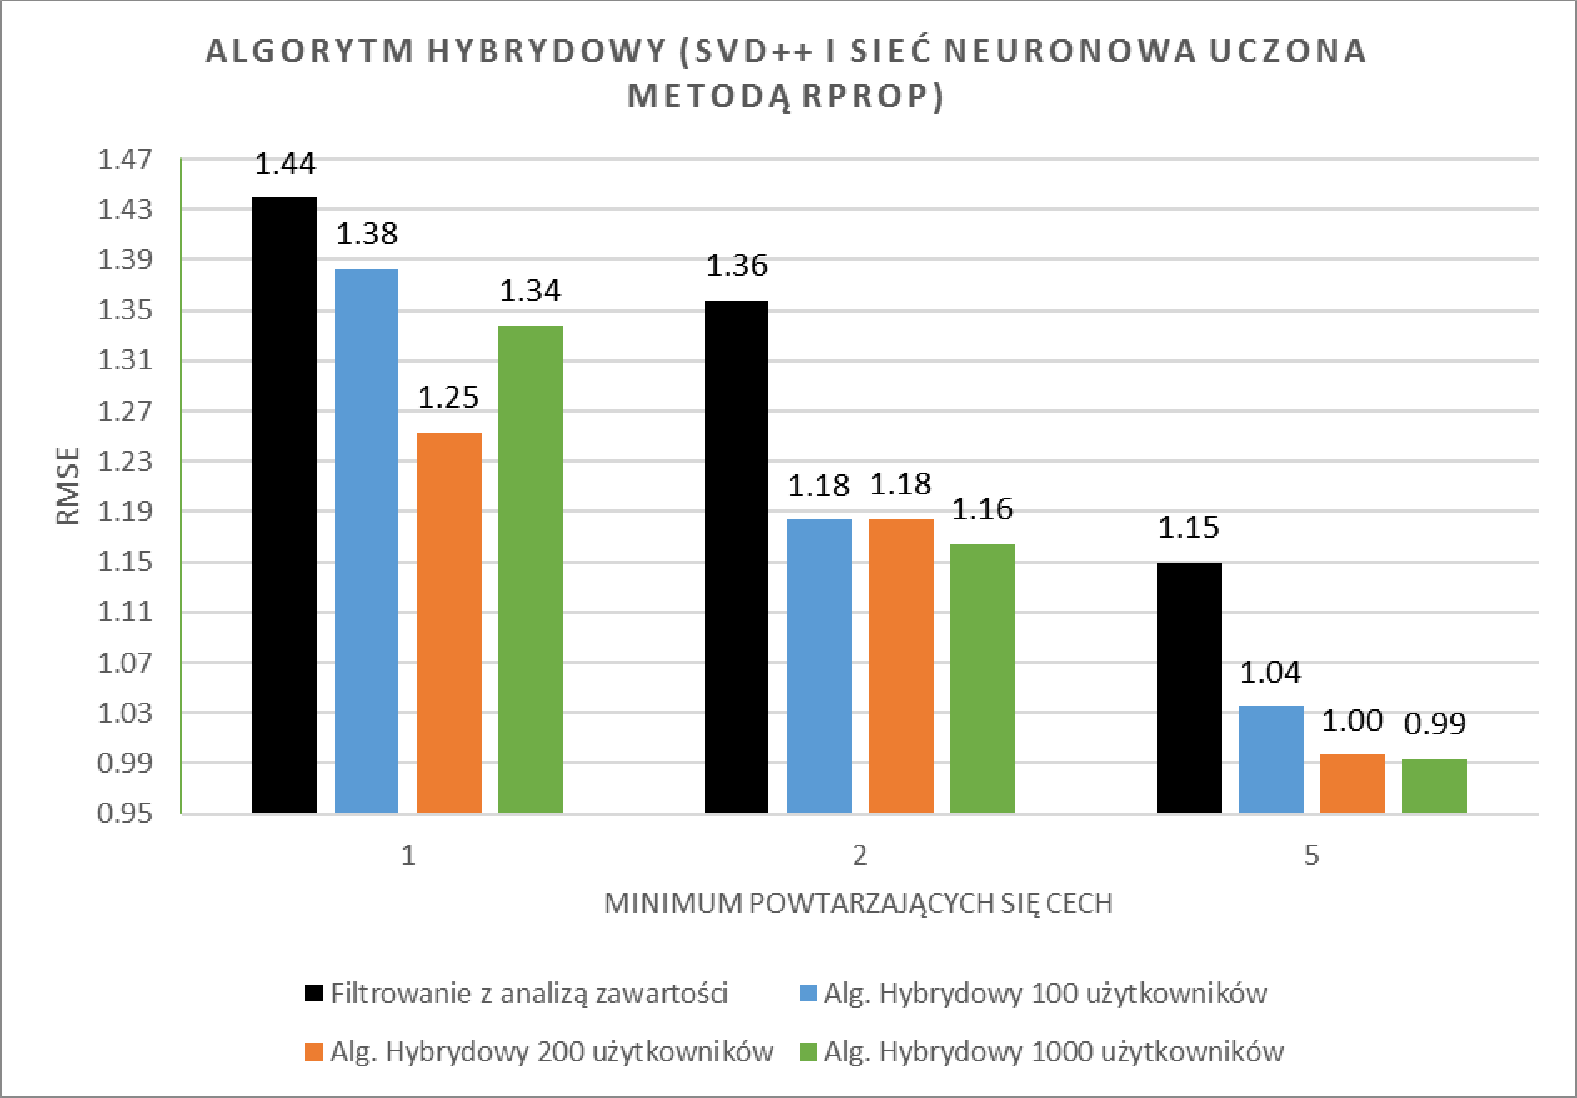
\includegraphics[width=0.7\textwidth]{ml_exphybrid1_6}			
			\caption{Wyniki eksperymentu porównującego działanie algorytmu hybrydowego ,,SVD++ i~sieć neuronowa uczona metodą RPROP'' z~filtrowaniem z~analizą zawartości z~siecią neuronową uczoną metodą RPROP (baza MovieLens).}
			\label{fig:ml_exphybrid1_6}
		\end{figure}
		
		Ostatnie trzy wykresy: rys. \ref{fig:ml_exphybrid1_7}, rys. \ref{fig:ml_exphybrid1_8} i~rys. \ref{fig:ml_exphybrid1_9} przedstawiają porównanie kolejno algorytmów hybrydowych ,,matrix factorization i~sieć neuronowa uczona algorytmem genetycznym'', ,,biased matrix factorization i~sieć neuronowa uczona algorytmem genetycznym'' i~,,SVD++ i~sieć neuronowa uczona algorytmem genetycznym'' z~filtrowaniem z~analizą zawartości z~siecią neuronową uczoną algorytmem genetycznym.
		
		Wyniki osiągnięte przez algorytm genetyczny są nieznacznie gorsze niż te osiągnięte przez metodę propagacji wstecznej. Poza tym, zgodnie z~oczekiwaniami występuje ujemna korelacja pomiędzy ilością użytkowników a~RMSE.
		
			\begin{figure}
			\centering
			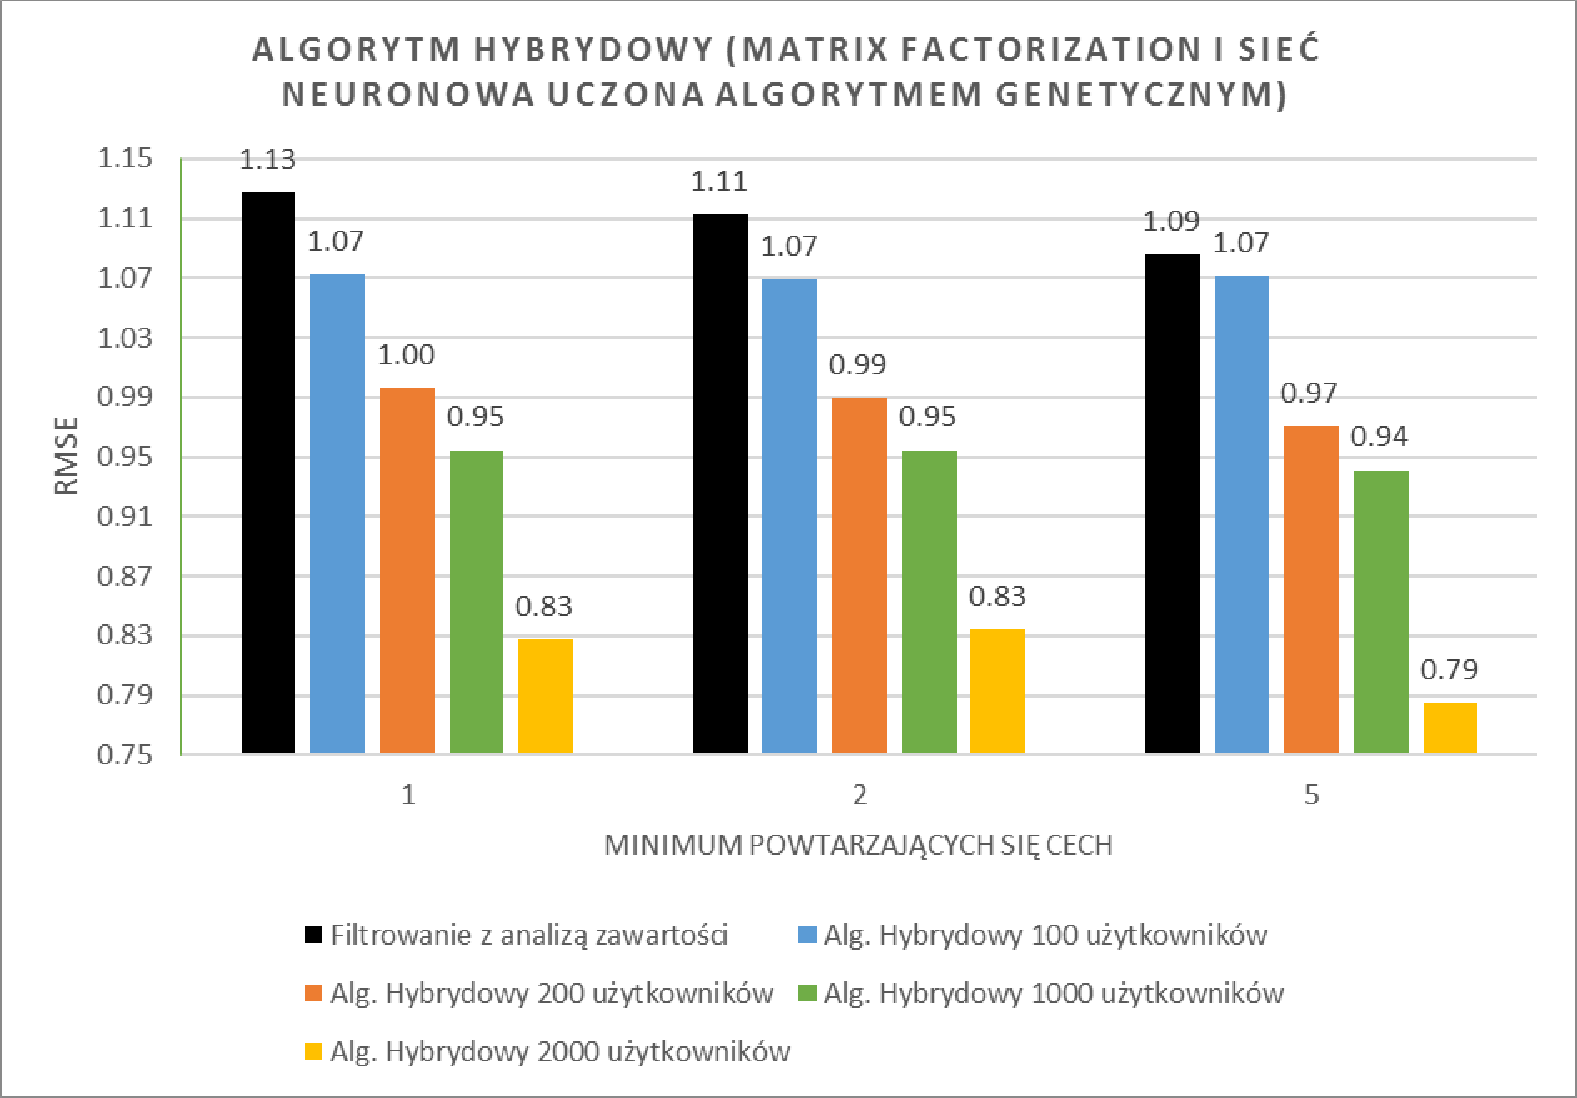
\includegraphics[width=0.7\textwidth]{ml_exphybrid1_7}			
			\caption{Wyniki eksperymentu porównującego działanie algorytmu hybrydowego ,,matrix factorization i~sieć neuronowa uczona metodą algorytmem genetycznym'' z~filtrowaniem z~analizą zawartości z~siecią neuronową uczoną algorytmem genetycznym (baza MovieLens).}
			\label{fig:ml_exphybrid1_7}
		\end{figure}
		
		\begin{figure}
			\centering
			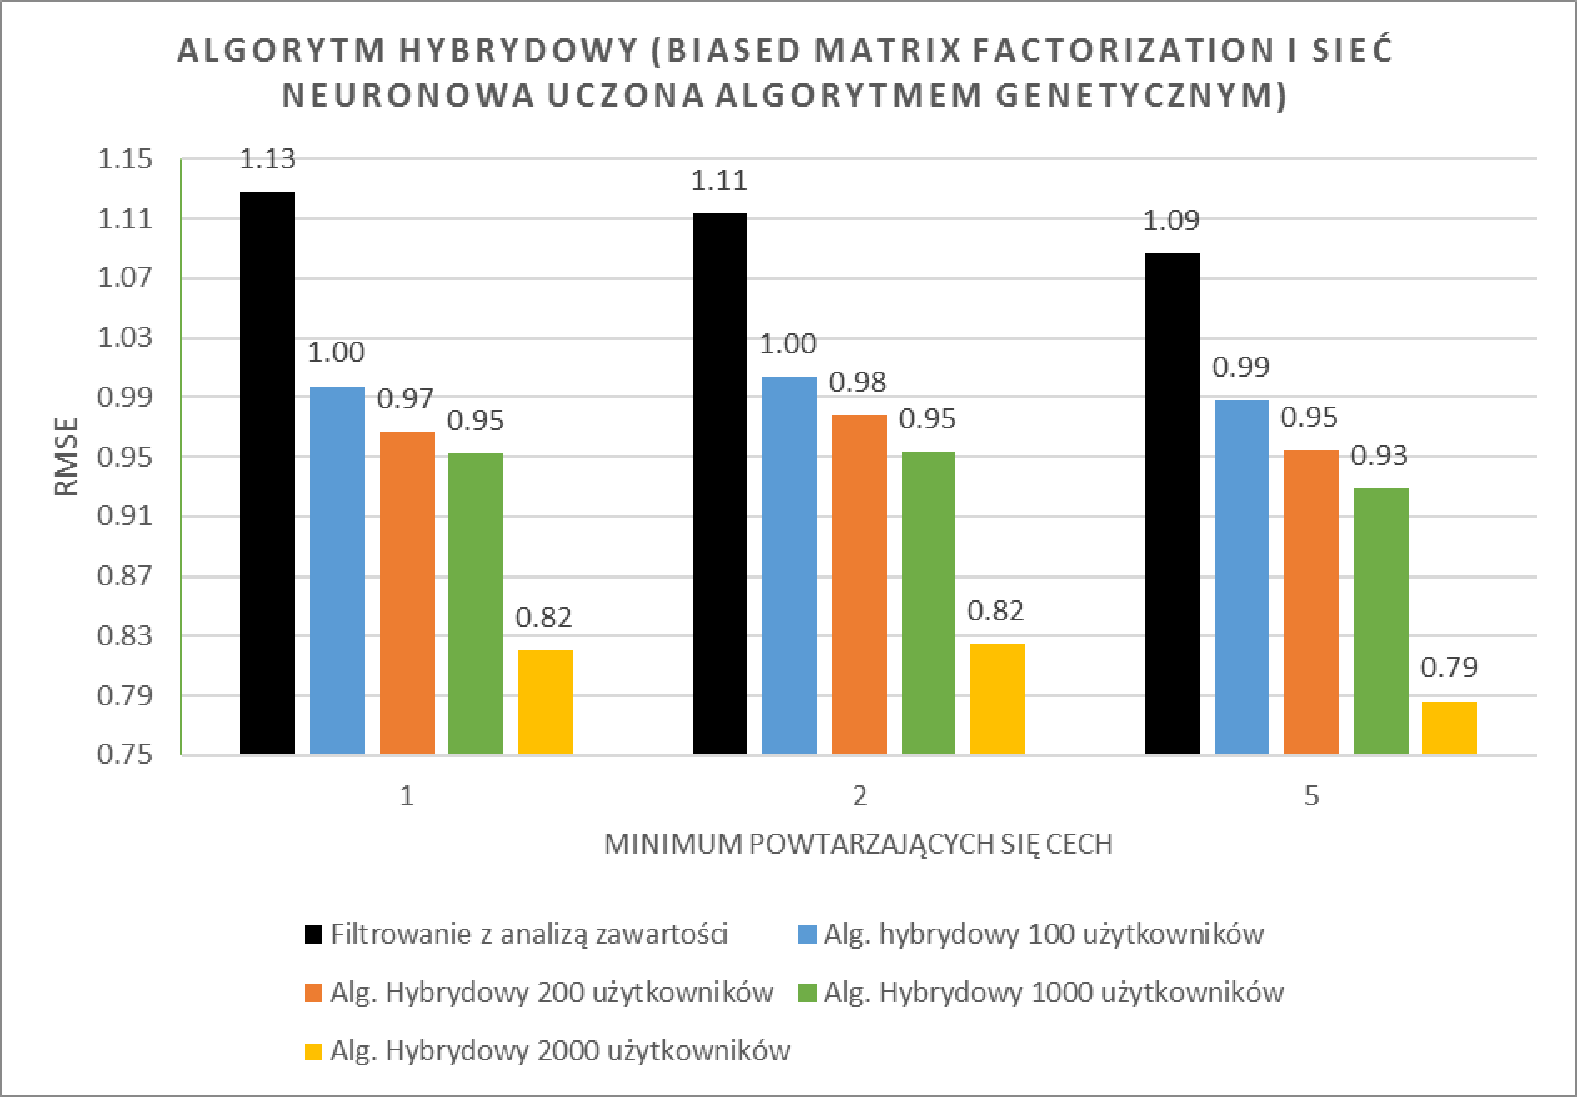
\includegraphics[width=0.7\textwidth]{ml_exphybrid1_8}			
			\caption{Wyniki eksperymentu porównującego działanie algorytmu hybrydowego ,,biased matrix factorization i~sieć neuronowa uczona algorytmem genetycznym'' z~filtrowaniem z~analizą zawartości z~siecią neuronową uczoną algorytmem genetycznym (baza MovieLens).}
			\label{fig:ml_exphybrid1_8}
		\end{figure}
		
		\begin{figure}
			\centering
			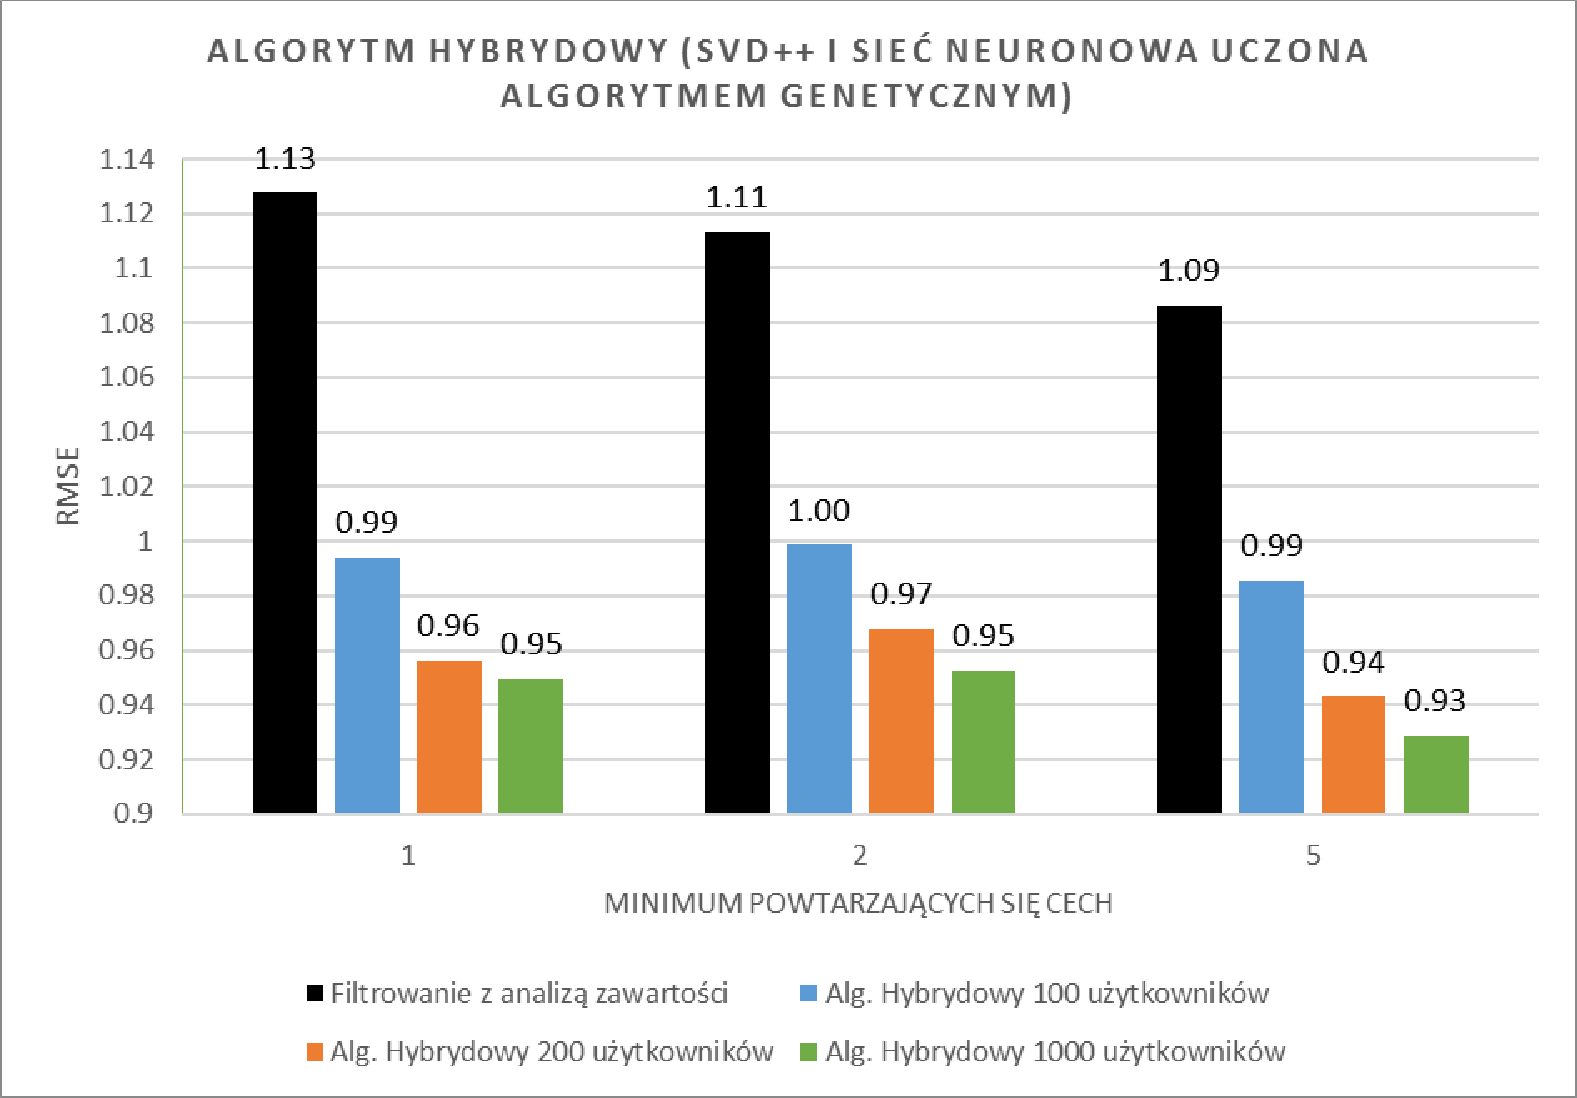
\includegraphics[width=0.7\textwidth]{ml_exphybrid1_9}			
			\caption{Wyniki eksperymentu porównującego działanie algorytmu hybrydowego ,,SVD++ i~sieć neuronowa uczona metodą RPROP'' z~algorytmem genetycznym'' z~filtrowaniem z~analizą zawartości z~siecią neuronową uczoną algorytmem genetycznym (baza MovieLens).}
			\label{fig:ml_exphybrid1_9}
		\end{figure}
	
		Podsumowując, w~przypadku bazy danych MovieLens, pomijając pierwszy przypadek, już 100 użytkowników okazało się być wystarczająco wysoką liczbą aby wykorzystanie algorytmu hybrydowego wpływało pozytywnie na efekt końcowy. Ponadto, zgodnie z~oczekiwaniami występuje wyraźna korelacja ujemna pomiędzy liczbą użytkowników a~RMSE. 
		
		Liczba powtarzających się cech nieznacznie wpłynęła na wynik w~przypadku zastosowania algorytmu filtrowania z~analizą zawartości z~siecią neuronową uczoną metodą propagacji wstecznej, jednak w~przypadku sieci uczonej metodą RPROP różnica była znaczna. 
		
		Najlepszy rezultat osiągnięty został dzięki zastosowaniu algorytmu hybrydowego ,,biased matrix factorization i~sieć neuronowa uczona algorytmem genetycznym'' i~,,biased matrix factorization i~sieć neuronowa uczona algorytmem genetycznym'' dla 5 powtarzających się cech i~2000 użytkowników. RMSE wyniosło $0,79$.
		
		\subsubsection{Porównanie algorytmów hybrydowych z~filtrowaniem kolaboratywnym}
		
		Wykresy \ref{fig:ml_exphybrid2_1} i~\ref{fig:ml_exphybrid2_2} przedstawiają porównanie algorytmów hybrydowych z~filtrowaniem kolaboratywnym metodą matrix factorization. W~przypadku algorytmu hybrydowego ,,matrix factorization i~sieć neuronowa uczona metodą propagacji wstecznej'' i~,,matrix factorization i~sieć neuronowa uczona metodą RPROP'' można zaobserwować ujemną korelację pomiędzy liczbą powtarzających się cech a~RMSE. Algorytm ,,matrix factorization i~sieć neuronowa uczona algorytmem genetycznym'' radzi sobie dużo gorzej z~elementami o~5 powtarzających się cechach niż 1 lub 2. Poza algorytmem hybrydowym ,,matrix factorization i~sieć neuronowa uczona metodą RPROP'' radzą sobie one lepiej niż czysty algorytm filtrowania kolaboratywnego metodą matrix factorization.
		
		Wykresy \ref{fig:ml_exphybrid2_2} i~\ref{fig:ml_exphybrid2_3} przedstawiają porównanie algorytmów hybrydowych z~filtrowaniem kolaboratywnym metodą biased matrix factorization. Podobnie jak poprzednio algorytmy hybrydowe o~składowej filtrowania z~analizą treści metodą propagacji wstecznej i~algorytmem genetycznym radzą sobie lepiej. Algorytm o~składowej RPROP wypada znacznie gorzej niż samo filtrowanie kolaboratywne w~przypadku 1 powtarzającej się cechy. Dopiero uwzględnienie co najmniej 5 cech pozwala na uzyskanie lepszych rezultatów.
		
		Wykresy \ref{fig:ml_exphybrid2_4} i~\ref{fig:ml_exphybrid2_5} przedstawiają porównanie algorytmów hybrydowych z~filtrowaniem kolaboratywnym metodą SVD++. Występuje analogiczna sytuacja jak wcześniej podczas zastosowaniu składowej filtrowania z~analizą treści metodą RPROP. Poza tym tendencje są podobne do poprzednich przypadków.
		
		\begin{figure}
			\centering
			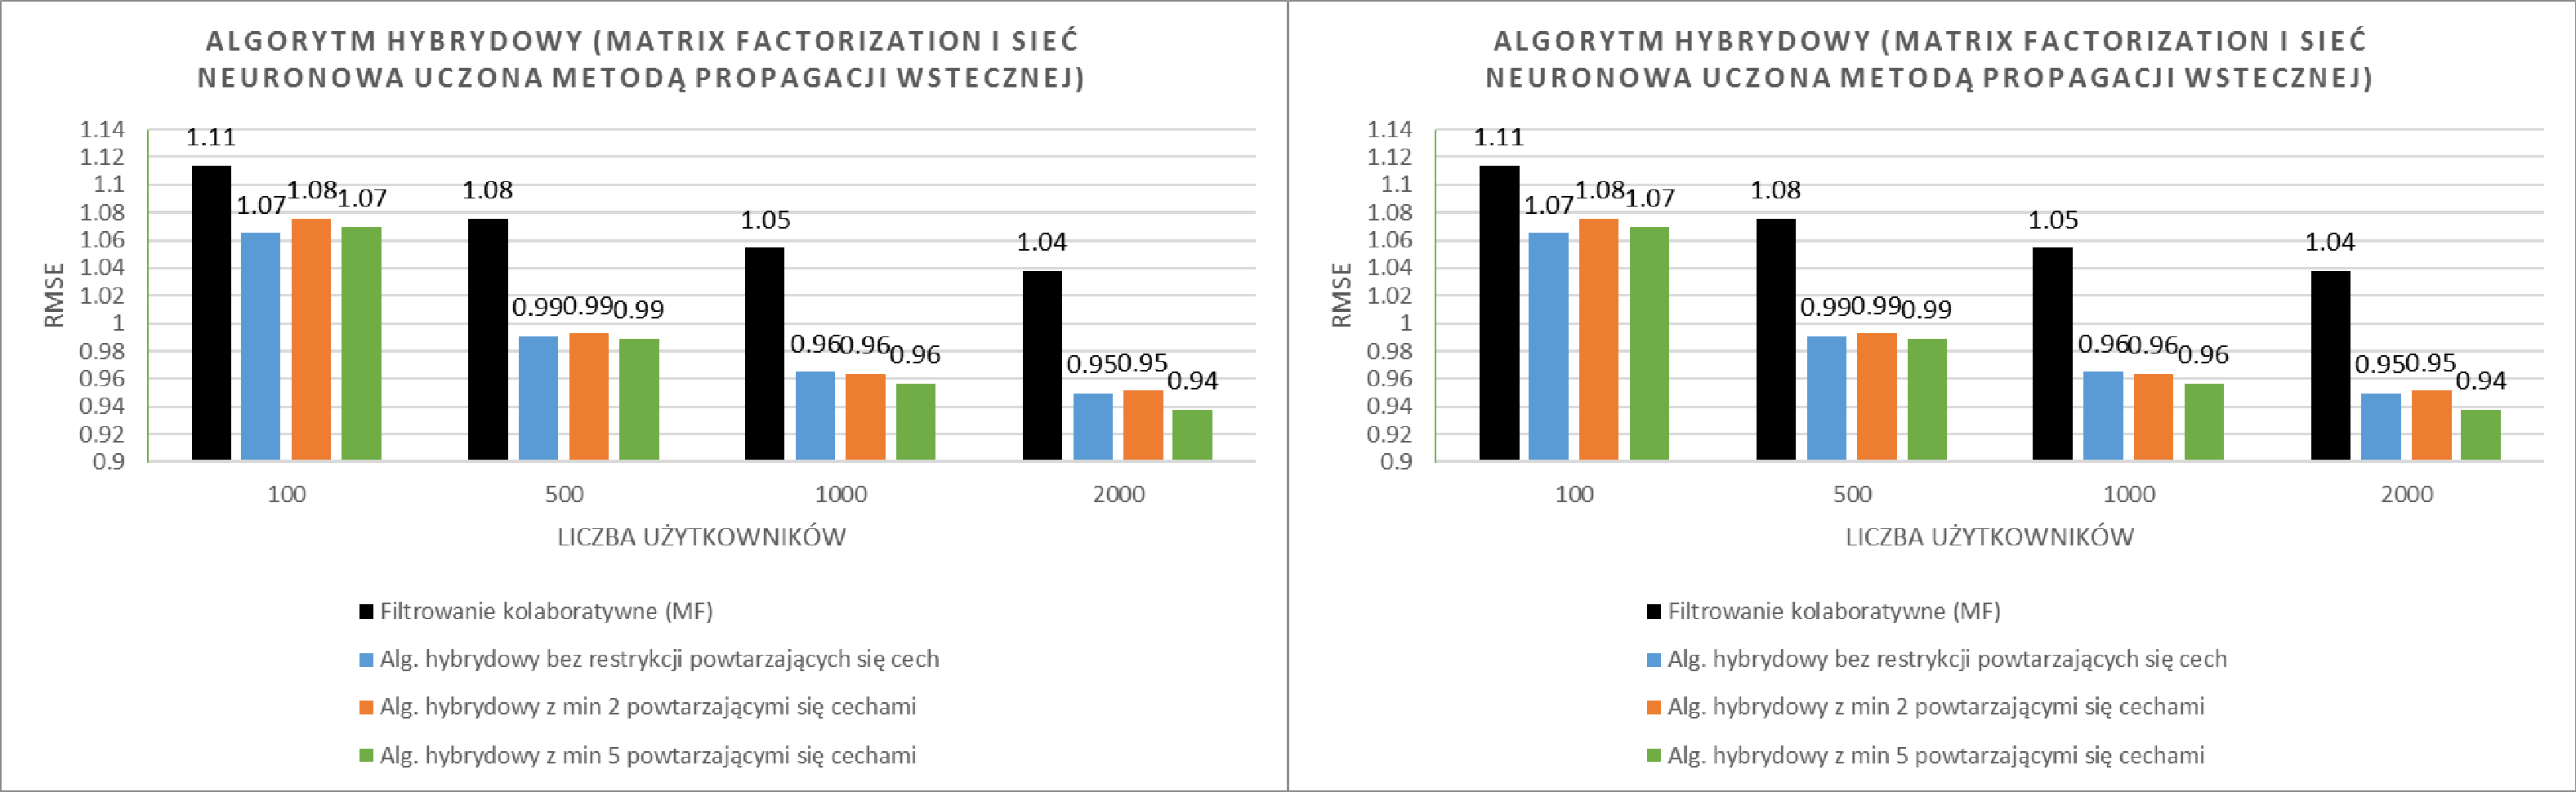
\includegraphics[width=1\textwidth]{ml_exphybrid2_1}			
			\caption{\textbf{Po lewej}: wyniki eksperymentu porównującego działanie algorytmu hybrydowego ,,matrix factorization i~sieć neuronowa uczona metodą propagacji wstecznej'' z~filtrowaniem kolaboratywnym metodą ,,matrix factorization''. \textbf{Po prawej}: wyniki eksperymentu porównującego działanie algorytmu hybrydowego ,,matrix factorization i~sieć neuronowa uczona metodą RPROP'' z~filtrowaniem kolaboratywnym metodą ,,matrix factorization'' (baza MovieLens).}
			\label{fig:ml_exphybrid2_1}
		\end{figure}
		
		\begin{figure}
			\centering
			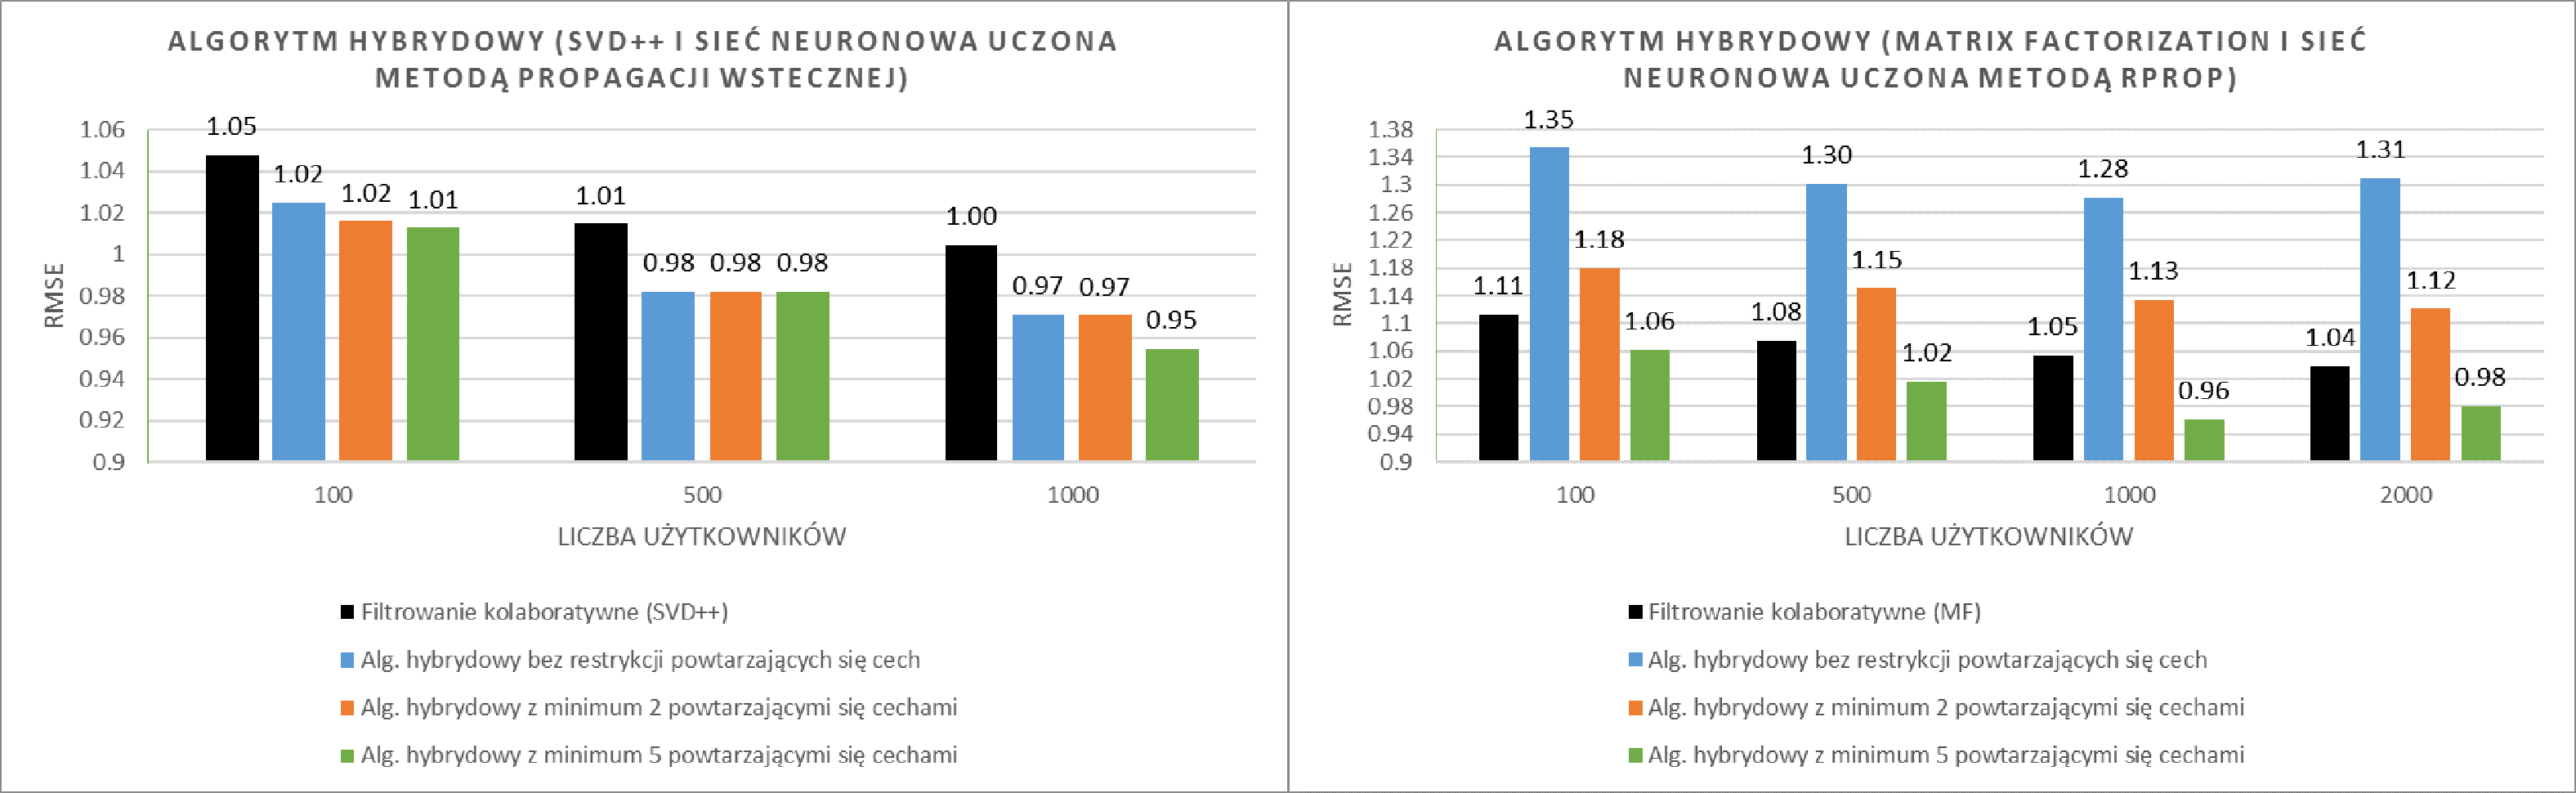
\includegraphics[width=1\textwidth]{ml_exphybrid2_2}			
			\caption{\textbf{Po lewej}: wyniki eksperymentu porównującego działanie algorytmu hybrydowego ,,matrix factorization i~sieć neuronowa uczona algorytmem genetycznym'' z~filtrowaniem kolaboratywnym metodą ,,matrix factorization''. \textbf{Po prawej}: wyniki eksperymentu porównującego działanie algorytmu hybrydowego ,,biased matrix factorization i~sieć neuronowa uczona metodą propagacji wstecznej'' z~filtrowaniem kolaboratywnym metodą ,,biased matrix factorization'' (baza MovieLens).}
			\label{fig:ml_exphybrid2_2}
		\end{figure}
		
		\begin{figure}
			\centering
			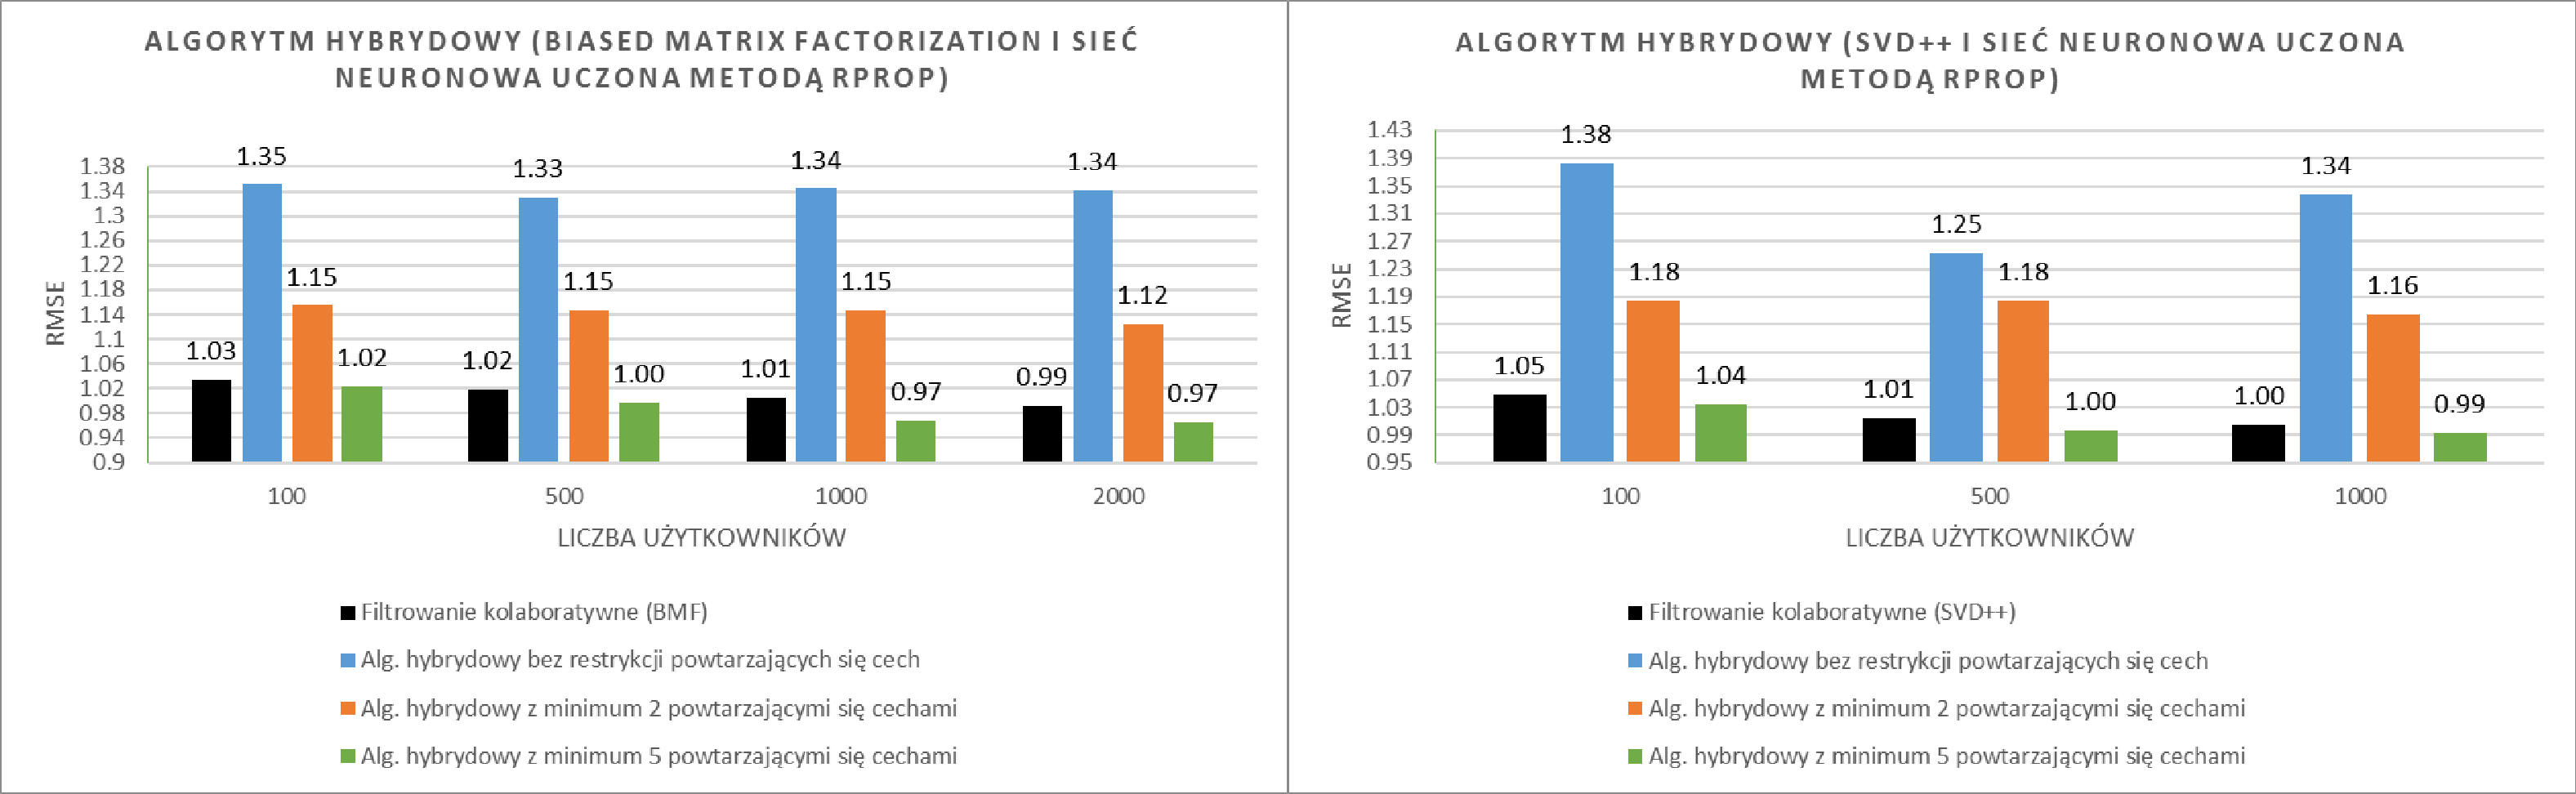
\includegraphics[width=1\textwidth]{ml_exphybrid2_3}			
			\caption{\textbf{Po lewej}: wyniki eksperymentu porównującego działanie algorytmu hybrydowego ,,biased matrix factorization i~sieć neuronowa uczona metodą RPROP'' z~filtrowaniem kolaboratywnym metodą ,,biased matrix factorization''. \textbf{Po prawej}: wyniki eksperymentu porównującego działanie algorytmu hybrydowego ,,biased matrix factorization i~sieć neuronowa uczona algorytmem genetycznym'' z~filtrowaniem kolaboratywnym metodą ,,biased matrix factorization''(baza MovieLens).}
			\label{fig:ml_exphybrid2_3}
		\end{figure}
		
		\begin{figure}
			\centering
			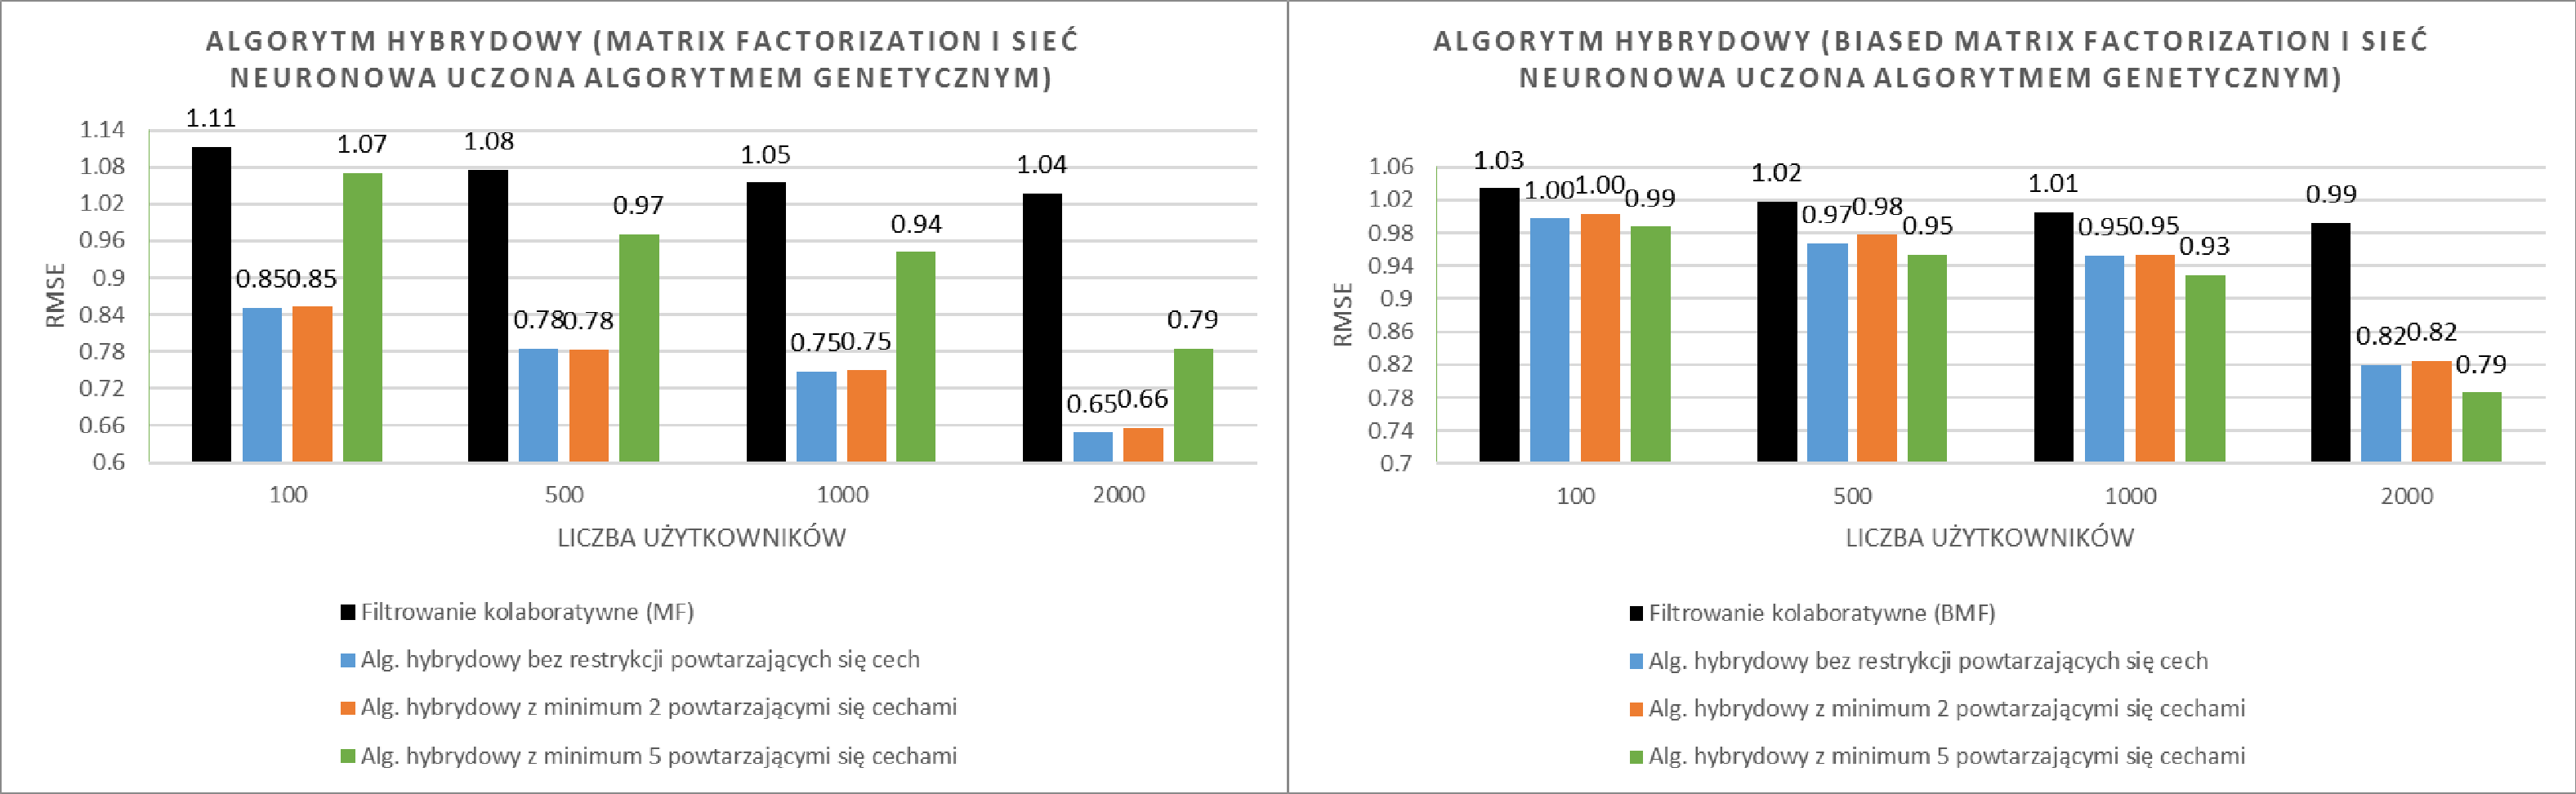
\includegraphics[width=1\textwidth]{ml_exphybrid2_4}			
			\caption{\textbf{Po lewej}: wyniki eksperymentu porównującego działanie algorytmu hybrydowego ,,SVD++ i~sieć neuronowa uczona metodą propagacji wstecznej'' z~filtrowaniem kolaboratywnym metodą ,,SVD++''. \textbf{Po prawej}: wyniki eksperymentu porównującego działanie algorytmu hybrydowego ,,SVD++ i~sieć neuronowa uczona metodą RPROP'' z~filtrowaniem kolaboratywnym metodą ,,SVD++'' (baza MovieLens).}
			\label{fig:ml_exphybrid2_4}
		\end{figure}
		
		\begin{figure}
			\centering
			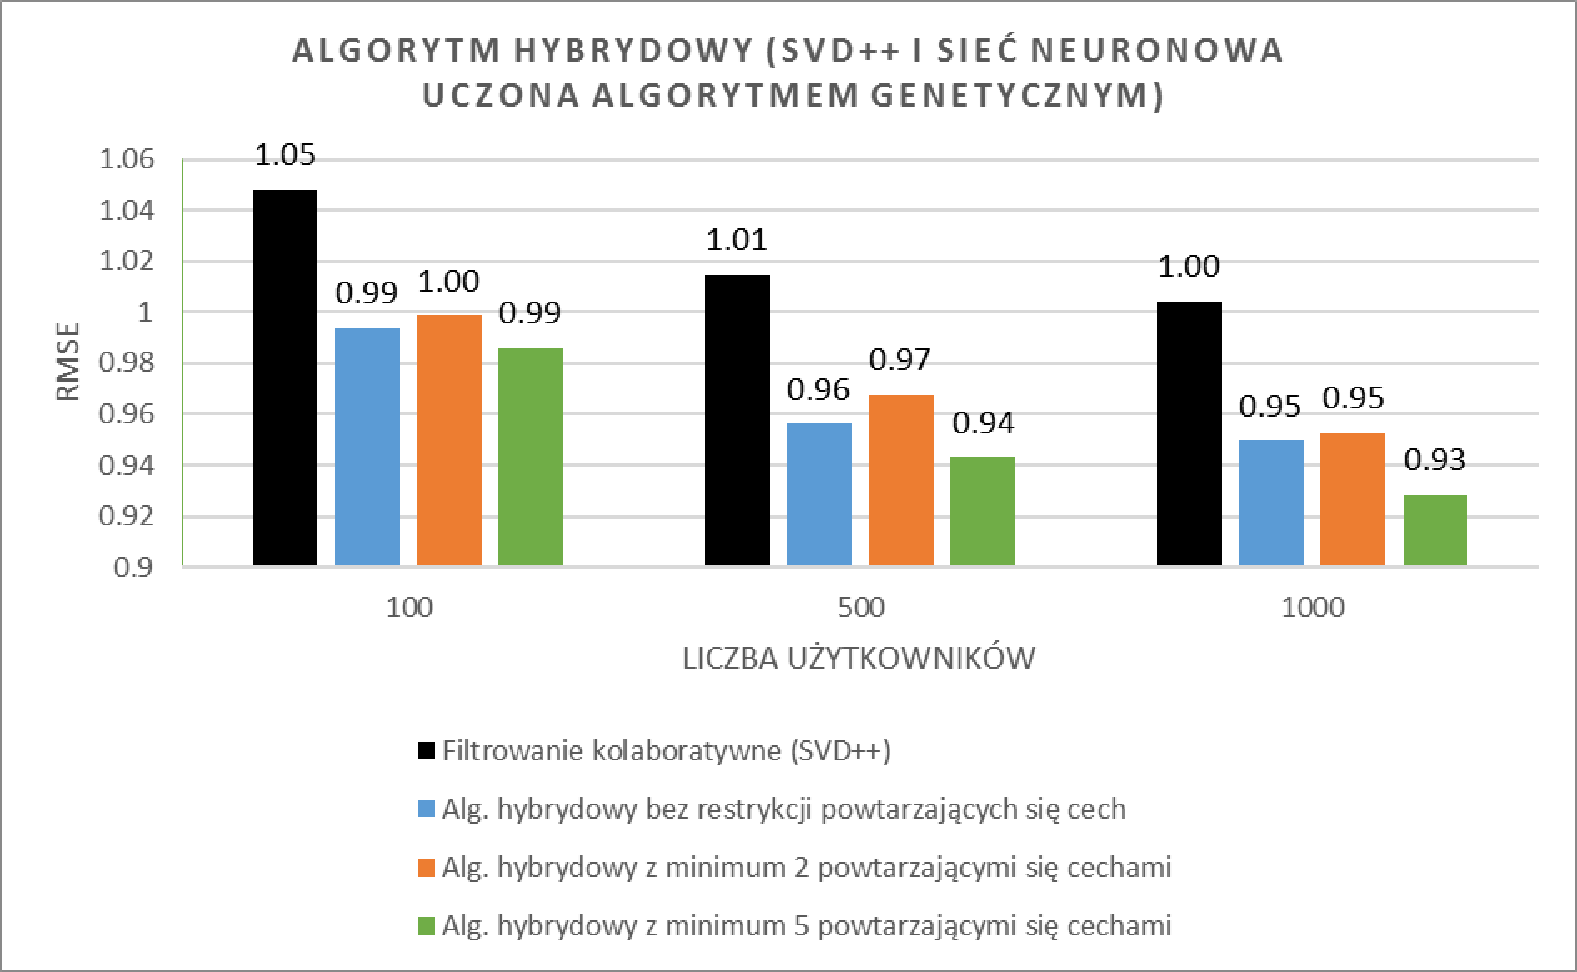
\includegraphics[width=0.5\textwidth]{ml_exphybrid2_5}			
			\caption{Wyniki eksperymentu porównującego działanie algorytmu hybrydowego ,,SVD++ i~sieć neuronowa uczona algorytmem genetycznym'' z~filtrowaniem kolaboratywnym metodą ,,SVD++'' (baza MovieLens).}
			\label{fig:ml_exphybrid2_5}
		\end{figure}
	
		\subsubsection{Porównanie uśrednionych wartości}
		
		Aby porównać efektywność poszczególnych algorytmów otrzymane wyniki zostały uśrednione. Rezultat przedstawia wykres \ref{fig:ml_exphybrid}. Najlepsze rezultaty otrzymane zostały dzięki algorytmowi hybrydowemu ,,biased matrix factorization i~sieć neuronowa uczona algorytmem genetycznym". W~porównaniu do rezultatu osiągniętego za pomocą filtrowania z~analizą zawartości (RPROP) RMSE zmalało o~ $29,36\%$. W~porównaniu do najefektywniejszego algorytmu nie-hybrydowego, algorytmu filtrowania kolaboratywnego (biased matrix factorization) RMSE zmalało o~$8,82\%$.
		
		\begin{figure}
			\centering
			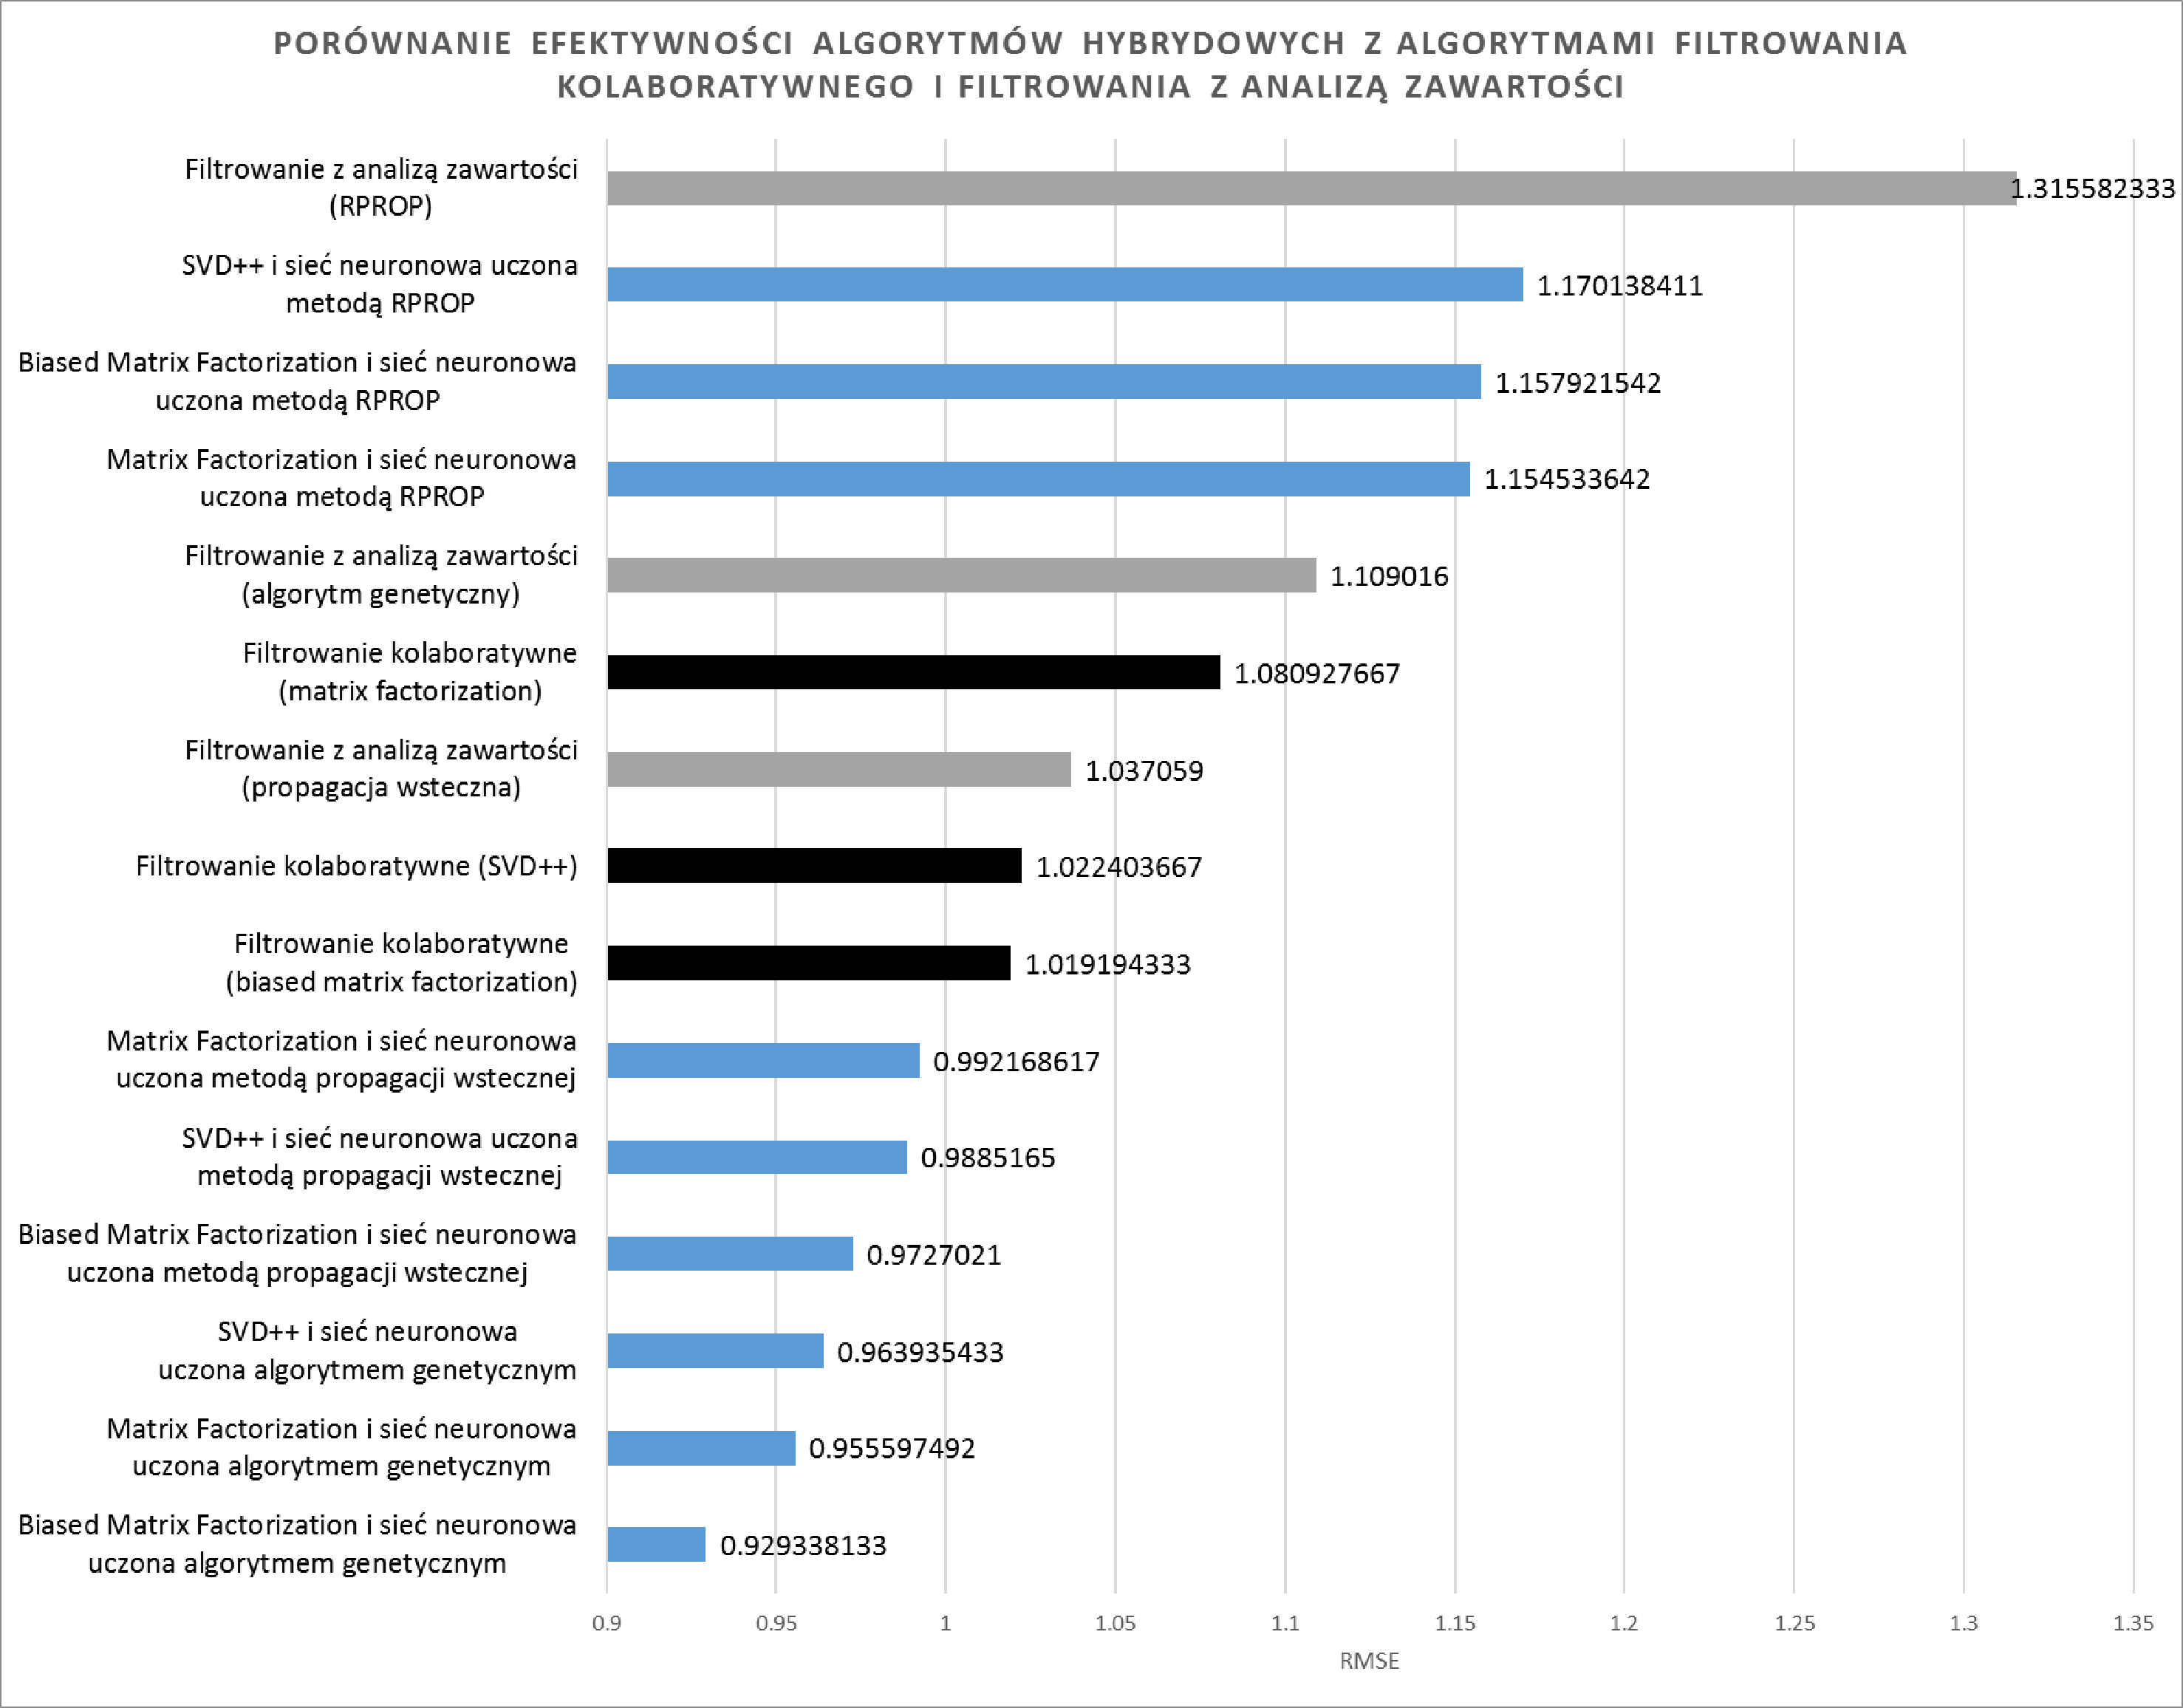
\includegraphics[width=1\textwidth]{ml_exphybrid}	
			\caption{Wykres przedstawia porównanie wyników działania algorytmów hybrydowych (słupki niebieskie) z~algorytmami filtrowania kolaboratywnego (słupki czarne) i~filtrowania z~analizą zawartości (słupki szare) (baza MovieLens).}
			\label{fig:ml_exphybrid}
		\end{figure}
		
		\subsection{Badania na bazie AmazonMeta}
				
		\subsubsection{Porównanie algorytmów hybrydowych z~filtrowaniem z~analizą zawartości}
		
		Badania na bazie AmazonMeta zostały przeprowadzone w~sposób analogiczny do tych przeprowadzonych na bazie MovieLens. Wyniki eksperymentów przedstawiają rys. \ref{fig:am_exphybrid1_1}, \ref{fig:am_exphybrid1_2}, \ref{fig:am_exphybrid1_3}, \ref{fig:am_exphybrid1_4} i~ \ref{fig:am_exphybrid1_5}.
		
		W przypadku tej bazy danych dużo lepiej wypadły algorytmy hybrydowe, nawet dla konfiguracji z~zaledwie 50 użytkownikami. Nieznacznie lepiej od pozostałych wypadała konfiguracja z~minimum dwoma powtarzającymi się cechami. Dla wszystkich algorytmów hybrydowych można zauważyć delikatną tendencję spadkową wartości RMSE wraz ze wzrostem liczby użytkowników uwzględnianych w~składowej filtrowania kolaboratywnego, za wyjątkiem tych które wykorzystują metodę SVD++. Algorytmy hybrydowe o~składowej filtrowania kolaboratywnego bazującej na metodzie SVD++ wykazały takie same (lub prawie takie same o~różnicy na poziomie błędu statystycznego) wyniki wartości RMSE.
		
		Najlepsze wyniki dla tej bazy danych zostały osiągnięte dzięki algorytmom: ,,biased matrix factorization i~sieć neuronowa uczona algorytmem genetycznym'' i~,,biased matrix factorization i~sieć neuronowa uczona metodą propagacji wstecznej'', warto jednak zauważyć że różnica pomiędzy kolejnymi wynikami algorytmów hybrydowych jest bardzo nieznaczna. 
		
		\begin{figure}
			\centering
			\includegraphics[width=1\textwidth]{am_exphybrid1_1}			
			\caption{\textbf{Po lewej}: wyniki eksperymentu porównującego działanie algorytmu hybrydowego ,,matrix factorization i~sieć neuronowa uczona metodą propagacji wstecznej'' z~filtrowaniem z~analizą zawartości z~siecią neuronową uczoną metodą propagacji wstecznej. \textbf{Po prawej}: wyniki eksperymentu porównującego działanie algorytmu hybrydowego ,,biased matrix factorization i~sieć neuronowa uczona metodą propagacji wstecznej'' z~filtrowaniem z~analizą zawartości z~siecią neuronową uczoną metodą propagacji wstecznej (baza AmazonMeta).}
			\label{fig:am_exphybrid1_1}
		\end{figure}
		
		\begin{figure}
			\centering
			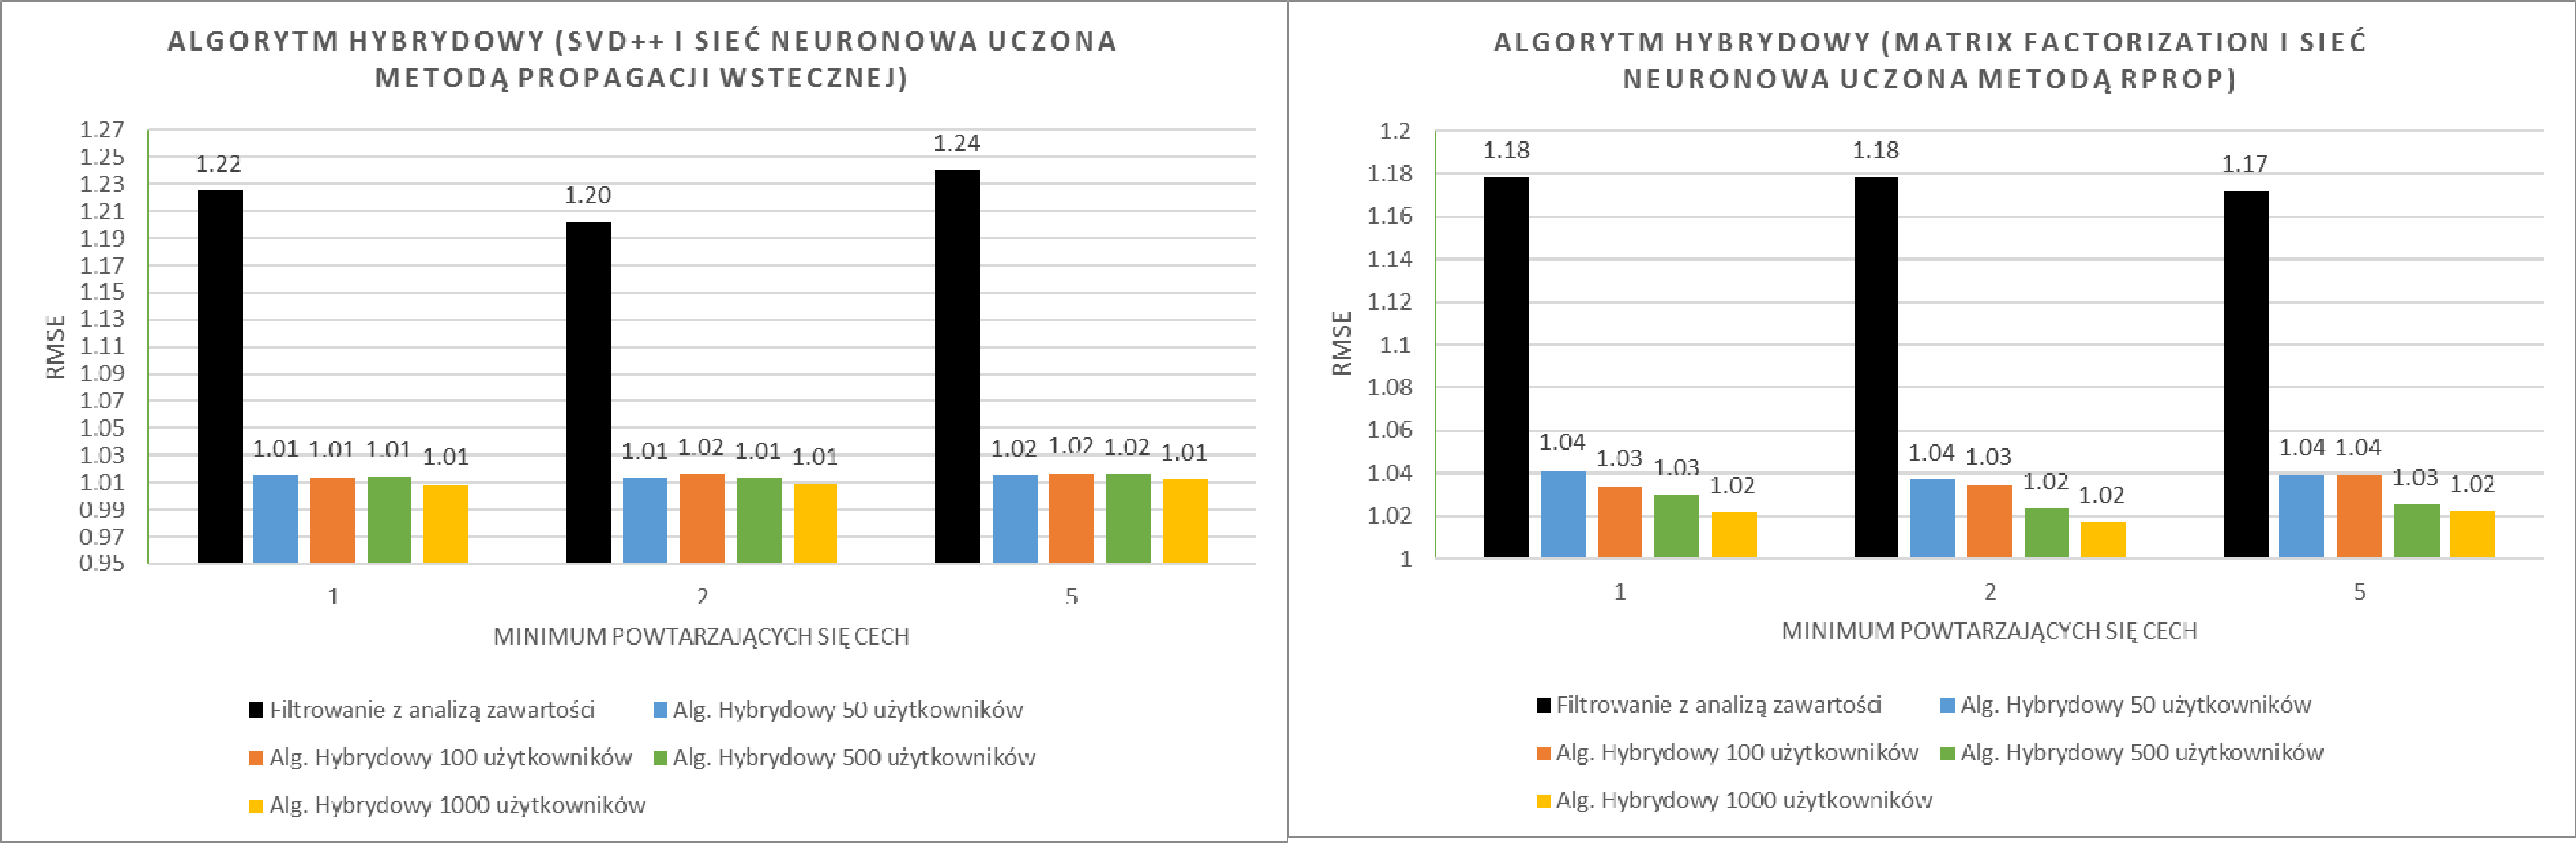
\includegraphics[width=1\textwidth]{am_exphybrid1_2}			
			\caption{\textbf{Po lewej}: wyniki eksperymentu porównującego działanie algorytmu hybrydowego ,SVD++ i~sieć neuronowa uczona metodą propagacji wstecznej'' z~filtrowaniem z~analizą zawartości z~siecią neuronową uczoną metodą propagacji wstecznej. \textbf{Po prawej}: wyniki eksperymentu porównującego działanie algorytmu hybrydowego ,,matrix factorization i~sieć neuronowa uczona metodą RPROP'' z~filtrowaniem z~analizą zawartości z~siecią neuronową uczoną metodą RPROP (baza AmazonMeta).}
			\label{fig:am_exphybrid1_2}
		\end{figure}
	
		\begin{figure}
			\centering
			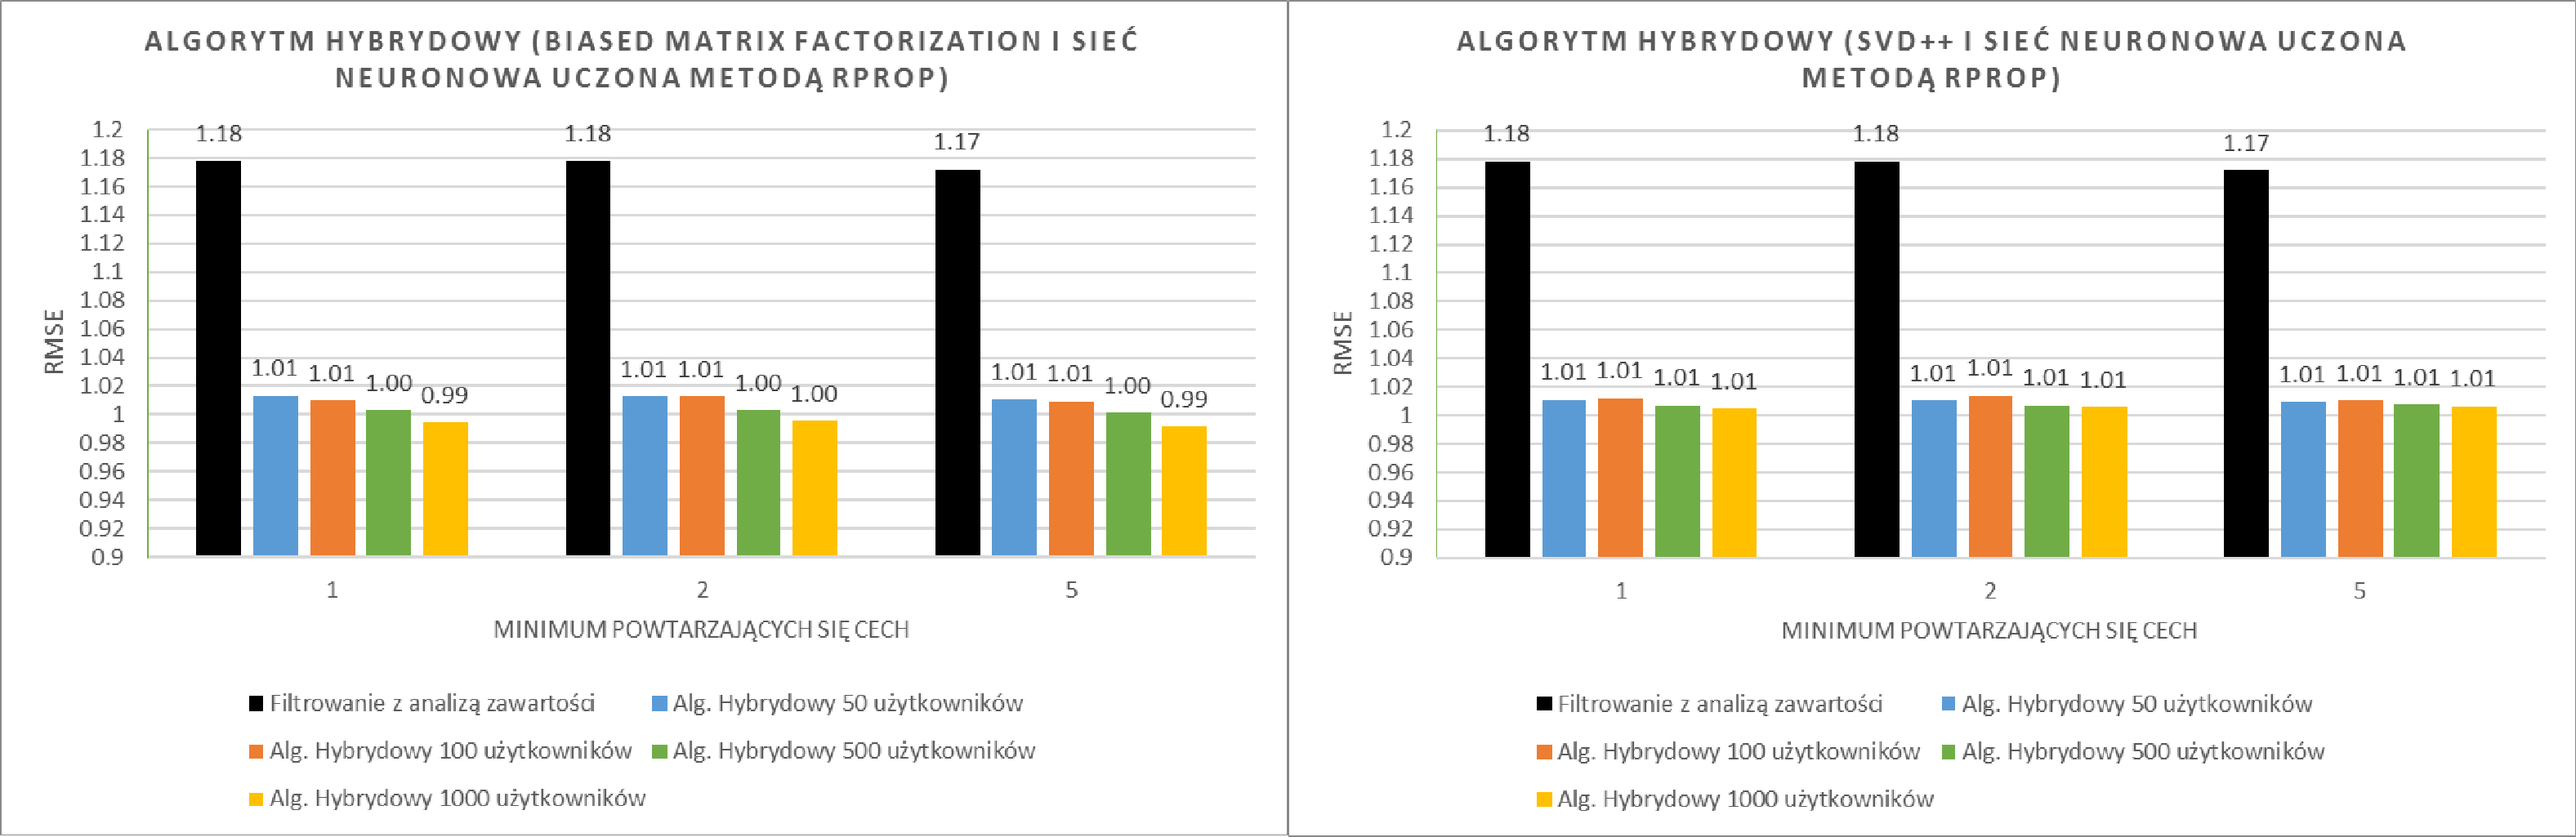
\includegraphics[width=1\textwidth]{am_exphybrid1_3}			
			\caption{\textbf{Po lewej}: wyniki eksperymentu porównującego działanie algorytmu hybrydowego ,,biased matrix factorization i~sieć neuronowa uczona metodą RPROP'' z~filtrowaniem z~analizą zawartości z~siecią neuronową uczoną metodą RPROP. \textbf{Po prawej}: wyniki eksperymentu porównującego działanie algorytmu hybrydowego ,,SVD++ i~sieć neuronowa uczona metodą RPROP'' z~filtrowaniem z~analizą zawartości z~siecią neuronową uczoną metodą RPROP (baza AmazonMeta).}
			\label{fig:am_exphybrid1_3}
		\end{figure}
	
		\begin{figure}
			\centering
			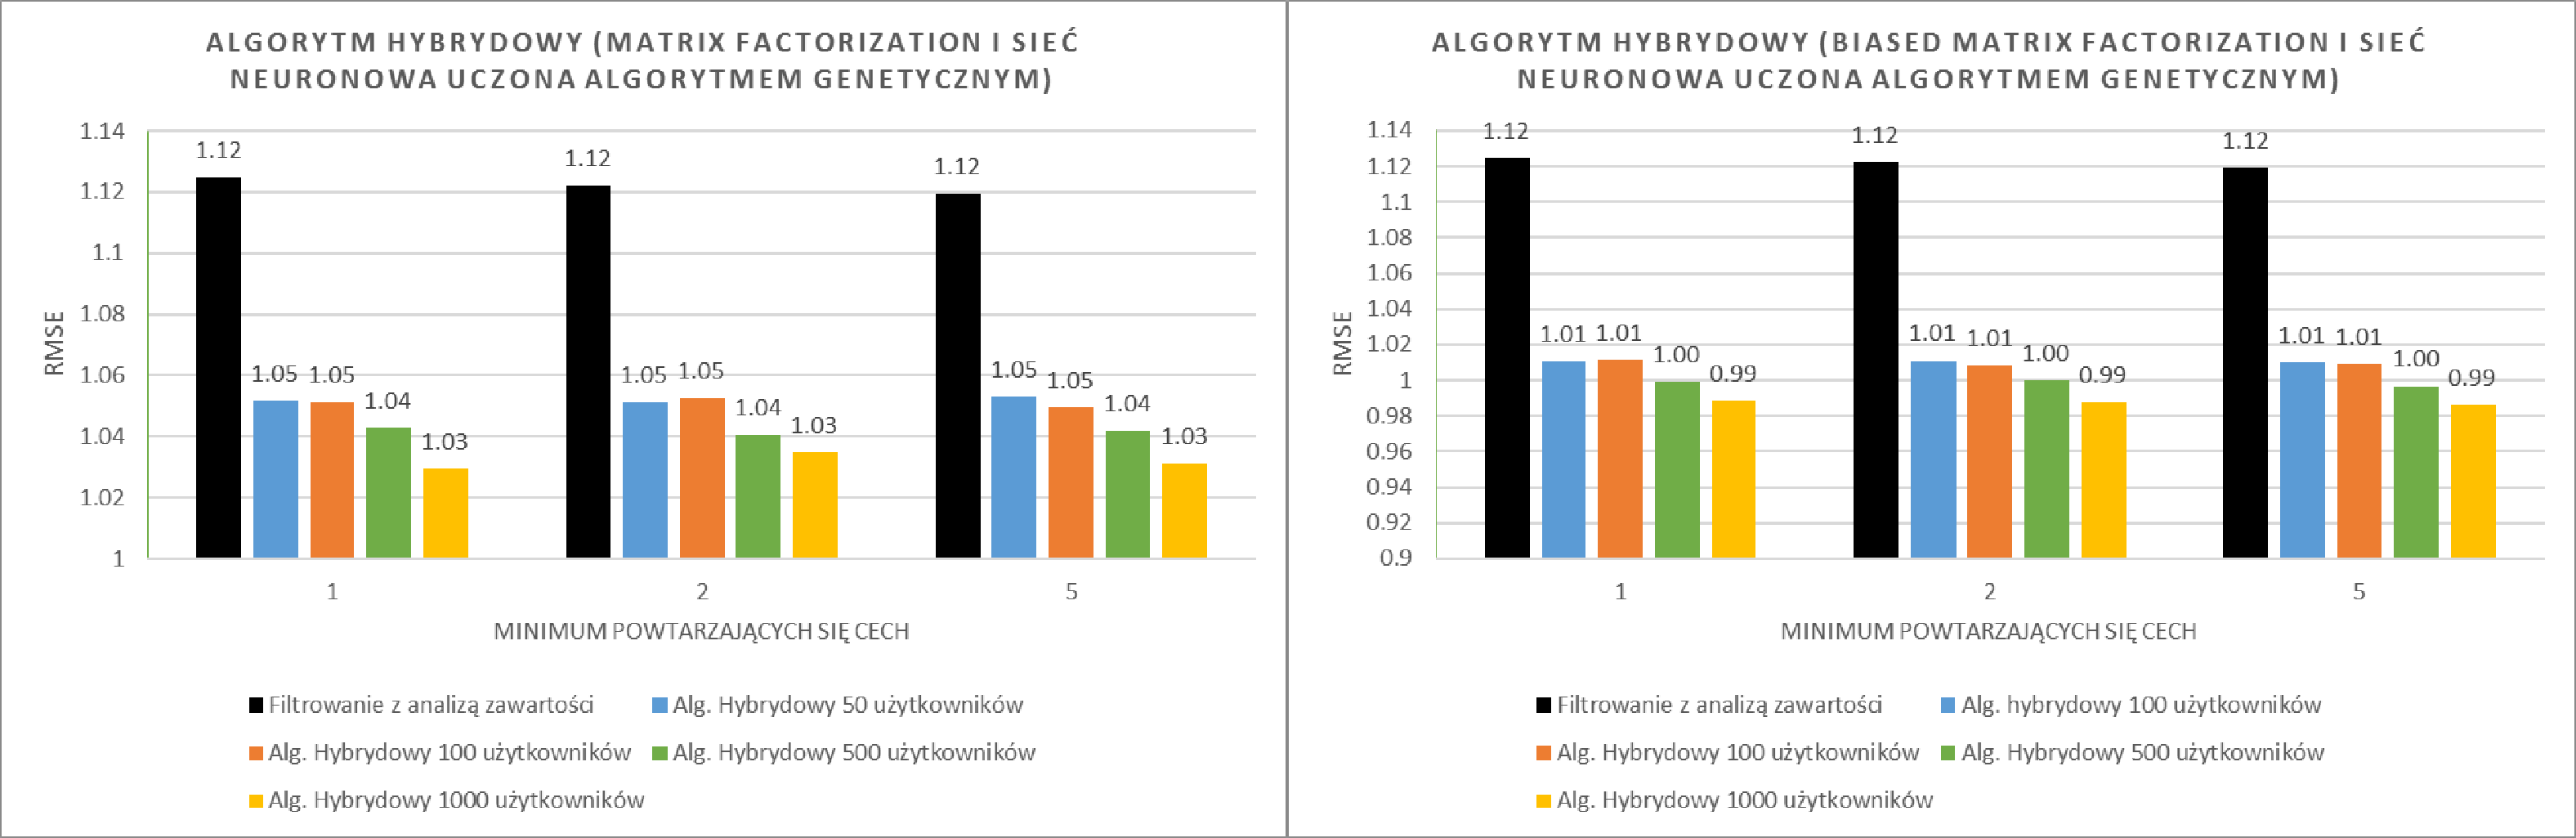
\includegraphics[width=1\textwidth]{am_exphybrid1_4}			
			\caption{\textbf{Po lewej}: wyniki eksperymentu porównującego działanie algorytmu hybrydowego ,,matrix factorization i~sieć neuronowa uczona algorytmem genetycznym'' z~filtrowaniem z~analizą zawartości z~siecią neuronową uczoną algorytmem genetycznym. \textbf{Po prawej}: wyniki eksperymentu porównującego działanie algorytmu hybrydowego ,,biased matrix factorization i~sieć neuronowa uczona algorytmem genetycznym'' z~filtrowaniem z~analizą zawartości z~siecią neuronową uczoną algorytmem genetycznym (baza AmazonMeta).}
			\label{fig:am_exphybrid1_4}
		\end{figure}

		\begin{figure}
			\centering
			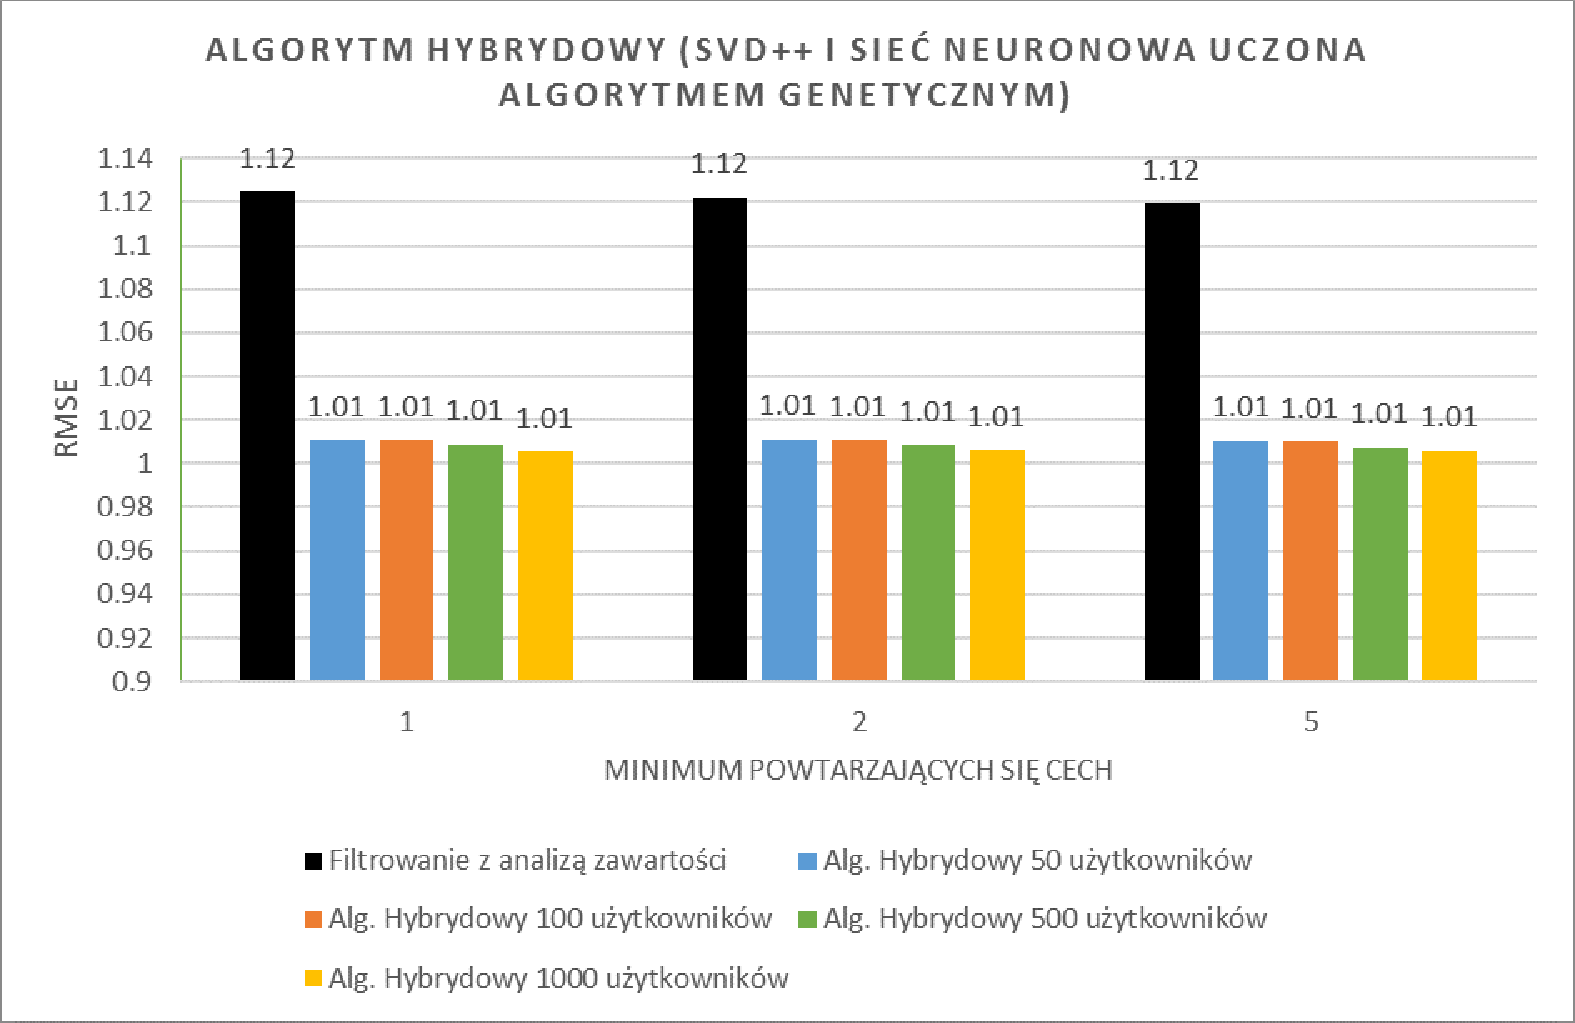
\includegraphics[width=0.5\textwidth]{am_exphybrid1_5}			
			\caption{Wyniki eksperymentu porównującego działanie algorytmu hybrydowego ,,SVD++ i~sieć neuronowa uczona algorytmem genetycznym'' z~filtrowaniem z~analizą zawartości z~siecią neuronową uczoną algorytmem genetycznym (baza AmazonMeta).}
			\label{fig:am_exphybrid1_5}
		\end{figure}

		\subsubsection{Porównanie algorytmów hybrydowych z~filtrowaniem kolaboratywnym}
		
		Wykresy \ref{fig:am_exphybrid2_1} i~\ref{fig:am_exphybrid2_2} przedstawiają porównanie algorytmów hybrydowych z~filtrowaniem kolaboratywnym metodą matrix factorization. Można zaobserwować znaczy spadek RMSE na korzyść algorytmów hybrydowych bez względu ilość powtarzających się cech.
		
		Wykresy \ref{fig:am_exphybrid2_2} i~\ref{fig:am_exphybrid2_3} przedstawiają porównanie algorytmów hybrydowych z~filtrowaniem kolaboratywnym metodą biased matrix factorization. W~większości przypadków algorytmy hybrydowe radzą sobie lepiej. W~przypadku macierzy element-użytkownik liczącej 1000 użytkowników nieznacznie korzystniej wypada algorytm filtrowania kolaboratywnego.
		
		Wykresy \ref{fig:am_exphybrid2_4} i~\ref{fig:am_exphybrid2_5} przedstawiają porównanie algorytmów hybrydowych z~filtrowaniem kolaboratywnym metodą SVD++. Tutaj również widać przewagę algorytmów hybrydowych.
		
		\begin{figure}
			\centering
			\includegraphics[width=1\textwidth]{am_exphybrid2_1}			
			\caption{\textbf{Po lewej}: wyniki eksperymentu porównującego działanie algorytmu hybrydowego ,,matrix factorization i~sieć neuronowa uczona metodą propagacji wstecznej'' z~filtrowaniem kolaboratywnym metodą ,,matrix factorization''. \textbf{Po prawej}: wyniki eksperymentu porównującego działanie algorytmu hybrydowego ,,matrix factorization i~sieć neuronowa uczona metodą RPROP'' z~filtrowaniem kolaboratywnym metodą ,,matrix factorization'' (baza AmazonMeta).}
			\label{fig:am_exphybrid2_1}
		\end{figure}
		
		\begin{figure}
			\centering
			\includegraphics[width=1\textwidth]{am_exphybrid2_2}			
			\caption{\textbf{Po lewej}: wyniki eksperymentu porównującego działanie algorytmu hybrydowego ,,matrix factorization i~sieć neuronowa uczona algorytmem genetycznym'' z~filtrowaniem kolaboratywnym metodą ,,matrix factorization''. \textbf{Po prawej}: wyniki eksperymentu porównującego działanie algorytmu hybrydowego ,,biased matrix factorization i~sieć neuronowa uczona metodą propagacji wstecznej'' z~filtrowaniem kolaboratywnym metodą ,,biased matrix factorization'' (baza AmazonMeta).}
			\label{fig:am_exphybrid2_2}
		\end{figure}
		
		\begin{figure}
			\centering
			\includegraphics[width=1\textwidth]{am_exphybrid2_3}			
			\caption{\textbf{Po lewej}: wyniki eksperymentu porównującego działanie algorytmu hybrydowego ,,biased matrix factorization i~sieć neuronowa uczona metodą RPROP'' z~filtrowaniem kolaboratywnym metodą ,,biased matrix factorization''. \textbf{Po prawej}: wyniki eksperymentu porównującego działanie algorytmu hybrydowego ,,biased matrix factorization i~sieć neuronowa uczona algorytmem genetycznym'' z~filtrowaniem kolaboratywnym metodą ,,biased matrix factorization''(baza AmazonMeta).}
			\label{fig:am_exphybrid2_3}
		\end{figure}
		
		\begin{figure}
			\centering
			\includegraphics[width=1\textwidth]{am_exphybrid2_4}			
			\caption{\textbf{Po lewej}: wyniki eksperymentu porównującego działanie algorytmu hybrydowego ,,SVD++ i~sieć neuronowa uczona metodą propagacji wstecznej'' z~filtrowaniem kolaboratywnym metodą ,,SVD++''. \textbf{Po prawej}: wyniki eksperymentu porównującego działanie algorytmu hybrydowego ,,SVD++ i~sieć neuronowa uczona metodą RPROP'' z~filtrowaniem kolaboratywnym metodą ,,SVD++'' (baza AmazonMeta).}
			\label{fig:am_exphybrid2_4}
		\end{figure}
		
		\begin{figure}
			\centering
			\includegraphics[width=0.5\textwidth]{am_exphybrid2_5}			
			\caption{Wyniki eksperymentu porównującego działanie algorytmu hybrydowego ,,SVD++ i~sieć neuronowa uczona algorytmem genetycznym'' z~filtrowaniem kolaboratywnym metodą ,,SVD++'' (baza MovieLens).}
			\label{fig:am_exphybrid2_5}
		\end{figure}
		
		\subsubsection{Porównanie uśrednionych wartości}
		
		Podobnie jak dla bazy MovieLens aby porównać efektywność poszczególnych algorytmów otrzymane wyniki zostały uśrednione. Rezultat przedstawia wykres \ref{fig:am_exphybrid}. Najlepsze rezultaty otrzymane zostały również dzięki algorytmowi hybrydowemu "biased matrix factorization i~sieć neuronowa uczona algorytmem genetycznym". W~porównaniu do rezultatu osiągniętego za pomocą filtrowania z~analizą zawartości (propagacja wsteczna) RMSE zmalało o~ $18,07\%$. W~porównaniu do najefektywniejszego algorytmu nie-hybrydowego, algorytmu filtrowania kolaboratywnego (SVD++) RMSE zmalało o~$4,07\%$.
		
		\begin{figure}
			\centering
			\includegraphics[width=1\textwidth]{am_exphybrid}	
			\caption{Wykres przedstawia porównanie wyników działania algorytmów hybrydowych (słupki niebieskie) z~algorytmami filtrowania kolaboratywnego (słupki czarne) i~filtrowania z~analizą zawartości (słupki szare) (baza AmazonMeta).}
			\label{fig:am_exphybrid}
		\end{figure}
		
		\subsection{Podsumowanie}
		
		Poszczególne algorytmy osiągnęły różne wyniki na testowanych bazach danych. Wynika to z~różnej konstrukcji tych baz: innego zagęszczenia danych w~macierzach użytkownik-element, innej liczbie atrybutów elementów oraz innej częstotliwości powtarzania się danych atrybutów. Mimo tego w~każdym przypadku większość algorytmów hybrydowych zawsze wypadło lepiej niż samo filtrowanie kolaboratywne i~samo filtrowanie z~analizą zawartości. 
	

\chapter{Wnioski}
\shortTitle{Wnioski}

	Celem niniejszej pracy było opracowanie i~zbudowanie hybrydowego algorytmu rekomendacji wykorzystującego metodę filtrowania kolaboratywnego i~uwzględniającego model elementu rekomendowanego. Przedstawiony algorytm łączy ze sobą metody filtrowania kolaboratywnego i~filtrowania z~analizą zawartości. Ponadto, proponowany system jest uniwersalny. Algorytm osiąga lepsze wyniki niż algorytmy składowe, niezależnie od podpiętego zbioru danych pod warunkiem, że ten zawiera oceny elementów i~ich charakterystykę wyrażoną zbiorem cech.

	Mechanizmy rekomendacji wykorzystywane są przez dostawców wielu usług internetowych takich jak YouTube, LastFM, Pandora, Netflix, Filmweb, Allegro, Amazon i~wiele innych. Motywacją do podjęcia się tematu był fakt, iż mimo że techniki rekomendacji znane są od wielu lat i~są szeroko stosowane, to wciąż są niedoskonałe. Ponadto większość prac tego typu testuje nowe proponowane rozwiązania tylko na jednej bazie danych. Niniejsza praca proponuje rozwiązanie, które działa niezależnie od domeny z~której pochodzą dane.
	
	Do podstawowych technik należą: filtrowanie z~analizą zawartości, filtrowanie kolaboratywne, filtrowanie demograficzne, filtrowanie z~analizą domeny wiedzy, filtrowanie z~analizą społecznościową i~systemy hybrydowe. 
	
	W niniejszej pracy zaproponowana została implementacja filtrowania z~analizą zawartości wykorzystująca sieć neuronową uczoną (zależnie od wariantu) algorytmami propagacji wstecznej, RPROP i~genetycznym. Stworzony został model, który w~sposób uniwersalny odwzorowuje oceniane elementy wraz z~ich cechami. Ponadto, proponowana implementacja oferuje możliwość ustawienia parametrów sieci neuronowej (maks. ilość iteracji nauki, ilość neuronów w~warstwie ukrytej sieci, współczynnik bezwładności, współczynnik uczenia, parametr funkcji aktywacji, rozmiar populacji algorytmu genetycznego) i~parametrów analizowanych danych (minimalna liczba powtarzających się cech).
	
	Do filtrowania kolaboratywnego wykorzystane zostały algorytmy matrix factorization, biased matrix factorization i~SVD++.
	
	Bazując na powyższych metodach zaproponowana została metoda łącząca zalety filtrowania kolaboratywnego i~filtrowania z~analizą zawartości. Powstało 9 algorytmów hybrydowych: 
	
	\begin{enumerate}
		\item Matrix Factorization i~sieć neuronowa uczona metodą propagacji wstecznej
		\item Matrix Factorization i~sieć neuronowa uczona metodą RPROP
		\item Matrix Factorization i~sieć neuronowa uczona algorytmem genetycznym
		\item Biased Matrix Factorization i~sieć neuronowa uczona metodą propagacji wstecznej
		\item Biased Matrix Factorization i~sieć neuronowa uczona metodą RPROP
		\item Biased Matrix Factorization i~sieć neuronowa uczona algorytmem genetycznym
		\item SVD++ i~sieć neuronowa uczona metodą propagacji wstecznej
		\item SVD++ i~sieć neuronowa uczona metodą RPROP
		\item SVD++ i~sieć neuronowa uczona algorytmem genetycznym
	\end{enumerate}
	
	Z wykorzystaniem platformy .NET stworzona została platforma umożliwiająca przetestowanie wszystkich omawianych w~pracy algorytmów. Zaproponowany ogólny model pozwala (z~pomocą odpowiedniego adaptera) na podpięcie dowolnej bazy danych zawierającej oceny elementów do zaimplementowanego systemu. Czyni to zaproponowane rozwiązanie uniwersalnym.
	
	Algorytmy hybrydowe zostały przetestowane na dwóch zbiorach danych z~różnych dziedzin: baza MovieLens zawierająca oceny filmów i~baza AmazonMeta zawierająca oceny produktów zakupionych w~sklepie Amazon. 
	
	Dzięki zaproponowanym algorytmom hybrydowym udało się osiągnąć wyniki: dla bazy MovieLens RMSE o~8,82\% mniejsze niż w~przypadku najefektywniejszego algorytmu nie-hybrydowego filtrowania kolaboratywnego biased matrix factorization; dla bazy AmazonMeta RMSE zmalało o~4,07\% w~porównaniu do filtrowania kolaboratywnego SVD++. 
	
	Nie jest możliwe jednoznaczne wskazanie optymalnego algorytmu. W~zależności od budowy bazy danych, zagęszczenia danych, ilości informacji o~elemencie różne algorytmy wypadają lepiej bądź gorzej.  Mimo tego we wszystkich wykonanych testach algorytmy hybrydowe okazały się efektywniejsze.
	
	Reasumując powyższe rozważania można stwierdzić, że cel niniejszej pracy został osiągnięty. Przeprowadzone badania potwierdziły, że opracowany algorytm hybrydowy jest efektywniejszy i~sprawdza się niezależnie od domeny z~jakiej pochodzą dane. 

	

%\clearpage
%\appendix
%\chapter{Appendix 1}


\clearpage
%\pagestyle{plain}
%\listofmyfigure
%\listofmyequations
%\listofmyalgorithm
%\clearpage

%\{apalike}%Used BibTeX style is unsrt

\bibliographystyle{iisthesis}
\bibliography{bibliography}

\end{document}

